% 大话处理器
% 大话处理器.tex

\documentclass[12pt,UTF8]{ctexbook}

% 设置纸张信息。
\usepackage[a4paper,twoside]{geometry}
\geometry{
	left=25mm,
	right=25mm,
	bottom=25.4mm,
	bindingoffset=10mm
}

% 设置字体,并解决显示难检字问题。
\xeCJKsetup{AutoFallBack=true}
\setCJKmainfont{SimSun}[BoldFont=SimHei, ItalicFont=KaiTi, FallBack=SimSun-ExtB]

% 目录 chapter 级别加点(.)。
\usepackage{titletoc}
\titlecontents{chapter}[0pt]{\vspace{3mm}\bf\addvspace{2pt}\filright}{\contentspush{\thecontentslabel\hspace{0.8em}}}{}{\titlerule*[8pt]{.}\contentspage}

% 设置 part 和 chapter 标题格式。
\ctexset{
	chapter/name={第,章},
	chapter/number={\arabic{chapter}}
}

% 图片相关设置。
\usepackage{graphicx}
\graphicspath{{Images/}}

% 设置署名格式。
\newenvironment{shuming}{\hfill\zihao{4}}

% 注脚每页重新编号,避免编号过大。
\usepackage[perpage]{footmisc}

\title{\heiti\zihao{0} 大话处理器——处理器基础知识读本}
\author{万木杨}
\date{}

\begin{document}

\maketitle
\tableofcontents

\frontmatter

\begin{figure}[htbp]
	\centering
	
\includegraphics[width=0.7\linewidth]{cover}
	\caption{}
	\label{fig:1}
\end{figure}

\chapter{序一 寻宝处理器的引人入胜之旅}

当出版社的编辑介绍万木杨的这本书给我时,我对书名《大话处理器》是有一定担心的,其一:处理器和计算机的发展几十年来风起云涌,其间有天才的创新、看似偶然的分叉和囿于商业市场考量的成功与失败,一部技术发展史绝不比波谲云诡的社会史逊色。一部“大话”处理器的书会不会流于一部围绕处理器发展种种轶事的大话技术史?读书时固然会津津乐道,兴趣斐然,然而掩卷沉思后,会不会仍然无法对处理器的体系结构有更清晰的认识?其二:处理器的发展是和软件、操作系统的发展互为作用的,其中很多技术点和概念都值得深入讨论。采用“大话”的方式能否既保证技术书籍叙述的准确性,又不至于陷入对某些概念旁征博引的“Rat hole”式的罗列,而变得像很多剪贴式编著的IT书籍一样?

但其后数次断续读稿时沉浸其中的体验打消了我的顾虑。我几次阅读书稿都是在出差途中(如飞机上),一个很深的体验是一旦开始阅读就不愿终止,一直读到不得不将书稿收起走路为止。另一个体验是,从任何一个间断点,都可以把本书当作入口,去找寻别的书籍进一步深入学习其中的一些关键技术,就好像函数调用一般,这是我所期望的带领读者进入处理器世界的导游书籍,因此非常愿意向广大的读者推荐这本书。

在技术书籍的阅读中,我偏爱爱因斯坦阐释的方法——“在所阅读的书中,找出可以把自己引向深入的东西,把其他的一切统统抛掉。”这就是抛掉使大脑负担过重和把自己诱离要点的一切。

万木杨的这本书,在选材上围绕处理器的核心技术,从计算机发展的形态、历史展开叙述,在简略介绍了处理器的周边设备后,迅速深入处理器的抽象模型,以计算机软件生态系统中最重要的指令集体系结构ISA切入到探索处理器的微架构,对处理器微架构的一些核心技术,如流水线、乱序执行、指令级并行、线程级并行、缓存结构和算法、缓存一致性等概念,言简意赅地做了原理阐释。而了解这些核心概念,是理解其后第六章优化代码效率的基础。窃以为这些章节是本书的“hardcore”,很值得一读。

在本书的写作风格上,作者运用了很多崭新的网络元素和鲜活的比拟来厘清概念,比如用《我的兄弟叫顺溜》中的顺溜装配子弹的例子来开展指令流水线的讨论,既不流于表面、为举例而举例,又一以贯之地将每个案例充分展开、把问题说透,这样的例子在本书中比比皆是,也是我推荐该书的原因之一。这体现了“抛掉使大脑负担过重”的原则,以及作者对所叙述的技术的深度把握。没有这种把握,是很难用好这种比拟的,反而容易变成“画虎不成反类犬”。

由于长期从事性能优化工作,此前也出版了一本针对并行优化指南的书,因此对本书中阐述并行处理和编写高效代码的章节仍觉意犹未尽,这让我想起了两件事:

其一,我在2001年左右从事针对多核DSP的手写汇编代码优化工作,就是本书里所总结的VLIW并行实现机制,当时一个很深的感触是,人类大脑的并行度很低,至少在汇编这个层级,能够持续对多个计算单元实现高效并行处理编程的上限恐怕就是四级并行了,人的大脑有所谓“一心不可二用”的限制,因此,此后在IA平台上,多核、多进程一直到大规模集群的并行开发的方向就很清楚了,就是必须依赖高级语言的开发工具,支持并行实现的编译器、数学库和线程,MPI进程追踪工具和类似Vtune这样的指令微架构行为的示波器,来解放人的大脑。另一方面就是开发新的并行编程模型和语言,进一步释放多核处理器的性能。

其二,在一本论述并行超级计算机体系架构的英文专著上,我曾读到一段话,似可借来总结处理器性能发展的方向。即,要做快、做好一件事,基本上有三种方法。一是把事情本身缩短、少做事,这就是处理器流水线效率、分支预测命中率等等技术的发展,体现在软件上就是更好的算法和更短的代码关键路径。二是做得更快、更勤些,这就是处理器上更多的浮点计算单元、更高效的缓存、新的高效指令集直到AVX这样的高密度向量计算指令。三是让别人去做或者和别人一起做,这就是并行,多线程和多进程的并行工作。处理器的发展,从性能上看,基本上也可以归为上述三点,比照本书的结构,读者也可以做个归纳。

未来的发展,我们看到了SOC的兴起,我们看到CPU和GPU的混合计算,我们也看到英特尔即将推出的、针对大规模并行应用、集成众核架构的协处理模式的处理器。正如丘吉尔所言,“你能看见多久的过去,就能看见多远的未来”。回顾本书中提到的那些引人入胜的处理器技术的来龙去脉,背后的技术原因或是市场竞争要素,奇妙之处在于,处理器的技术史是我们创造出来的,而身处其中之人却难以知晓,那就让我们“把其他的一切统统抛掉”,一起踏上本书寻宝处理器的引人入胜之旅!是为序。

何万青 博士

英特尔数据中心产品部 高性能计算/工作站架构师

\chapter{序二}

发明第一台计算机的科学家们在发明当初应该不会想到,目前计算机的使用就像水银一样无孔不入地渗透到人类社会的各个方面,并且随着电子、光电子、材料、信息、网络技术的不断朝前发展,会进一步对人类产生巨大影响,人类将越来越依赖计算机技术。

目前许多电子产品并没有明显的计算机三个字出现在其产品说明书上,但实际上,几乎所有智能或部分非智能的电子产品都有一个心脏——CPU核(计算处理单元)在那里跳动。这个心脏的计算能力,根据产品的需求,它可以超级强大到一秒钟完成50亿次运算;其大小根据产品需求,也可以小到只有几十个微米以下,同时还具有很强的计算能力,从而使得这个心脏的功耗可以很小。在这个心脏周围配上相关的硬件、软件就成为一个智能的电子产品。

对大多数人来讲,计算机是一个谜一般的东西。但由于是人类发明了计算机,是人类在使用计算机,而且计算机已经成为人类社会不可缺少的重要组成部分,因此使用计算机的人应该或多或少对计算机有所了解。但如何获得这方面的知识呢?随便到书店或网上去搜索,给出的都是专业的解释。由于计算机产品是一个系统,涉及到与计算技术有关的方方面面,因此要全面、完整、很容易地了解系统的知识,对非从事这行的普通人来讲确实很困难。

万木杨让我给他的新书写一个序,我看完《大话处理器》,觉得这本书的主要对象就是为了这些想了解这个谜的读者。万木杨在计算机、通信领域工作多年,在这方面积累了很强的专业知识,而且博学多才,文采出众。在介绍计算机及其相关知识时,他用了很多与人们日常生活相关的事物来进行对比,一步一步地帮助读者深入。

本书不仅仅是对计算机的核心技术——CPU进行了介绍,而且涉及与CPU相关的多个方面,包括硬件、软件等等,对一般从事电子产品设计的专业人士来讲,也是一本非常有用的参考书。相信这本书不仅能给广大读者带来计算机方面的基础知识,而且能帮助大家用好计算机以及越来越多的智能产品。

周峰

原浙江大学信息与电子工程系副主任、博导

原Aitech公司工程部主管

原VIMICRO公司系统工程部资深总监

华为美研所专家

\chapter{序三 处理器——半导体巅峰,纵横四十年}

处理器,这个半导体科技的最前沿,在过去40年的信息化浪潮中充当了发动机的核心角色。它是如此高贵、而又如此普及,各国政府争相投资,普通家庭却人人拥有;它是如此流行、而又如此神秘,不只工程师们在苦苦探索、寻微知著,就连业余的发烧友们也都对它津津乐道、魂牵梦绕。

木杨兄弟是一位热情而又执着的DSP领域工程师,多年的工作,让他在DSP领域驾轻就熟。在他自由翱翔后,不肯专美,利用自己的专业背景和业余时间,试图把复杂、专业的处理器技术通俗化,与大家分享,正所谓“独乐乐不如众乐乐”,真有侠客之风也。

本书的主人翁——处理器,自发明之初至今已有40多年的历史了,相比浩瀚的宇宙,它是何其短暂,却又是如此的丰富多彩,可以说,处理器的发展,印证着人类信息社会飞速发展的轨迹。

第一次作序,诚惶诚恐,只盼能够给读者一个兴趣盎然的开始,其他无须赘言,就此打住,仅以华为公司2010年处理器技术大会闭幕时的一首小诗开始,引导读者进入探寻处理器神秘硅片奥秘之旅。

华为2010年处理器技术大会闭幕词:

处理器生态圈40年,沧桑沿革,英雄如过江之鲫,童叟未必不珠矶,泰斗亦只能为一家之言。然,盛况者唯在于开放互师,集摸象之和,共探未知!

附拙文以记:

沙中求世界,乾坤即微丸;

格物无穷尽,妙理不待言。

今开三尺坛,八仙恣意展;

四十年沧桑,尽赋谈笑间!

蔡绪鹏

华为处理器行业管理协会会长

公司硬件技术开发部部长

\chapter{前言}

正如广告语说的那样:处理器无处不在(Microprocessors are everywhere)。每一个成功的男人背后都有一个成功的女人,每一个成功的电子产品里面至少有一个成功的处理器。不管是我们经常使用的计算机、手机、汽车,还是为我们服务但我们不知道它们在哪儿的基站、服务器、交换机等,莫不如此。我们身处的电子世界,是建立在处理器基础之上的。前科技部部长徐冠华曾经发出这样的感叹:“没有自己的CPU芯片,我们的信息产业大厦就如同建立在沙滩上。”正因如此,龙芯、汉芯等芯的一点点风吹草动,总能牵动大家的心。

服务器的处理器被Intel和IBM把持着,PC机的处理器被Intel和AMD把持着,手机、平板电脑上的处理器则是百家争鸣,不仅有传统的高通、博通、TI、Freescale等公司,三星、苹果、nVidia等公司也加入了战团。另外,新的处理器公司也依靠自己在某一方面的独特技术优势而备受追捧,如擅长多核的Tilera、擅长可配置处理器的Tensilica等。

做处理器很难吗?难,也可说不难。说它难,是因为从头设计一款处理器确实很难,说它不难,是因为现在可以买到一大堆的处理器IP核,如ARM核、MIPS核、PowerPC核、Xtensa核等,网上还有开源的处理器核,用这些处理器IP核再搭配一些外围的东西,就可以设计出一款处理器,交由芯片代工厂生产,就得到了一颗处理器芯片。这个行业是越来越开放,越来越“混乱”,也越来越有意思。

本书内容

本书是一本图文并茂、生动幽默的处理器科普读物,全书行文风趣幽默,用类比来解释晦涩的技术,用图画来代替枯燥的文字。本着科技以人为本的理念,本书除了技术外,还介绍了大量人物和公司的故事,供大家闲读。本书站在一个软件工程师的角度来描述处理器,书中没有花篇幅谈论处理器的外设、接口、中断等内容,而是更多地探讨影响处理器性能的流水线、指令并行、数据并行、线程并行、Cache等内容。

说起处理器,自然不能不提计算机,第1章漫游计算机世界,介绍了计算机的前世今生,以及计算机的五脏六腑、七经八脉。

第2~5章从外到内,介绍了处理器的外表和内心结构,处理器的核心技术尽在于此。了解了这几章,我们就能知道一款处理器擅长做什么事情,不擅长做什么事情。第6章向软件人员介绍了怎样编写高效代码,处理器的客户就是程序员,程序员在处理器上开发程序,对处理器了解得越深,编写出来的代码执行效率就越高。

第7章介绍了一大堆的处理器IP公司,现在的人们攒电脑,以后的人们说不定就能攒处理器了。

第8章走进处理器的内“芯”世界,介绍处理器芯片是怎么设计与制造出来的。

本书特色

图多。常言道,文不如表,表不如图,图一来可以节省笔墨,二来可以迅速向读者强化作者的意思,其实汉语本身就是象形字,最早也是从图演化而来,以图代文也是理所当然。

语言生动、幽默,多用类比。一个东西,这样说不容易懂,换一种说法就容易懂了,很多技术也来源于生活,技术和生活实例联系在一起,也更能帮助读者理解、记忆。

知识面广、新颖。本书介绍了大量的公司、人物和故事,也介绍了计算机、处理器、软件、芯片设计与制造。

读者对象

本书的读者对象是对计算机、处理器感兴趣的人员,做软件开发的人员,以及IT、通信、电子、半导体行业的从业人员和大专院校的学生。喜欢技术的看技术,不喜欢技术的看故事。

致谢

感谢漂亮、可爱的曹阳妹妹为本书作画,画工精湛,创意一流。感谢英特尔高性能计算/工作站架构师何万青博士在百忙之中读完本书,并熬夜作序,导致第二天发高烧,在此致上歉意。感谢华为处理器行业管理协会会长、硬件技术开发部部长蔡绪鹏总结了处理器四十年的发展历程,为本书作序(注:根据出版需要,有删减,原文参见作者博客)。感谢原浙江大学信息与电子工程系副主任、博导,华为美国研究所专家,资深硅谷人士周峰博士,在本书的写作与出版上,提出了诸多指导意见,并作序。感谢清华大学出版社王峰松老师为本书的写作与出版殚精竭虑,出谋划策。感谢为我的成长给予过帮助的所有人。

本书包含大量的图片,除了原创的漫画、示意图外,还包含不少历史名人照片、剧照、相关产品照片、互联网娱乐照片等,此外,本书还有少量图片直接引用或者参考了现有的学术示意图,这些图片来源于各大公司官方网站(如Intel、TI、IBM等)、国外著名大学、维基百科等网站,特对这些图片的作者和所有者表示感谢。

本书从2009年7月开始写作,大约花了两年时间,期间做过3次大的结构调整,终于形成了现在的结构。本书接近写成之际,作者在通信人家园论坛里连载了一部分,得到了不少好评,也迅速被置顶、加精、进入论坛首页。该帖在华为公司内部也被多次转载、邮件传播,不少同事的相关培训PPT直接引用作者在书中所绘制的原图,相信本书不会让读者失望。

本书邀请了不少业内专家进行审查,不过也不一定能确保完全准确无误,读者可以访问作者的博客(http://blog.csdn.net/muxiqingyang)或微博(http://weibo.com/muxiqingyang)对本书进行批评、建议、讨论,还可以下载作者为本书所设计的PPT,也可以通过电子邮件(muxiqingyang@qq.com)和作者交流。

万木杨

\mainmatter

\chapter{漫游计算机世界}

从起源中理解事物,就是从本质理解事物。

——杜勒鲁奇

你对以往知道的愈多,对未来就看得愈远。

——温斯顿·丘吉尔

导读——人机大战

1997年5月3日至11日,蝉联12年国际象棋世界冠军的卡斯帕罗夫与IBM公司研制的巨型计算机深蓝进行了一场6局的人机大战,卡斯帕罗夫以2.5分比3.5分的总成绩败给了深蓝。

\begin{figure}[htbp]
	\centering
	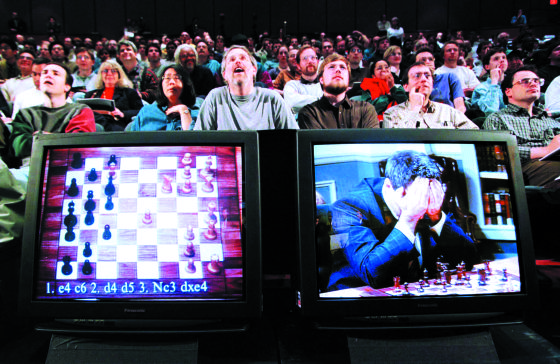
\includegraphics[width=0.7\linewidth]{1}
	\caption{深蓝PK卡斯帕罗夫}
	\label{fig:1}
\end{figure}

2011年2月14日,IBM的计算机Watson继续挑战人类,这次的挑战项目是知识竞赛,它的对手是知识竞赛电视节目“Jeopardy!”有史以来最强的选手Ken Jennings和Brad Rutter,这3个“人”抢答主持人提出的各种稀奇古怪的问题,问题涉及历史、时事、科学、艺术、体育、地理、流行文化、文学与语言、文字游戏等,结果Watson以大比分遥遥领先。

\begin{figure}[htbp]
	\centering
	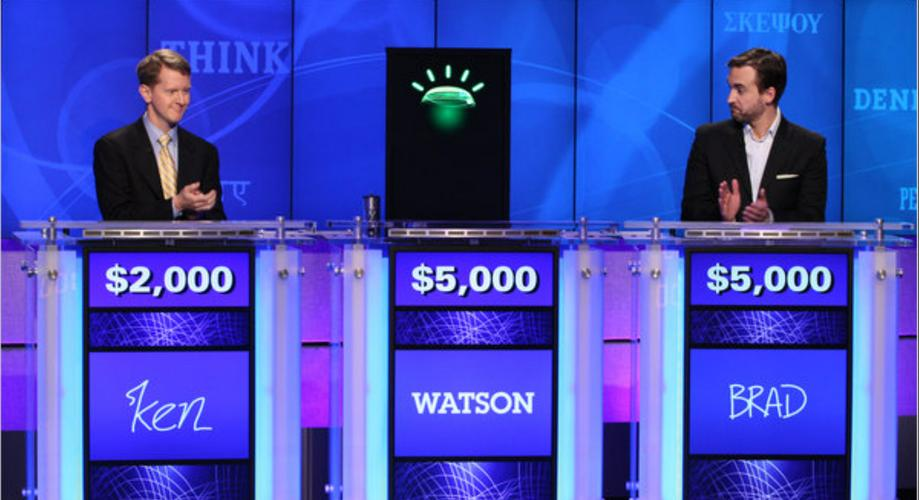
\includegraphics[width=0.7\linewidth]{2}
	\caption{Watson挑战人类}
	\label{fig:1}
\end{figure}

不是人脑不聪明,只是电脑太疯狂。下面我们先来回顾计算机的故事。

\section{计算机的前世、今生、来世}

从起源中理解事物,就是从本质理解事物。

——杜勒鲁奇

你对以往知道的愈多,对未来就看得愈远。

——温斯顿·丘吉尔

地球的任何一部分历史,犹如一个士兵的生活,由长期的无聊和短期的恐怖组成。

——德雷克·V·埃基尔

佛家喜欢谈三世,即前世、今生和来世。今生过得不好,那是因为前世造孽了,不过你也用不着气馁,如果今生好好修行,来世还是可以过好日子的。杜勒鲁奇说,从起源中理解事物,就是从本质理解事物。我们也沾沾佛祖的光,来谈谈计算机的三世。

\subsection{计算机的诞生}

1.计算机之父

=====================================================计算机的家世很混乱,因为有3个人都被人们称为“计算机之父”。他们分别是:查尔斯·巴贝奇(1791—1871,英国人),约翰·冯·诺依曼(1903—1957,匈牙利人,美籍),阿兰·图灵(1912—1954,英国人)。其中冯·诺依曼作为“计算机之父”的知名度最高。

与其浪费时间争论谁做的贡献多一点,不如了解他们都做了哪些贡献。央视《对话》栏目在一期节目中邀请了《功夫熊猫》的导演,当主持人称呼他为“功夫熊猫之父”时,他谦逊地说,我更像是功夫熊猫的叔叔,很多的人一起完成了这项杰作。

计算机不是一个科学发现,而是一个科学和工程结合的系统工程,是无数人共同努力的成果,因此,我们将那些做出突出贡献的人尊称为“计算机之叔”或“计算机之婶”可能更为合适。

2.从计算器到计算机——一字之差,天壤之别

计算机的主要工作就是计算,不管是看视频还是上网,都离不开计算。历史上和计算机最接近的东西,当属计算器。

1642年,法国大科学家帕斯卡发明了加法器,我们在高中学过他的帕斯卡定律。1673年,德国大科学家莱布尼兹发明了乘法器,后来经不断改进,能进行加、减、乘、除、开方全套运算,我们在大学学微积分时听过他的名号。

计算机相比计算器,最大的不同在于它的程序思想。

看帕斯卡笑话,回顾高中物理

一群伟大的科学家死后在天堂里捉迷藏。轮到爱因斯坦抓人,他数到100睁开眼睛,看到所有人都藏起来了,只有牛顿还站在那里。爱因斯坦走过去说:“牛顿,我抓到你了。”牛顿:“不,你没抓到牛顿。”爱因斯坦:“你不是牛顿你是谁?”牛顿说:“你看我脚下是什么?”爱因斯坦低下头看到牛顿站在一块长宽都一米的正方形的地板上,不解。牛顿:“我脚下这是一平方米的方块,我站在上面就是牛顿/平方米,所以你抓到的不是牛顿,你抓住的是帕斯卡。”——引自网络
3.程序思想的来源

1801年,法国人约瑟夫·玛利·亚卡尔创造性地制造了一台织布机。这本来和计算机没有什么关系,不过这台织布机十分的巧妙,它织出来的花样可以通过一串卡片上的孔来决定,人们事先在卡片上打孔来设计织物的花样,机器就可以织出这种花样,颇有点通过软件来控制计算机的概念。这个发明对后世的计算机影响重大,打孔机控制技术就被应用到早期电子计算机的输入设备上。也有人说,计算机是织布机的后代。从这里我们可以看出,创新并不是指完全发明新的东西,把一个领域中的东西搬到另一个领域,也是一种非常好的创新。

约瑟夫·玛利·亚卡尔
4.计算机第一人

真正开始研究计算机和去实现计算机,当从英国人查尔斯·巴贝奇开始。巴贝奇在他的自传《一个哲学家的生命历程》里,写到了大约发生在1812年的一件事:

“有一天晚上,我坐在剑桥大学的分析学会办公室里,神志恍惚地低头看着面前打开的一张对数表。一位会员走进屋来,瞧见我的样子,忙喊道:‘喂!你梦见什么啦?’我指着对数表回答说:‘我正在考虑这些表也许能用机器来计算!’”

巴贝奇的第一个目标是制作一台“差分机”,那年他刚满20岁。10年后,1822年,差分机初战告捷,运算精度达到了6位小数。巴贝奇进一步酝酿运算精度为20位的差分机,然而,当时的机械加工工艺远无法支撑这么高的精度,因此该项目以失败告终。

差分机失败后,巴贝奇提出了一项新的更大胆的设计。他最后冲刺的目标,不是仅仅能够制表的差分机,而是一种通用的数学计算机。巴贝奇把这种新的设计叫做“分析机”。他从法国人约瑟夫·玛利·亚卡尔发明的提花织布机上获得了灵感,分析机设计闪烁出了程序控制的灵光——它能够按照设计者的旨意,自动处理不同函数的计算过程。

后人仿制的分析机

巴贝奇首先为分析机构思了“存贮库”和“运算室”。此外,巴贝奇也构思了送入和取出数据的机构,以及在“存储库”和“运算室”之间运输数据的部件。一个多世纪过去后,现代计算机的结构几乎就是巴贝奇分析机的翻版,只不过它的主要部件由机械变成了集成电路。因此,现代人给巴贝奇封了一个“计算机之父”的称号。

巴贝奇的另一个重要的贡献是在计算机控制中加入了分支控制,使得计算机和计算器分道扬镳。条件控制非常重要,软件工程师都非常熟悉,程序的流程有3类:顺序、分支、循环,分支控制使得计算机可以做很多事,而不像计算器只能做一件事。

巴贝奇不是一个人在战斗,他在研制计算机的过程中,找到了一个志同道合的女助手,她就是英国著名浪漫派诗人拜伦的女儿——爱达·拜伦(也叫爱达·拉弗雷斯,同丈夫姓)。

查尔斯·巴贝奇

爱达·拜伦
5.第一位程序员——居然是个女人

爱达出生不久后父母离异,爱达由母亲抚养成人。深受数学家母亲的影响,她从小就酷爱数学,一直醉心于数学研究。在当时,巴贝奇的机器被认为是没有价值的,是个只会烧钱的废物,巴贝奇拉不到经费,也得不到人们的理解,不过爱达却非常清楚这项工作的意义。爱达负责为这台还没有建成的机器写程序,她创造了子程序、循环的概念。后来美国国防部开发了一种面向对象的高级编程语言,为了纪念这位计算机软件的开山之祖,美国国防部将这种语言命名为ADA(爱达)。ADA语言至今还在计算机的某些领域发挥着重要作用,而爱达也被人们尊称为世界上第一个程序员。

程序员这个职业一般被认为是男性职业,就像我所在的公司,写软件的男女比例都快到10:1了,不想第一位程序员却是个女人,而且是个诗人的女儿,历史真是把玩笑开大了。

巴贝奇和爱达的想法超前世界太多年,当时人们对电还没有太深刻的认识,机械水平也不能支撑分析机的实现,他们终其一生也没法制造出自己所设想的机器。

直到大半个世纪之后,在哈佛大学攻读博士学位的美国青年霍德华·艾肯(H·Aiken),从图书馆积满灰尘的书刊里发现了分析机论文。巴贝奇仿佛还在同他娓娓交谈,为他讲解那台机器的结构,目光中充满着期待的神色。以艾肯所处时代的科技水平,已经能够实现巴贝奇的夙愿。为此,他写了一篇《自动计算机的设想》的建议书,提出要用机电方式,而不是用纯机械方法来构造新的“分析机”。

1944年,在IBM公司提供的100万美元资助下,艾肯研制出著名的Mark I机电式计算机,设计思想几乎就是巴贝奇分析机的翻版,Mark I当时就被用来计算原子核裂变过程。1946年,艾肯发表文章写道:“这台机器能自动实现人们预先选定的系列运算,甚至可以求解微分方程。”这是对巴贝奇预言最好的验证。事隔多年后,已经担任大学教授的艾肯博士谈起巴贝奇其人其事,仍然惊叹不已,他感慨地说:“假如巴贝奇晚生75年,我就会失业。”

巴贝奇和爱达是不幸的,他们生前所作的工作得不到认可,他们将种子种在了地下,辛勤耕耘,但收获的却不是他们。在巴贝奇近80年的奋斗生涯里,屡战屡败,屡败屡战,他始终不放弃自己对崇高理想的追求。正如他经常所说的那样:“不管今天怎样被认为是无用的知识,到后世将会变成大众的知识,这就是知识的生命力。”

巴贝奇和爱达过得很悲催,不过悲催的不仅是他们,还包括下面这位。
6.图灵机

计算机领域一直缺少一个奖项。诺贝尔奖一般只授予基础研究的人,像计算机这样偏向于应用的领域却是很难获奖。1966年,美国计算机协会(Association for Computer Machinery,ACM)设立图灵奖,专门奖励那些对计算机科学研究与推动计算机技术发展有卓越贡献的杰出科学家,图灵为什么能担当大任,因为他是用理论证明计算机可行的第一人。

阿兰·图灵于1912年6月23日出生于英国伦敦。图灵很小的时候就显示出了自己的科学家天分,3岁时,他把玩具木头人的胳膊掰下来种植到花园里,想让它们能长出更多的木头。8岁时,图灵写了一部“科学著作”:《关于一种显微镜》,除了错了几个单词外,还算是有板有眼。

阿兰·图灵

1936年,24岁的图灵发表了一篇论文《On computable numbers,with an application to the entscheidungs problem》(论可计算数及其在判定问题中的应用)。这篇论文被誉为是阐明计算机原理的开山之作。

图灵的著名论文

图灵在这篇论文中,详细描述了一项计算任务是怎么用一种计算机器(Computing Machine)来完成的。下图为图灵机的基本组成:

图灵机基本组成

图灵将人在纸上的计算过程看成是由一系列机械的行为所组成的,数据存放在纸袋上,一次只移动一格,将一系列大的步骤拆成小的步骤,如78×45,先计算78×4,再计算78×5,而78×4又可以再分成7×4和8×4,所有的计算过程最终都将转换成非常小的、机械的操作过程,当前时刻具体执行到哪里通过读写头指示器决定。如果将这种思想和现在的计算机类比一下,就知道:纸袋就像一个存储器,读写头就像是程序指针。现代计算机的思想实际上和图灵机是一样的,图灵后来也参与了计算机的研制工作。

与冯·诺依曼同时代的富兰克尔(Frankel,冯·诺依曼同事)在回忆中说:冯·诺依曼没有说过“存储程序”型计算机的概念是他的发明,却不止一次地说过,图灵是现代计算机设计思想的创始人。冯·诺依曼的作用是使世界认识了由图灵引入的计算机基本概念。

《时代》杂志在评价冯·诺依曼时说:

事实上,从耗资1000万美元的超级计算机到今天的无线电话和菲比玩具上所使用的微小芯片,所有的计算机都有一个共同点:它们都是“冯·诺依曼机”,都是冯·诺依曼基于图灵在20世纪40年代的工作所提出的计算机的基本结构的变种。
图灵的八卦

图灵是一个杰出的密码破译专家,为二战做出重要贡献,比“黄依依”要厉害很多。当时德国采用一种叫做“谜”(Enigma)的加密机,图灵成功的设计出了一种叫做霹雳弹(Bombe)的机器,成功地破译了这台加密机。事实上,生活在那个时代的很多科学家,都或多或少地和战争联系在了一起,如香农也做过类似的工作。

图灵也是人工智能的先驱,他提出了一个模仿游戏试验,后人称为“图灵测试”。该实验把被提问的一个人和一台计算机分别隔离在两间屋子,让提问者对人和计算机进行问答测试。如果提问者分不清回答者是人还是机器,那就证明计算机已具备人的智能。人工智能和计算机的起源其实是一样的,早期的很多科学家研究计算机,主要还是想用它来模拟人类大脑的逻辑思维过程进行运算、推理等。

图灵还是一位运动健将,他在1947年用两小时46分3秒跑完了马拉松,这绝对是个专业级的成绩。

图灵的晚年过得十分凄惨,他是一个同性恋,在当时并不能得到人们的认同,图灵因同性恋而被起诉,职业生涯尽毁。1954年图灵因为食用沾染氰化钾的苹果而死亡。

2009年9月,英国首相布朗因为当年英国政府以同性恋相关罪名起诉图灵并定罪,导致他自杀身亡,正式向图灵道歉。

像图灵这样,活着的时候悲惨,死后被人当成宝的人大有人在,上面说的巴贝奇与艾达也是这样。在三大计算机之父中,就属冯·诺依曼过得最滋润,生前得到的荣誉最高。
7.第一台电子计算机之争

很多课本上都将ENIAC作为世界上第一台电子计算机,并且夸大冯·诺依曼对它的贡献,其实不然。

从1939年~1942年,约翰·阿塔纳索夫(John Vincent Atanasoff)和克利福德·贝利(Clifford Berry)在衣阿华州立大学物理系大楼的地下室建成了世界上最早的电子计算机ABC(Atansoff-Berry Computer),这台计算机就是以他们的名字命名的。

约翰·阿塔纳索夫将设计计算机的思路毫不保留地告诉了毛奇莱(John William Mauchly),1946年,毛奇莱和艾科特(John Presper Eckert)建成了ENIAC计算机,并在世界上首次取得了专利。1973年,美国联邦州立法院判处ENIAC的专利无效,因为它的设计思路源自约翰·阿塔纳索夫的发明,并确认阿塔纳索夫是第一个电子计算机方案的设计者。

阿塔纳索夫

贝利

毛奇莱(左)艾科特(右)

在第二次世界大战期间,美国军队非常迫切地需要对他们设计的新型火炮的弹道进行计算,当时,军方雇佣了成百上千的人力“计算机”,Computer这个词最早是指从事计算的人,到后来才独指计算机。当军方得知电子计算机可以将弹道表的计算时间从几天缩短到几分钟时,军方决定资助ENIAC计划。

1943年,该项目由美国国防部出资,宾西法尼亚大学承建。该计算机直接的目的是在第二次世界大战时为军方计算弹道的轨迹。计划总是赶不上变化,没想到德国1945年就投降了,不过ENIAC的研究没有停止,因为计算机能做的工作远不止计算弹道轨迹这么简单。毛奇莱任首席设计师,艾科特任首席工程师(当时24岁)。建成后,ENIAC是当时世界上最大最强,也是最有影响力的计算机,现在都将它认为是世界上第一台电子计算机。

1997年,为了纪念这台电子计算机诞生50周年,一群宾西法尼亚大学的学生制造了单芯片的ENIAC,这个以前占地1800平方尺、重30吨、耗电170千瓦的庞然大物现在被微缩到只有拇指甲大小的芯片上。
8.冯·诺依曼机

历史上,享有数学家称号的人不少,但是享有大数学家称号的人不多,冯·诺依曼就是其中一个,在他参与ENIAC研制前,就已经是赫赫有名的大数学家了,而且他涉猎极广,会7种语言,他和经济学家摩根一起合著了《博弈论与经济行为》,创立了博弈论。冯·诺依曼有句名言:“如果人们不相信数学很简单,只是因为他们没有认识到生活有多复杂。”

冯·诺依曼于1903年出生于匈牙利的犹太人家族,后来来到美国。1944年,诺伊曼参加原子弹的研制工作,该工作涉及极为困难的计算。1944年夏的一天,正在火车站候车的诺依曼巧遇戈尔斯坦,并同他进行了短暂的交谈。当时,戈尔斯坦是美国弹道实验室的军方负责人,他正参与ENIAC计算机的研制工作。戈尔斯坦告诉了冯·诺依曼有关ENIAC的研制情况。具有远见卓识的冯·诺依曼立即为这一研制计划所吸引,他意识到了这项工作将产生深远的意义。

ENIAC

冯·诺依曼

1944年,冯·诺依曼加入了ENIAC团队,为ENIAC提出了很多好的建议。在冯·诺依曼加入到ENIAC团队中时,ENIAC的研制已经没有什么大的障碍了,人们开始把注意力转向下一代计算机——EDVAC,冯·诺依曼也开始研究新机器的逻辑结构。

1945年6月,冯·诺依曼提交了他著名的101页的“关于EDAC的报告草案”,里面描述了计算机的逻辑结构,尤为重要的一点是提出了“存储程序”的思想。

说来惭愧,我在学校学习计算机的时候,就知道了“存储程序”这4个字,却一直不知道它是什么意思,满以为它是一种非常高深的技术,后来查阅了文献才知道,ENLAC的编程是通过手动设置开关和插拔电缆来实现,“存储程序(stored-program)”的意思就是将程序存储到计算机内部,计算机自动执行。这种思想在现在看来是天经地义的,不过在那时却是个创举。

冯·诺依曼定义EDVAC分为5个部分:①运算单元,②控制单元,③存储单元,④输入单元,⑤输出单元,现在的计算机也都使用这个结构,人们把这个结构的计算机称为“冯·诺依曼机”。
9.逻辑学家和工程师的矛盾

冯·诺依曼的报告一经推出,就掀起了世界的计算机热潮,成为划时代的报告,然而冯·诺依曼在报告中没有署上毛奇莱和艾科特的名字,一个人把风头全占了,这令他们十分的不满,争论的焦点是,EDVAC到底有多少是冯·诺依曼个人的贡献。这个问题可能永远也无法弄清楚。艾科特称他们早就有了“存储程序”的想法,只是还没有实现。

毛奇莱和艾科特还是很有商业头脑的,他们试图将做的工作转换为商品,力争得到ENIAC和EDVAC的专利权,但是由于冯·诺依曼的草案已经散发,EDVAC已经不能申请专利。他们收到了ENIAC的专利,不过后来又被法庭宣布无效。

因为专利的所有权问题,毛奇莱、艾科特和学校发生了分歧,他们于是退出了学校,成立了世界上第一个计算机公司——艾科特—毛奇莱公司。一年后,公司发生亏损,不得不宣告破产,后来被Remington Rand收购,毛奇莱和艾科特于是又专心从事计算机的研究,他们后来又设计出了著名的UNIVAC计算机。

毛奇莱和艾科特离开后,宾西法尼亚大学元气大伤,冯·诺依曼也离开了EDVAC研制小组,回到普林斯顿高等研究院,在那里研制阿艾斯机(IAS)。
10.总结

阿兰·图灵提出了图灵机的理论,证明了研制通用计算机的可能性,约翰·阿塔纳索夫和克利福德·贝利用电子元件制造出了电子计算机的雏形,毛奇莱和艾科特吸收阿塔纳索夫的思想,依托军方的资金支持,制成了第一台通用电子计算机,冯·诺依曼将电子计算机的结构逻辑化、系统化,奠定了电子计算机的系统结构。

\subsection{从军用到民用——飞入寻常百姓家}

\subsection{个人计算机时代——英雄辈出的时代}

\subsection{手机——装在口袋的计算机}

\subsection{无处不在的计算机}

\subsection{计算机的来世}


1.1.2 从军用到民用——飞入寻常百姓家
1.IBM的诞生

IBM对计算机做出了重要贡献,虽然现在更多的涉及信息服务业,但是仍然是计算机领域的重量级选手,服务器、处理器、芯片制造等领域都居于业界前列。

IBM的历史,最早可以追溯到“制表机器公司”。

美国宪法规定,每10年要在全国进行一次人口普查,以便决定每个州议员的人数。最早一次人口普查是1790年,花了9个月时间,到了1880年,由于人口急剧增加,居然花了7年半,这就好比一顿饭吃了4个小时,中午饭还没有消化,又要开始准备吃晚饭了。于是当局认识到:必须要有机器来帮助自动化处理。美国人口普查局拿出一大笔奖金,希望有一个发明者来帮助做这些事情。

所谓重赏之下,必有勇夫,在这个背景下,霍勒里斯应运而生,他发明了机械制表机,并创建了“制表机器公司”。经过多次的转手和重组,最后公司转到了老托马斯·沃森手中,更名为国际商用机器公司(IBM)。

机械制表机

第二次世界战争是机械时代和电子时代的分水岭。IBM自己研制和资助别人研制了几台计算机,而真正帮助IBM在商业上成功的计算机是701计算机。

701计算机研制的动力来自于1950年的朝鲜战争,当时老托马斯询问美国政府:公司能为战争做什么?他马上被告知:给国防部捐一台大型的计算机。

1951年,IBM着手开发这台计算机,同时聘请冯·诺依曼担任公司的科学顾问,1952年IBM完成了701计算机的开发,后来又生产了18台,几台送给了政府,几台卖给了公司,这是世界上最早大规模商用的计算机。

IBM对朝鲜战争的投入,可不只几台计算机。IBM那时以精密机械制造擅长,IBM和另一家公司为美国军方生产M1918A2勃朗宁自动步枪,该枪也是朝鲜战争时期的主力步枪。

20世纪50~70年代,是IBM的黄金年代,IBM在全球计算机行业处于绝对的领导地位,罕有对手。它的企业标志——IBM,每个字由8根蓝条拼成,它的销售人员,一律穿着深蓝色的西服,衬托出IBM不可一世的轮廓,人们开始把IBM称作“蓝色巨人”。
2.小型机的兴起

随着战争的结束,军用计算机的时代已经过去,随之而来的是公司和学校对计算机的需求大增。一大批新的计算机公司应运而生,其中的佼佼者就是数字设备公司(DEC)。

1953年冬天,有一个年轻的工程师在IBM实验室大门外,信誓旦旦地说:“我要在IBM的地盘上将IBM击败”,这个人就是Kenneth Olsen。

1957年,Kenneth Olsen创立了DEC公司,为了不引起IBM的注意,防止它打压,公司的名字和产品的名字起得非常有讲究,DEC是Digital Equipment Company的缩写,故意不涉及计算机字眼。1959年,DEC的第一台计算机PDP-1(Program Data Processor)上市。相对于IBM的庞然大物,PDP-1只有冰箱这么大,可以说是小巧玲珑。Olsen也获得了“小型机之父”的称号。到了70年代,DEC成为与IBM齐名的世界第二大计算机公司,事业到达了巅峰,不过DEC却一直没有能够打败IBM。

Kenneth Olsen——小型机之父

华人与计算机

值得一提的是,计算机的发展史上有两个华人做出了突出贡献。

朱传榘,他参与了ENIAC设计,获得了1981年计算机先驱奖。

王安,他发明了“磁芯存储器”等多项技术,1988年,被选入美国发明家名人堂。王安创办了王安电脑公司,曾经红极一时,不过后来王安执意将公司传给自己的儿子,再加上其他一系列的失误,公司最终倒闭。

朱传榘

王安
1.1.3 个人计算机时代——英雄辈出的时代

什么是历史,什么是英雄,是英雄造就了历史,还是历史成就了英雄?个人计算机时代正是个英雄辈出的时代!这个时代属于Intel,Microsoft,Apple,IBM,HP……。

个人计算机发展历程
1.Intel诞生
硅谷

1955年秋天,“晶体管之父”肖克利从加利福尼亚商人Arnold Beckman那里得到了资金支持,回到了自己的故乡加利福尼亚的Palo Alto创立了“肖克利半导体实验室”。Palo Alto同时也是斯坦福大学和惠普的所在地,这里是一个狭长的山谷,空气清新,气候宜人,当地人叫做Bay Area(湾区)。肖克利把半导体带到了这里,这之后的几十年,这里成为了举世闻名的“硅谷”,据说,加州每年制造的晶体管数目比下的雨滴还多。HP、Intel、Cisco、3Com、Sun、AMD、Oracle、Apple、Adobe、Yahoo、Google、Facebook等公司的总部都建在这里。

Google总部

Facebook总部

山不在高,有仙则名。谷不在深,有硅则灵!

肖克利从全国招了一批有才华的年轻工程师、物理学家、化学家。肖克利是一个优秀的科学家,但却不是一个优秀的管理者。他在贝尔试验室时,总认为别人抢走了本属于自己的荣誉,因此在公司里,所有的构思和发展方向都由他来决定,他所雇佣的那些有才华的人,在他严厉的管理方式下无休止的工作着。1957年,以Robert Noyce和Gordon Moore为首的8个人找到了Beckman,要求解除肖克利的管理职务,只允许肖克利作为一个技术顾问,Beckman认真的考虑了一个月,最后还是决定让肖克利继续领导。随后,后来被称为“硅谷八叛将(Traitorous Eight)”的这8个人离开了公司。
Robert Noyce

“硅谷八叛将”辞职后,他们组建了一个名为Fairchild Semiconductor(仙童半导体)的公司,由Fairchild Camera and Instruments公司提供资金支持。Noyce任总经理。

当时,Noyce和德州仪器的Jack Kilby分别发明了集成电路,2000年,瑞典皇家科学院决定把当年的诺贝尔物理学奖颁给集成电路的发明人,但当时Noyce已亡故,由于诺贝尔奖在传统上不授予已亡故的科学家,因此Kilby独享了此项殊荣。

仙童半导体公司在Noyce的精心运筹下,业务迅速地发展。同时,一整套制造晶体管的平面处理技术也日趋成熟,这得益于“硅谷八叛将”之一的Jean A. Hoerni,他发明了半导体制造工艺中至关重要的平面处理技术,极大地降低了半导体器件的价格,为集成电路的成功创造了前提,从而获得1980年的计算机先驱奖。

后来,仙童半导体的母公司不断把利润转移到东海岸,使得创业团队十分恼火。于是,典型的资方和管理团队的矛盾出现了。8叛将中的7个重新出逃创业,其中,Robert Noyce和Gordon Moore于1968年创立了Intel(INTegrated Electronics的缩写)。AMD、美国国家半导体、LSI Logic、VLSI Technology、Intersil、Altera和Xilinx等业界众多巨擘的创始人都来自仙童半导体。苹果公司的乔布斯有这样的比喻:“仙童半导体公司就像个成熟了的蒲公英,你一吹它,这种创业精神的种子就随风四处飘扬了”。由于“硅谷”很多企业都和Noyce有直接或者间接的关系,Noyce更是被人送了一个绰号——“硅谷市长”。

硅谷八叛将,各个身怀绝技并事业有成
Gordon Moore

Gordon Moore在国内比Noyce更出名,因为大家耳熟能详的摩尔定律就是他说的,关于摩尔定律有多个版本,最常见的版本是集成电路上晶体管的数目每18个月翻一番,也有每一年翻一番和每两年翻一番的版本。摩尔后来自己说:“摩尔定律源自1965年我为《电子学》撰写的文章。我预见到,我们将制造出更复杂的电路从而降低电器的成本——根据我的推算,10年之后,一块集成电路板里包含的电子元件会从当时的60个增加到6万多个。那是个胆大的推断。1975年,我又对它做了修正,把每一年翻一番的目标改为每两年翻一番。”(引自Intel网站)

不管是12个月,还是18个月,还是24个月等,摩尔定律描述了一种指数增长的趋势,指数增长是非常吓人的,稍微碰几下就会得到一个天文数字。如果你用信用卡,欠了银行一块钱不还,20年后,银行可能要让你还几十万,这是因为银行是用复利来计算的,复利就是指数,增长势头吓人。
Andy Grove

Andy Grove是Intel的第3个员工,他在业界享有盛名,一方面是因为他领导Intel时,是Intel的鼎盛时期,1997年美国《时代周刊》授予他“年度风云人物”,1998年美国管理学会赋予他“年度杰出经理”,2001年他获得战略管理协会“终身成就奖”,2004年被沃顿商学院提名为25年来最有影响力的CEO。

还有一个原因是Andy Grove写过一本畅销书《Only the Paranoid Survive》,这本书在中国被翻译为:《只有偏执狂才能生存》,这句话一直像圣经一样激励着无数有梦想的人,事实上,很多人理解的这句话的意思和格鲁夫(Grove)说的并不是同一个意思。英文词和中文词在直接翻译时会存在意义偏差,“偏执狂”这个词通俗意思是指一个人目标执着,近乎固执,撞了南墙也不回头,而医学上的解释则是一个人有妄想症,极度的敏感多疑,思想行为固执死板。在《Only the Paranoid Survive》这本书中,作者开篇着重描述让Intel 6周损失4.75亿美金的奔腾芯片浮点bug事故,后面讲的都是变化,以及改变就能生存,不改变就会灭亡。整本书的主题是要想生存,就必须敏感的感受变化,拥抱变化,并采取行动。或许这句话翻译成“唯有惶者才能生存”可能更好,而这句话正是另一企业家任正非的名言,可见英雄通常所见略同。

Robert Noyce

Gordon Moore

Andy Grove
2.Altair诞生

1974年,MITS公司的创始人Edward Roberts(爱德华·罗伯茨)发明了世界上第一台个人计算机(Personal Computer,PC),命名为Altair(牛郎星)。也有人说第一台个人计算机应该是1973年施乐帕克研究中心的奥托(Alto),其实很难找到严格意义上的第一个吃螃蟹的人,因为大家对螃蟹的定义可能不一样。

Roberts给个人计算机定了这样的概念:这是一个体积小、价钱低、可以摆在家里供个人使用,而不是以往在人们印象中那种只有在实验室才能见到的、昂贵的、需要多人操作的庞然大物。

Altair计算机获得成功后,Roberts的生活也发生了巨大的变化,他每天不得不花大量的时间去应付各种公司和媒体,尽管产品的成功给他带来了可观的收入,但他认为“这样的生活是一种煎熬”,1977年,他毅然将公司出售给了一家叫Pertec的公司,自己则进了医学院,后来成了一名医生。

Altair的成功虽然短暂,而且几乎没有太大的名气,但是它却影响了后来成名的3家公司:Intel(Altair计算机采用的是Intel的8080处理器),微软,苹果。

Edward Roberts和他的Altair
3.微软诞生

Altair上市之后,哈佛大学二年级法律系学生比尔·盖茨和他的同学保罗·艾伦立即意识到个人计算机将有无限前景,于是自告奋勇的为Altair开发软件。经过两个月的通宵达旦,他们成功开发出了在Altair上的BASIC编译器。3个月后,盖茨敏锐地察觉到:计算机的发展太快了,等大学毕业,他可能就失去了一个千载难逢的机会。于是1975年6月,盖茨放弃了这所世界上最好大学的毕业证书,毅然选择了退学创业,和保罗一起开创了微软帝国的神话。

微软初期团队
4.苹果诞生

史蒂夫·乔布斯(Steve Jobs)和史蒂夫·沃兹尼亚克(Steve Wozniak)都是电子技术的爱好者,他们经常参加家酿计算机俱乐部(Homebrew Computer Club)的活动,在这里,他们看到了Altair计算机、8080芯片等新的东西并深受启发。1975年,沃兹用MOS Technology公司的6502芯片制造了一台个人计算机,乔布斯立即意识到这个小巧的业余机器有着巨大的商业前景。1976年,乔布斯说服沃兹和乔布斯的另一位好友罗恩·韦恩一起成立了苹果公司,他们把沃兹设计的第一批产品叫做“苹果Ⅰ”。1977年,“苹果Ⅱ”上市,造成了意想不到的轰动,苹果成为个人计算机领域最成功的计算机公司,乔布斯也被《时代》杂志刊登在封面,成为美国人心中的楷模。

史蒂夫·乔布斯(左)和史蒂夫·沃兹尼亚克(右)
5.IBM-PC出世

到了这个时候,谁都知道个人计算机市场是个巨大的金矿,计算机传统巨头IBM当然也不例外。IBM也曾在个人计算机领域做过尝试,但是并不成功。IBM知道,如果还不能在个人计算机市场有所斩获,自己这个老大哥就要在新时代面前丢人现眼了。

1980年7月,IBM召开高层会议,要对如火如荼的个人计算机浪潮做出反应。唐·埃斯特里奇(Don Estridge)受任于败军之际,奉命于危难之间,担任项目负责人,要在一年之内推出IBM的PC机。

Estridge知道12个月是不可能从头到尾完成开发的,唯一的出路的就是打破传统的什么都做的策略,尽可能的引入已经存在的通用部件。于是,IBM采用了Intel的8088处理器,微软的MS-DOS操作系统,开发出了自己的个人计算机:IBM-PC。IBM的这个决定直接导致了微软和Intel后来的成功。

IBM-PC一经推出,在市场上大受欢迎,随之成为“个人计算机”的代名词。IBM的这种PC机构思设计成为一种“开放式”的体系结构,各个部件模块化发展使得PC机得以迅速发展,正如同社会分工促进社会进步一样,大量的IBM-PC的克隆产品(IBM-PC兼容机)如雨后春笋般的滋生出来,使得PC机价格一泻千里,成为普通群众买得起的产品。

1986年,康柏率先使用Intel的386处理器,迅速抢占了市场,于是IBM从PC行业老大哥的位置上落了下来,一大批新的公司成长起来。
6.图形用户界面出世

20世纪70年代,“苹果Ⅱ”在个人计算机市场引发了一场革命,严重挑战了IBM老大哥的地位;80年代初,“IBM-PC”引发了另一场革命,IBM重新向世界宣告:我才是计算机世界的老大。苹果公司面临空前的生存危机。

为了拯救苹果于危难之中,1983年,乔布斯出奇招,将对计算机一窍不通的美国百事可乐主管销售的约翰·斯卡利请了过来。斯卡利在70年代领导了一场享誉美国的商战,硬是从百年老店可口可乐的虎口中夺食,抢走了半壁份额。斯卡利成名已久,对乔布斯开始并不感冒,不过乔布斯的一句话还是打动了斯卡利:“你是想一辈子卖糖水,还是想改变世界?”

销售技巧是锦上添花,而优质的产品特性才是制胜关键。乔布斯的秘密产品特性就是图形界面。1979年12月,乔布斯和几位苹果的工程师参观了施乐公司(Xerox)的PRC研究中心(Xerox Palo Alto Research Center),他们被PARC的GUI(图形用户界面)深深的吸引了,回来后,他们就把这个想法做到了自己的机器上。1983年,苹果推出Lisa电脑,但是由于成本太高,后来被砍掉。1984年,Macintosh诞生了。伴随着斯卡利狂风暴雨般的宣传攻势,以及Macintosh绚丽的用户界面,苹果又一次打败了自己的老大哥——IBM。和当时的Macintosh比起来,IBM-PC只能用土得掉渣来形容。

Macintosh电脑

为他人做嫁衣裳的施乐PARC

施乐的PARC对计算机领域做出了不可磨灭的贡献,微软、苹果等公司都从它的研究成果中获利不少,不过,施乐自己却获利很少。有两家公司的成立和PARC有直接关系。

PostScript用一种公式描述字母和数字,这样字体在放大、缩小和打印时都能保持同样的清晰度。PostScript技术由两名PARC的研究人员发明,两名发明者后来得到了风险投资,创办了自己的公司,运用这项技术创造出了桌面出版这个全新的行业,这家公司的名字就是Adobe。

在PARC工作的Robert Metcalfe发明了以太网,他随后于1979年创办了著名的3Com公司。
7.微软、Intel双双晋级
微软空手套白狼

IBM在研发IBM-PC时,需要操作系统,比尔·盖茨听到这个消息立即就去找IBM公司,要求合作。IBM本来想使用一个叫做CP/M的操作系统,盖茨祭出免费的绝招,拿下了IBM。盖茨买下了Tim Paterson的QDOS软件,在其帮助下改编成MS-DOS。由于IBM-PC兼容机的兴起,MS-DOS得以大卖,历史上从来没有哪个软件有这么大的用户数,微软依托MS-DOS快速崛起。后来Tim Paterson投奔到微软门下,发现自己设计的操作系统正是微软的金矿,不禁大为恼火,不过此时也已无可奈何。
微软打败苹果

Macintosh的兴起使得GUI深入人心。由于苹果坚持不与IBM-PC机兼容,因此微软决定在IBM-PC上开发出图形用户界面。1985年,微软终于完成了第一版Windows的开发,不过由于不稳定,缺陷多,没有获得成功。直到1990年,Windows 3.0才为微软带来巨大的收益。1995年,Windows 95取得了空前的成功,成为操作系统和个人计算机发展史上的一个重要里程碑。

微软腾飞的这几年,也正是苹果衰落的几年,苹果公司是王小儿过年,一年不如一年。苹果的Mac OS一直死守苹果计算机市场,而苹果计算机在价格、应用程序数量上远不如IBM-PC兼容机,其市场一直在下滑,最终逐渐衰落,只能守住专业市场。其间,斯卡利在董事会的支持下,将乔布斯赶出了由他自己创办的公司,后来又几经换帅,还是无法挽救败局。

期间,苹果也采用了知识产权的方式来抵制微软。苹果将微软告上法庭,指责Windows侵犯自己的操作系统。在法庭上,微软的盖茨指出苹果的窗口式图形界面也是抄施乐的,凭什么你能去施乐拿东西,我就不能从你那顺东西。最后,法庭还是以Windows和苹果的操作系统虽然长得像,但不是一个东西为由,驳回了苹果的要求。

1992年,著名作家罗伯特·克伦格利正式将微软命名为“微软帝国”。借助强大的市场优势和金钱实力,微软就像一个大鲨鱼,运用从任我行那里学到的“吸星大法”,将许多公司创造的技术纳入自己的Windows中,使其成为一个无所不能、无所不包的百宝箱。凡是微软想打击的公司,都逃不出它的魔掌,如Sun公司、网景公司等。一直等到了互联网时代,这种情况才有所好转。

这里八卦一下,微软树敌太多,法律纠纷不断,不过一直没有给公司造成大的影响,这估计和盖茨的法律背景有关系。盖茨在哈佛学的就是法律专业,盖茨的老爸在退休前,是Preston Gates \& Ellis律师事务所的合伙人,这家律师事务所后来更名为K\&L Gates,是全美十大律师事务所之一。
Intel打败Motorola

摩托罗拉是个传奇公司,拥有大公司、著名公司、杰出公司之类称号的公司很多,不过拥有传奇公司称号的公司却很少。

摩托罗拉原名加尔文制造公司,创立于1928年,由创始人之一的保罗·加尔文的名字命名。它最早是生产汽车里的收音机的,摩托罗拉是这种收音机的品牌,由于这个品牌深入人心,因此摩托罗拉干脆将自己公司的名字改成了这个名字。这种现象其实不多,与之类似的还有一家公司,那就是松下,Panasonic是松下在日本国外的品牌,后来松下将公司的名字改成了Panasonic。

摩托罗拉除了在人们熟知的无线通信领域有很强的实力外,在处理器领域也是相当的有竞争力。在前几代处理器中,Motorola同期的产品性能要比Intel的好,Macintosh就是选用Motorola的处理器。不过,由于IBM早期选择了Intel的处理器,后来为了软件的兼容性,IBM-PC兼容机都采用Intel的处理器。随着苹果的衰败,Motorola的通用处理器也相继衰败。苹果后来也开始采用Intel的处理器,Motorola彻底退出了通用处理器市场。由此可见,一开始就站错了队,对后面影响有多大啊。
8.Wintel联盟,一统江湖

随着IBM-PC兼容机的流行,IBM-PC成为行业标准,不过,IBM的PC机却受到了巨大的冲击,IBM在PC上的老大位置后来也被惠普给抢走了。到后来,PC机什么人都可以装,PC行业的利润率也逐年下滑,终于,IBM于2004年底将PC业务卖给了联想。

在整个PC行业,有两家公司的地位是无法替代的,一家是微软;另一家是Intel。计算机的发展已经进入了处理器时代和软件时代,这个时代的主导权落在了对集成电路有着深刻认识的Intel,和对软件有着深刻认识的微软手中。计算机的本质,就在于其可编程,软件的执行需要依赖于操作系统和处理器,Intel处理器上的程序不能在ARM中执行,Windows的程序也不能在Linux下执行,为了使PC上以前的程序能继续运行,就必须使用微软的操作系统和Intel或AMD(只占很少的份额)的处理器。

下面这个图描述了应用程序、操作系统、处理器的依赖关系,应用程序依赖于操作系统和处理器,操作系统依赖于处理器。

程序依赖性

桌面操作系统和桌面处理器是两个相互配合并且极欠竞争的领域,Microsoft和Intel由此获得高额利润,它们同时也是欧美反垄断法的宠儿。

Wintel联盟就是Windows和Intel的联盟,这个联盟在业界还有一个定律,叫做安迪·比尔定律:“What andy gives,bill takes away.”无论安迪给什么,比尔都会把它拿走。

安迪就是Intel的前CEO安迪·格鲁夫,比尔就是微软的比尔·盖茨,作为商业同盟,他们每年会晤两三次(引自格鲁夫的《只有偏执狂才能生存》)。用电脑的人都会有这样的感觉:电脑买来没多久,就会发现慢如蜗牛,又要考虑硬件升级了。现在的CPU越做越快,存储越做越大,但是操作系统、应用软件却是越做越慢,越做越大。说白了,商家喜欢消耗品,不喜欢耐用品。

不过我们也不能完全把矛头指向软件公司,现在软件的功能需求越来越多,为了节约软件开发的时间和成本,编程语言越做越高级,对应着效率也自然越来越低。
9.Wintel联盟真的无坚不摧吗?

Wintel联盟统治PC江湖相当之久,很多处理器公司和软件公司分别向Intel和微软发起了一轮又一轮的攻击,不过都是败多胜少,直到最近几年,情况才有所好转。

比较有名的一家挑战公司是Sun公司,Sun也是一家传奇公司,在鼎盛时期,Sun一家公司的产品包含了整条IT产业链:从处理器,到计算机,到网络,到操作系统,到编程语言,到应用软件一条龙服务,外加股价高得吓人,颇有气吞山河之势。Sun很早就提出了“网络就是计算机”的概念,这也正是现在火热的云计算的思想。Sun挑战Wintel联盟的一大利器就是大名鼎鼎的Java。

Java程序依赖性

Java语言的出现打破了江湖上持续了很长时间的平静,Java应用程序通过Java虚拟机和操作系统、处理器分离开来,使用Java编写的应用程序不再依赖于某个具体的操作系统和处理器,Java程序不只可在x86上运行,也可以在ARM等处理器上运行,只要装一个这一平台上的虚拟机就可以了,这样用户对微软的操作系统和Intel的处理器就没有依赖性了。Java也迅速成为当前的主流编程语言,虽然Java是如此的流行,但是Sun一直没找到通过它盈利的方法。随着x86处理器性能的逐渐提升,Sun赖以生存的工作站逐渐被淘汰,Sun公司一蹶不振,被Oracle买去。

互联网的发展,将各种应用都搬到了网上,浏览器逐渐成为继操作系统之外的又一大用户窗口。Google等公司大力开发基于互联网的服务(软件即服务),来为未来屏蔽操作系统做铺垫。到现在,人们在计算机上使用的大部分功能都能在浏览器上完成。例如,可以在浏览器上写作、看电影、听歌、玩游戏……网景联合创始人马克·安德森(Marc Andreessen)有句名言:在互联网的光芒下,操作系统只不过是一套漏洞重重的设备驱动器。

不管是x86+Windows的PC机,还是ARM+Linux的上网本,又或是ARM+Symbian/Android的手机,都可以使用相同的服务,网络服务对处理器和操作系统的依赖性也越来越小。

网络服务的依赖性

目前手机上最火的操作系统当属Google的Android,Google收购了一个做Linux的团队,从而改造成自己的Android。由于Android使用Java语言进行应用软件开发,因此使得应用软件具有更好的可移植性,处理器不管是x86、ARM、MIPS等,均可以执行Android应用程序,Android操作系统也因此大受处理器厂商和应用软件厂商的欢迎。而处理器领域,最近风头正盛的是ARM,微软的桌面操作系统也提供了对ARM的支持。
1.1.4 手机——装在口袋的计算机
1.分不清的界限

以前人们会问:“你家里有计算机没?”

现在这样问就out了,应该问:“你口袋里有几个计算机呀?”

现在其实已经很难区分手机和计算机有什么区别了,对于很多手机来说,PC机能做的,它能做,PC机不能做的,它也能做,高端手机的性能已经不亚于当年的奔3、赛扬了。

下面这张图描述了各种各样的终端,可能他们之间的区别就在于大小了。

各种各样的终端

桌面计算机:一台体验卓越,为所欲为的电脑

笔记本:一台便于移动,性能较强的电脑

上网本:一台便于移动,价格较低的电脑

手机:一台随身携带,永远在线的电脑
2.大哥大

一身风衣,一队马仔,加上一个大哥大,是20世纪90年代港剧中大哥的经典造型。

大哥大

大哥大是第一代移动通信系统的终端设备,几乎被摩托罗拉公司垄断。
3.手机
诺基亚以小博大

20世纪70年代后,随着数字信号处理技术和半导体技术的发展,基于数字电路和信号处理的第二代移动通信渐渐浮出了水面。为了在第二代移动通信中能够赶超美国,早在1982年,欧洲邮电管理委员会(European Conference of Postal and Telecommunications Administrations)就着手制定新一代的移动通信标准Groupe Special Mobile,简称GSM。第一个投入商业运行的GSM移动通信网络,其局端设备供应商是瑞典的爱立信,终端设备的供应商是芬兰的诺基亚,手机是这个时代的主要通信终端。

在模拟时代,话音质量是手机好坏几乎唯一的标准,摩托罗拉无疑在此方面占有优势。而到了数字时代,不同手机的话音质量相差不像以前那么大,此时手机的功能就变得非常重要了,再到后来手机的外观也变得重要起来。摩托罗拉由于思维的定式,在早期开发数字手机时,仍然以话音质量为核心,功能和外观的设计在同行中常常慢一个节拍。而诺基亚、三星等手机很早就强调手机的功能、使用方便和外观,自然也就超越了摩托罗拉。

手机,一把电子瑞士军刀
iPhone与移动互联网

乔布斯的故事还在继续。

乔布斯是硅谷最传奇的一位。年轻的乔布斯行为偏激,根本是一个不能与之共事的人,他被自己请来的斯卡利在董事会的支持下赶出了苹果。

乔布斯离开苹果后,创立了一家计算机公司NeXT,不过没有翻起大浪。之后,乔布斯买下了好莱坞著名导演、制片人乔治·卢卡斯(导演过《星球大战》)的动画制作组,并将其命名为Pixar(皮克斯)公司,皮克斯公司后来制作了一系列经典的动画片,如《玩具总动员》、《机器人总动员》等,皮克斯上市后,乔布斯赚到的钱比从苹果得到的还多。

这个时候的苹果已经是摇摇欲坠,几任CEO都无力回天,没办法,董事会只得把乔布斯请回来,死马当活马医。被资方赶出公司的创始人不少,但是又被请回来的,就几乎没有了,不过乔布斯还是回来的,因为苹果就像他的孩子一样。

回到苹果的乔布斯历经沧桑,也更成熟。乔布斯的回归重新燃烧了苹果的创新小宇宙。苹果凭借着iPod、iTunes、iPhone、App Store等一系列产品和商业模式创新,又一次站了起来,而且站得更高。

iPhone是手机的经典之作,在iPhone出现之前,从来没有人想过,原来手机还可以这样玩。iPhone之火,不需要多说,就连释道心和尚也使用iPhone。

iPhone模糊了手机和计算机的界限,并引发了移动互联网之热,继苹果的App Store之后,Google、诺基亚、中移动等大的手机厂商、信息服务商也都提供了自己的网上商店。
4.山寨机

某日部门开会,领导在上面吐沫横飞,轻舞飞扬,我们在下面正襟危坐,展现出移情式倾听的样子。突然,一兄弟的手机爆响:“死了都要爱,不淋漓尽致不痛快……”巨大的声响直压领导的麦克风,引来大家一阵狂笑,从此以后,这位兄弟再也不敢用山寨低音炮手机了。
山寨机创意一:明修栈道,暗度陈仓

凌凌漆:“你看到我手上拿的这个东西了吧,表面上看它是一个大哥大电话,但是你看这里有一层金属网膜,实际上,它是一个刮胡刀,这样在执行任务的时候,也可以神不知鬼不觉地刮胡子。至于这个表面上看是一个刮胡刀,其实呢,它是一个吹风机。”

这段经典的台词用来描述山寨机的创意那是相当的合适。

哥表面上是跑车,实际上是个手机
山寨机创意二:要么不做,要么做绝

超雷人的喇叭,绝对让你惊天动地

山寨机的功能通常比较夸张,像足了无厘头的风格,不过如果说山寨机的功能只是个噱头,那也不见得,黑格尔说过:“存在就是合理的”,这些山寨机在某些场合还真是能起上大用途,如在钢铁厂工作,环境非常吵,一般的手机铃声根本就听不见,这时配上上面这款手机,就是拉风与实在并存了。
山寨机创意三:包罗万象

达闻西:“我费了一生经历集合了十种杀人武器于一身——要你命三千!西瓜刀、单车链、火药、硫酸、毒药、手枪、手榴弹、杀虫剂,每样都能独当一面,现在集中在一起,看你怕不怕。”

集成很多意想不到的功能,也是山寨机常有的创意,如专为压寨夫人(喜欢山寨机的女士)设计的功能:

防狼器,天线能在瞬间释放强电流(慎用,慎用,可不能把灰太狼当成大灰狼了)。

化妆镜,凌凌漆说过:“作为一名情报工作者,形象很重要。”作为一名女士,形象也很重要,化妆镜手机,让你神不知鬼不觉的化妆,实在是居家旅行之必备良机。

点烟的手机

验钞机手机

大腕·山寨机版(引自网络):

一定得选最好的硬件芯片

雇法国设计师

做就得做最高档的手机

平台直接用MTK

屏幕最小也得3.0的

什么智能呀,电视功能呀,双卡同时待机呀

能给它装的全给它装上

前面一个摄像头

后面一个摄像头

手机一开机

甭管有事儿没事儿都得跟您说

“咩事啊?”

一口地道的广东普通话

倍儿有面子

手机里再建一块读卡器

卡用索尼的

一个G就几十块

再装一特大电池

365天待机

就是一个字儿

爽

接个电话就得说它一个小时才行

周围的人不是金立就是CECT

您要是拿一外国机器

都不好意思跟人打招呼

您说这样的手机

一部得卖多少钱?

我觉得怎么着也得两千块钱吧。

两千块?你打劫啊?

一千块起

您别嫌便宜

还必须打折

你得研究客户的购物心理

买手机连一千块钱都不愿意掏的主儿

根本不怕你便宜

什么叫现代人士你知道吗?

现代人士就是买东西就买最便宜的

不买最好的

所以我们做手机的口号就是

“不但要好,还要便宜!”
1.1.5 无处不在的计算机

计算机无处不在

随着集成电路的发展,计算机的核心硬件已经被集成在一块芯片上,这块芯片就是处理器。基本上来说,只要是含有处理器的设备,通过编程实现各种功能的,我们都可以看成是计算机。

汽车是机械和电子的混合物,含有大量的处理器,越是高档的汽车,含有的处理器也越多,汽车也被称为奔跑中的计算机。

游戏机、机顶盒等设备,从以前单独的功能,逐步过渡到现在全能型的,既能玩游戏,又能看电影,又能上网,俨然就是一台计算机。
1.1.6 计算机的来世

这个世界没有超人,只有科技。

——《未来警察》台词

旧时王谢堂前燕,飞入寻常百姓家。

——刘禹锡

一个民族有一些关注天空的人,他们才有希望。

——黑格尔

影视作品来源于生活,也同时表现生活。在好莱坞的科幻电影中,计算机(Computer)和机器人(Robot)实际上是个等义词,如《终结者》系列。

人工智能让计算机更像人,于是也就产生了机器人。埃斯特罗·特勒说,“人工智能是一门新兴的学科,所研究的是如何使机器能够做像它在电影中所做的事情。”说白了,也就是让计算机能像人一样能听、能说、能看、能思考……

《终结者》剧照

人和机器人,大脑和计算机,其实也比较类似,下面是它们的类比:

生物体和机器的对比

外界刺激经过人体的感觉器官进入大脑进行分析,然后大脑控制关节和肌肉执行相应的动作。对于机器来说,机器的大脑就是计算机,机器的感觉器官就是传感器,机器的执行器官就是执行器。

日本的机器人研究一直处于世界前列,日本很多大公司都将机器人作为未来的战略重点。日本人有着强烈的机器人情结,1963年,由手塚治虫制作的动画《铁臂阿童木》开始在电视台放映,这是日本第一部机器人动漫,这部动漫影响了几代日本人,也奠定了日本的机器人情结。再加上日本资源匮乏,社会老龄化现象严重,从经济的角度考虑,也对机器人有着强烈的依赖。

机器人的研发任重而道远,2011年日本因地震而导致的核电站核泄漏,如果有机器人去修理,就不会让核辐射扩散得这么严重。

作者在日本京都铁路口拍摄的阿童木像
计算机历史总结:

长江后浪推前浪,一代新人胜旧人。

江山代有才人出,各领风骚三五年。

每一次时代的变革,总是新公司胜出,那些拥有强大的研发实力、具有强大的资金支持的传统大公司反而反应迟钝,坐失良机。“利令智昏”绝对不是用来形容蠢材的,在大公司说话比较硬朗的人都是当前时代的既得利益者,他们当年也非常有远见,不过现在,他们从内心里不愿意改变当下的状态,对变化反应不够坚决,时间判断滞后,于是终于被新时代所抛弃。




1.2 计算机分门别类

不分类,就不利于管理,人类由于具有归类的能力,才不会被周围环境的复杂性所压垮。


1.2 计算机分门别类

物以类聚,人以群分

不分类,就不利于管理,人类由于具有归类的能力,才不会被周围环境的复杂性所压垮。根据计算机的应用,能将计算机分成3个类别:

1.服务器

2.PC机(Personal Computer,个人计算机),也就是我们俗称的电脑

3.嵌入式计算机

计算机大家庭

我们使用Google的搜索引擎时,搜索过程是在Google的服务器上完成的,再将结果反馈给我们的PC机,这就是一种Client/Server应用。

PC机和服务器从本质上没有多少不同,根据应用的不同,部件和性能会略有区别。家用的PC机,最常用的功能就是看电影和玩游戏,因此多媒体部件,如显卡、显示器、音箱等会比较齐全,服务器要给很多的用户提供服务,通常会有这些特点:

(1)高可靠性,少出故障,7×24小时业务不中断。

(2)高可扩展性,随着用户数的增加,服务器也能进行相应的扩展,如增加硬盘、增加内存等。

(3)高吞吐量,一台服务器通常要为多个用户进行服务,单位时间内能处理的请求数目代表了服务器的性能。

嵌入式计算机专注于某个特定的领域,如通信、工业控制等,形态也千差万别。不同的领域有不同的需求,总体来说,低功耗、低成本是必须的。有些领域对可靠性要求非常高(如军事、安全等领域),而有些领域对功耗要求非常高(如手机等)。

在性能方面,一般看来,服务器性能要比PC机强,PC机的性能要比一般的嵌入式计算机强,不过它们并没有太严格的界限。计算机的性能一直都在飞速发展,几年前好几箱服务器做的工作今天一台PC机就可以完成,现在的手机的性能也不亚于几年前的PC机。昨天的服务器,就是今天的PC机,也是明天的嵌入式计算机。

服务器、PC机、嵌入式计算机的关系



1.3 PC机结构探秘

当我们把计算机和人做类比时,硬件就相当于人的身体,软件就相当于人的三魂七魄。

1.3.1 处理器——一颗奔腾的心

1.3.2 存储器——大肚能容,容天下难容之事

1.3.3 主板与芯片组——架起沟通的桥梁

1.3.4 输入设备——五觉

1.3.5 显示设备——脸面

1.3.6 显卡——我贵,因为我专业

1.3.7 通信接口——关节

1.3.8 软件——计算机的灵魂

1.3.9 计算机产业发展态势


1.3 PC机结构探秘

当我们把计算机和人做类比时,硬件就相当于人的身体,软件就相当于人的三魂七魄(中国古代的说法),或者灵魂(西方宗教的说法),或者思维(现代的说法)。

同人一样,计算机也是由很多部分组成,我们先来解剖一部PC机,看看它的内部构造,以及各部分之间的连接方式,下页图是某PC机的解剖图。

下面我们来分别介绍。
1.3.1 处理器——一颗奔腾的心

计算机所完成的任务是靠一条一条的指令来完成的,指令就在处理器中执行,计算机其他的各个部分都是为了配合处理器而存在的。处理器也称CPU(Central Processing Unit,中央处理器),所有从外部输入的命令,都是在处理器里面进行处理的,所有我们看到的文字、声音、图像,都是经处理器处理过后,再表现出来的。

PC机结构图

Intel的Marcian E. Hoff(也称为Ted Hoff)做出了世界上第一款处理器4004,它由2300个晶体管组成,运行在108KHz,位宽4bit。Hoff也因此于1988年获得计算机先驱奖。

Marcian E. Hoff

酷似蜈蚣的4004

从1991年开始,Intel开展了一项大型的商业推广计划,铺天盖地的“Intel Inside”广告让人们逐渐觉得处理器就是计算机的代名词,在那个时候,当一个人有了一台电脑,他会对别人说,我有一台奔3电脑或奔4电脑,而不会说我有一台IBM电脑或惠普电脑。现在,随着处理器品牌太杂,人们反而不再说我有一台酷睿电脑或奔腾电脑了,不过“Intel Inside”的广告标签还是在电脑上醒目可见。
1.3.2 存储器——大肚能容,容天下难容之事
1.存储器技术

人脑可以既做运算,又存储数据,而在计算机中,计算由处理器完成,数据存储,则由存储器完成。

下图是计算机的存储结构:

存储单元的层次结构

CPU在做计算时,是从寄存器中读数据的,不过寄存器的容量实在是太小,几乎无时无刻不需要从内存中读取数据,为了减少从内存中读写数据的次数,在CPU内部做了一个缓存(cache),避免频繁读写。

内存的记忆力虽好但是记得的事情也还不多,最重要的一点是,内存睡一觉(掉电后)什么东西都忘了,属于易失性存储介质。所以数据都要存储在一个容量大,且永久存储的设备上,这个设备就是硬盘。还是硬盘好,默默无闻的工作,什么都默默的记下,掉电了也不会丢失数据,不过由于速度较慢,如果直接和处理器打交道,那处理器就要等到黄花菜都凉了。从这个角度来说,内存是处理器和硬盘之间的缓存。

对于计算机来说,CPU是核心,不过对于人们来说,硬盘才是核心,因为所有的数字信息都记录在上面,其他的器件随便更换都没有关系,但硬盘却不能随便更换,起码是不能让别人随便更换。网络上有句名言:“男人一定要会修电脑,曾经有个人不会修自己的电脑,后来的事大家都知道了……”

硬盘空间虽大,但是在这个信息爆炸的年代,什么信息都存放在本地硬盘是不可能的,还好互联网的发展使得我们可以轻松的访问网络,获取想要的信息。大量的信息存储在网络上其他计算机的硬盘上,我们只需要将别人的数据传输过来就可以了,所以说传输和存储,本身就是一体的,存储是信息在时间上的传递,传输是信息在空间上的传递。

硬盘安在电脑上,是不能随便移动的,不同的电脑间要交换点数据,在不方便使用网络的条件下,就需要可移动的存储介质,如光盘、U盘、SD卡等。

光、电、磁等特性可以作为存储介质,光盘使用光特性,内存和U盘使用电特性,现在硬盘的存储介质还是以磁盘为主,使用磁特性。磁盘先驱者之一Al Hoagland曾经调侃到:“我认为,硅谷的名字叫错了,如果你回顾近十年来产品的收入情况,磁盘比硅产品收入要多得多,因此应该把这个地方改名为氧化铁谷。”不过,现在随着闪存容量的不断加大,也有慢慢替代磁盘的趋势,闪存完全采用电的访问方式,比磁盘机械的访问方式要快很多。手机、摄像机等消费类电子产品中已经集成了中等容量的闪存。当然,单位容量下闪存的成本还是远高于硬盘,磁盘式硬盘仍然会存在很长一段时间。
2.存储器公司

计算机发明之后,市场上对存储器需求很大,华人王安发明了磁芯存储器,王安电脑公司一度办得有声有色。

现在大家都知道Intel是做处理器的,而且第一个处理器也是它发明的,不过Intel是以存储器起家的,1969年,Intel首创了全球第一颗集成电路存储芯片,宣告了老一代磁芯存储器的寿终正寝。在20世纪70、80年代,Intel是排名第一的存储器公司,处理器只是它不受重视的小业务,而且一直被Motorola压制着。

由于日本是一个资源匮乏的国家,因此特别注重知识经济的发展,半导体是国家发展战略的重要部分。日本在70年代中期开始布局半导体产业,瞄准了相对技术含量不是那么高的存储器产品,日本善于大规模生产出高质量的DRAM(内存条使用DRAM颗粒),伴随着大型计算机市场的成长,日本的DRAM乘势崛起,到了1986年,日本存储器产品的市场占有率上升到65%,美国则下降到30%,Intel公司在存储器上花费大量的研发费用,但是营业额所占的比例却逐年下滑,此时Intel面临成立以来最大的转型压力。某一日风雨如晦,英特尔的3位创始人面对着不景气的赤字,坐困愁城,开始了他们的谈话:“如果来一个新的CEO的话,他会做什么?”,“把我们开除,并停止内存生产线。”于是他们走出办公室,停掉了内存生产线,从此专攻处理器,终于成就了半导体领域的王者。

上世纪80年代的存储器市场是日本人的市场,不过到了90年代,PC市场异常火爆,而PC市场并不需要这么高质量的DRAM,日本公司没有反应过来,韩国和台湾公司乘势生产物美价廉的DRAM,韩国迅速成为最大的存储器生产国家。此后,韩、台在DRAM领域的相继崛起,美国在处理器领域称霸,导致日本在半导体行业全面衰退。

在处理器行业,Intel是老大,在半导体存储器行业,三星半导体是老大。三星是最大的DRAM和闪存生产公司。

三星是个巨无霸,正如台积电董事长张忠谋说的:“三星,是所有人的对手,三星几乎是什么电子产品都要做。”三星就好像变形金刚,身上随便一个零件拆下来,都可以和一家著名公司抗衡。手机可以和诺基亚、苹果抗衡,显示器没有公司能抗衡,存储器没有对手能抗衡……

三星的成绩离不开它的执著,一个公司做存储器做了10年亏损还在做,这家公司就是三星。我们不能只见贼吃肉,不见贼挨打,三星屡战屡败,屡败屡战,终于成就了今天的巨无霸。
1.3.3 主板与芯片组——架起沟通的桥梁

计算机内部这么多部件,总要有个板子来承载,这个板子就是主板。主板提供了各种各样的接口,CPU、显卡、声卡、硬盘、光驱、PCI-E插槽、USB插槽等部件都接在上面。除了起物理连接作用外,主板上还有两颗重要的芯片,俗称北桥和南桥芯片,统称为芯片组,它们的主要工作,就是负责处理器和其他部件间的通信。

桥,起连接作用,负责通信

上北下南,和处理器相邻的桥称为北桥,北桥下面的桥称为南桥。南桥和北桥有明确的分工,北桥负责处理器与那些需要较高通信带宽部件间的通信,主要是存储器和显卡,由于Intel Core i7处理器中集成了内存控制器,因此内存直接接在了处理器上,很多处理器没有内存控制器,那么北桥芯片则会提供内存控制器连接内存。

南桥负责处理器与较低速度部件间的接口,通常连接各种输入输出设备,如USB、硬盘等。

计算机的性能主要来源于CPU、内存和显卡的性能,但是,如果没有适合的主板和芯片组,处理器与其他部件的数据通信就会受到限制,影响处理器的运行速度,就好比再好的跑车,在乡间小路上也是跑不快的。芯片组和主板一般是针对某一特定处理器或某一处理器家族进行设计的。其他部件,如显卡、硬盘、键盘、鼠标等,则相对较独立,只要符合接口标准就可以了。

近几年来,处理器中的晶体管密度有了很大的提升,以至于完全可以将芯片组的功能集成到处理器内部,这样主板的面积就减小了,计算机更小型化,封装成本也降低了。
1.3.4 输入设备——五觉

人靠五觉(听觉、视觉、味觉、触觉、嗅觉)来接受外界的信息,计算机也要靠输入设备来接受信息。
1.键盘

现在用的QWERTY键盘最早来自于打字机,专家们发现,QWERTY键盘的效率并不是最高,又提出了一套DVORAK的键盘。但是很多东西,人们一旦熟悉了,就不想再改变了,因此QWERTY键盘仍然占据着绝对的主流。
2.鼠标

鼠标是由道格拉斯·恩格尔巴特于1946年发明的,后来被引入到了施乐PARC的图形用户界面中,从此,鼠标成了电脑的标准配置。

鼠标经历了机械鼠标、光电鼠标、无线鼠标,现在又兴起了一种3D鼠标。

传统的鼠标放在桌上移动,只能前后左右移动,而3D鼠标可以将鼠标拿在空中移动,具有全方位立体控制能力。它具有前、后、左、右、上、下6个移动方向。如果用一个形象的比喻来描述,那么:3D鼠标=传统鼠标+遥控器。

3D鼠标在游戏、PPT演示等应用中有明显的优势,玩CS时,3D鼠标就好像真枪一样,可以在3维空间中进行位置的移动,比2D鼠标的游戏感要强多了。

除了一些传统概念的鼠标,现在的鼠标也是越来越有创意,如下面的脚用鼠标。

脚用鼠标
3.触摸屏——一切触手可及

iPhone的出现,使得触摸屏迅速在手机上得到普及,iPad将这种趋势蔓延到电脑上。纽扣和按键的英文都是“Button”,传言乔布斯为了凸显苹果产品没有键盘和鼠标,在外界都只穿圆领衬衫,表现出苹果产品“No Button”的意识。

乔布斯在产品演示时从来不穿有纽扣的衣服

微软的Surface电脑,触摸功能也是非常的酷。触摸屏可以是在茶几上、吧台上、墙上等地方,和具体的场景结合起来,可以点餐、点酒、休闲……

iPad

Surface
4.眼睛凝视系统

普通电脑的光标位置是受鼠标控制的,需要浪费一只手,而眼睛凝视系统则可以解放人的双手,通过眼睛的凝视来代替鼠标。

一束低能量的激光摄入眼睛,然后从视网膜反射出去,随着眼睛角度的变更,反射也在变化。通过跟踪反射光束,眼睛凝视系统可以确定眼睛正在看着的方向。

下图是一个人在用眼睛凝视系统控制游戏中角色的移动。

眼睛凝视系统

不过眼睛凝视系统在实际使用中,很难区分是有意凝视了某个东西还是偶然瞥了一眼,因此在实际使用上受到限制,不过在某些特定领域,还是很有用途的。
5.游戏手柄

在一般游戏机都向着超震撼视觉效果方向发展的趋势下,Wii游戏机回归本源,向着简单好玩、运动的方向发展,在全球大卖。Wii游戏机催生了大批类似的游戏机产品。

拳击游戏

网球游戏

当人们用手挥打着球拍,游戏中的角色就呈现相同的击球动作。这类游戏很有一种虚拟现实的感觉,游戏中的角色就是我们在虚拟世界里的化身,我们在现实世界中的行为,影响到了虚拟世界中角色的行为,虚拟世界中情节的发展,也反过来影响我们在现实世界中的行为,现实世界和虚拟世界因此形成良好的互动。

安装在这些拳击手套、球拍里面的,是一些传感器以及无线通信器件,传感器检测用。户的挥拍方向、速度等信息,无线通信器件和游戏主机通信,传递传感器检测到的这些信息。
6.语音输入

当我们要让别人做一件事情时,只需要跟他(她)说就可以了,但当我们让计算机做一件事情时,我们必须使用双手去控制鼠标、键盘。长久以来,计算机一直要我们按照它们喜欢的方式来进行沟通,完全不管别人受得了受不了,而人们也逐渐习惯了这种输入方式,以为这一切都是理所当然。不过专家们一直没有忘记让计算机能像普通人一样进行交流。

《霹雳游侠》中的“Kitt”绝对是车友们的最爱,它是那么的善解人意,就好像一个真人隐身在车中的某个位置。Kitt几乎无所不能,打坏人、撞飞机……而其中最人性化的功能就是Kitt能和人类交谈。让Kitt能听懂人类的语言,叫做语音识别,让Kitt能说人类的语言,叫做语音合成。

《霹雳游侠》剧照

手机上的语音拨号功能

现实的语音识别系统还远远没有Kitt这么强大,不过仍然有很多的业务已经商用,Office就能让人们用声音输入命令。手机由于体积的原因,不能配置较大的键盘和鼠标,因此,语音识别在手机上更有一番作为,上图就是iPhone上使用语音拨号功能。
1.3.5 显示设备——脸面

女生们常说男人是视觉动物,并对此表示不满,不过大家看《非诚勿扰》时就会发现,当男嘉宾容貌一般时,女生们的问题通常比较犀利,说话的语气也不那么注意,而要是有一个很帅的男嘉宾出现时,女生们则都改作温柔状,说话的语气、提出的问题都要柔弱很多,以免引起不好的印象。

从上面的事实可知,女人也是视觉动物,男人+女人=人,所以人都是视觉动物。显示器就是计算机的脸面,从这个角度上说,显示器才是计算机最重要的部分。
1.2D显示器

如果贴近显示器或者电视机看,就会注意到,显示屏是由一个一个的小方格子组成,每个格子称为一个像素点。每个格子的颜色可以只有黑白两色,可以是从黑到白的不同灰度(我们小时候看的黑白电视机),也可以是彩色(现在的电视机、显示器等)。

图像放大后,就会看得出格子效果,只是由于格子在正常尺寸下太小了,人眼在一定距离外是看不出来的,所以人们在看图像时,都认为图像是光滑的。

原始图像

放大到8倍的效果

几年前的显示器以CRT为主,而现在液晶显示器(LCD)则占主流。

不怕不识货,就怕货比货,我们在看一台显示器时,一般感受不到差别,不过如果将两台显示器进行对比,差距就能显现出来。在显示效果上,液晶的确是没法和等离子相比,等离子在色彩艳丽程度、亮度范围、运动时的拖影效应上都好于液晶。不过等离子的更贵、更重、更耗电。
2.3D显示器

一部《阿凡达》在全球把3D概念又一次炒火了,《阿凡达》的票房收入超过了中国一年电影的票房总收入。随着一系列3D电影的热映,3D显示器、3D电视也逐步火了起来。
3.数字纸张

电子书市场最近非常火爆,亚马逊、汉王、Sony等公司都推出了自己的电子书系统,电子书使用了一种新的显示技术——数字纸张。

3D显示器

电子书

数字纸张不同于LCD显示屏,它断电后仍可以保留信息,只是在换页时才需要消耗能量。因此电子书的功耗很低,待机时间很长。电子书的显示效果和普通的纸张相似,光线较为自然,不像LCD显示屏这么刺眼,因此可以长时间观看。

目前市面上电子书大都是黑白色的,彩色的数字纸张也已经出现,不久之后,图像质量将会达到普通显示器水平。
4.多屏

多屏电脑

一般的电脑只有一个屏,不过这种苹果的新概念电脑有3个屏。中间的屏幕玩游戏,左边的屏幕聊天,右边的屏幕看电影,真是绝配!
5.卷轴显示屏

左边为伸展开的电脑,右边为卷好的电脑

这种新概念电脑可以将显示屏卷起来,这样拿一个电脑就好像背着一把雨伞一样,原本巨大的空间变得很小巧,电脑也更便携。
6.投影

“无形”在武侠小说中被公认为是武学最高境界,如段誉的六脉神剑,能以无形剑气杀人。而在现实武学中,无形也备受推崇,李小龙就说过:“以无法为有法,以无限为有限。”屏幕的最高境界也是无形,哪里都没有屏幕,哪里都是屏幕。

一直以来,人们都习惯于屏幕,认为只有屏幕才能显示。习惯是非常可怕的,习惯淹没了人们的创造性。不过还是有很多人打破常规,想到了一些特别的东西。

屏幕、键盘通过投影来实现

随着集成电路的发展,计算机的主机是可以变得非常小巧的,但是人机通信的设备却不能变小,键盘太小了按键就不方便,显示屏太小了看东西就不太舒服。那么有没有一种方法能既让计算机变得便携,又不影响用户体验呢?在上面这个Dell的新概念电脑中,就展示了这个思想。主机就是中间紫色的东西,显示和键盘都通过投影实现。

这种投影是将影像投影在一个物体上,而全息投影则能将影像投影在空气中,这种我们在好莱坞电影中经常看到的技术,现在也能在现实生活中看到。湖南卫视“给力2011跨年演唱会”就使用了这个技术来使已故歌星邓丽君“复活”登台演唱。

湖南卫视“给力2011跨年演唱会”

日本大阪城内的全息投影
7.屏幕总结

计算机的核心理念没有变化,不过外观形态却发生了巨大的变化。

屏幕是显示计算机计算结果的地方,即使不是最关键的地方,也是最吸引眼球的地方。在越来越注重人机界面的今天,屏幕已经逐渐成为了一个重要战场,屏幕也呈现出以下几大发展趋势:

(1)越来越大:大屏幕看起来更加真实,更加震撼,即使是手机的屏幕也在逐渐增大。

(2)越来越靓:屏幕从早期的黑白,到彩色,再到现在的3D,效果越来越好。

(3)越来越无形:投影技术将会得到飞速发展,未来很可能是,随身带一个电脑,就地取屏幕。
1.3.6 显卡——我贵,因为我专业

显卡是连接主机与显示器之间的桥梁,它最基本的功能是将CPU送来的图像数据处理成显示器认识的格式,再送到显示器形成图像。除了这个基本的转换功能外,现在的显卡还有两大功能,一是图像绘制;二是视频解码。

显卡内有一个处理器,叫做GPU(Graphic Processing Unit,图形处理器),图形用户界面、视频游戏等,都是由一系列图形、图像组成,CPU要画一个圆时,就给GPU发送一个命令,告诉GPU圆圈的位置、大小、颜色等信息,GPU就自动把图画出来。由于GPU是专门针对图形算法设计的,因此做这种事情的能力比CPU要强,这样CPU就可以节省时间去做其他更适合自己做的事了。

我们看的视频都是经过压缩了的,在播放时,要先解码成一幅一幅的图像,这也是非常耗时的,这块工作现在也交给了GPU。
1.3.7 通信接口——关节

人的身体有很多关节,如膝关节,将小腿和大腿连接起来。计算机有很多部件,也需要通过关节将它们联系起来。
1.QPI

QPI(QuickPath Interconnect)是Intel最新的芯片间点对点互联技术,用于将两个处理器连接起来,或者是连接处理器与北桥芯片,它代替了传统的前端总线(Front Side Bus),AMD与之类似的技术叫做HyperTransport(HT)。
2.PCI/PCI-E

PCI(Peripheral Component Interconnect,外部设备互联总线)是由Intel于1992年提出的,是一种连接计算机主板和外部设备的总线标准。现在PCI总线被它的升级版本PCI Express取代。

PCI是一种共享式总线,可以连接多个设备,但由于数据传输的独享性,一个时刻只能由一个主设备占用总线,总线上必须要有仲裁器。PCI-E则是PCI的升级版本,其速率远大于以前的PCI,多个设备通信时采用桥的方式,两两互不干扰。

在PC中,由于显卡、网卡等都是通过外接板卡接入到PCI-E插槽中,因此,PCI-E在PC领域中作为板间互联协议。在嵌入式设备中,由于空间大小的限制,芯片被直接焊在PCB(印制电路板)上,使用PCI-E进行芯片间的连接,因此PCI-E在嵌入式领域常被作为芯片间互联协议。

与PCI-E竞争的高速通信接口还有很多,如嵌入式系统中的RapidIO等,不过即使在嵌入式领域,PCI-E也是使用得最多的。
3.SATA

SATA是Serial ATA的缩写,即串行ATA,由于采用串行方式传输数据而得名,是目前硬盘的主要接口。Serial ATA一次只会传送1位数据,这样能减少SATA接口的针脚数目,使连接电缆数目变少,这样的架构能降低系统能耗和减小系统复杂性。虽然一次只能传送1位数据,但是却可以使用较高的工作频率来提高数据传输的带宽。
4.USB

USB是Intel、康柏、DEC、IBM、微软、NEC、北方电信联合开发的外部总线,它支持即插即用,目前USB几乎已经统一了PC机和外部可插拔设备之间的接口,如USB鼠标、USB键盘、U盘、USB手机接口、USB摄像机接口等。
5.显示器接口

现在很多显卡上都带有3个接口:VGA、DVI、HDMI接口,用于和显示器连接。VGA是比较老的显示接口,传输的是模拟信号。DVI全称为Digital Video Interface,传输的是数字信号,它是1999年由Silicon Image、Intel、Compaq、IBM、HP、NEC、Fujitsu等公司共同组成DDWG(Digital Display Working Group,数字显示工作组)推出的接口标准。

HDMI全称是High Definition Multimedia Interface,于2002年4月,由日立、松下、飞利浦、索尼、汤姆逊、东芝和Silicon Image等7家公司联合组成HDMI组织。HDMI能高品质地传输未经压缩的高清视频和多声道音频数据。现在的高清电视、显示器几乎都已经支持了HDMI接口。

HDMI接口的体积比DVI更小,并且可同时传输音频及视频信号,线缆也可以更长。最新的HDMI 1.4接口支持3D视频。

VGA

DVI

HDMI
6.接口的专利费

古代土匪打劫,比较常用的套路就是在路中央设一道路卡,看见有人过来就吟首诗:“此山是我开,此树是我栽,要想过此路,留下买路财。”

这真是笔好买卖,来的去的,都得交钱。现在的公司也喜欢这样,只是采取了不同的方式,那就是定义接口标准,然后在里面内嵌自己的专利。设备总要和外界通信吧,当一种接口成为主流,其他的设备要和外界相连,就要符合这种接口,有时候也免不了交点专利费。
1.3.8 软件——计算机的灵魂

没有软件的计算机,就好像没有三魂七魄的躯壳,和死尸没有区别。软件就是计算机的灵魂。

根据用途的不同,软件被分为操作系统和应用软件。

一个大家族通常都有一个管家来管理家族的各大产业、事物安排、日常生活等,同样,计算机也需要一个管家来管理、调度自己这么多的硬件,维持计算机的运转,这个软件就是操作系统。

既然把操作系统比作管家,那么应用软件就只能用长工来比喻了。在这些长工中,有帮助主人打字的,如“Word”,有陪主人游戏的,如“CS”,偶尔从外面混进来一些居心不良的长工做些破坏活动,这些就是病毒程序。

硬件、操作系统、应用软件的关系
1.3.9 计算机产业发展态势
1.纵向型产业链

计算机产业刚刚兴起时,产业的分工还不是那么明确,计算机产业呈现出纵向结构,如下图所示:

纵向型计算机产业链

每家计算机公司都自己设计处理器,自己生产计算机,自己开发操作系统和应用软件,自己销售,这样做既有优势也有劣势。优势在于,一切资源协调成为一个无缝的整体,兼容性比较好,劣势在于,一旦客户购买了一个公司的产品,他就被绑定在这个公司上面,如果遇到问题,只能抛弃整个产品系列,这样做的代价实在太大。而且计算机公司什么都做,常常并不专业。
2.横向型产业链

后来,各家公司为了更快的推出产品,开始使用通用处理器,专业的软件公司也越来越多,计算机产业随之横向发展,如下图所示:

横向型计算机产业链

在这个产业链结构中,同一个处理器可以拼装成各种品牌的计算机,每种计算机上又可以运行各种操作系统和应用软件,大批量、灵活的生产方式带来极大的效率提升,公司还有消费者都受益其中。
3.穿越时代

这几年电视台流行穿越剧,如《神话》、《宫》等,而网上的穿越小说更是比比皆是,如《史上第一混乱》、《极品家丁》、《庆余年》等。可能是大家觉得单一的角色太没有意思了,都想去别人的领地玩玩。

IT公司也一样,苹果收购了IC公司P.A.Semi,自己不止做设备,也做起了芯片;Google开发了Android操作系统,甚至还自己做手机;Intel不止做芯片,也做起了操作系统MeeGo;HP买了WebOS操作系统;Oracle收购了Sun,不止有软件,还有了服务器和芯片;三星除了卖设备外,还做芯片,而且还接芯片制造外包的活;手机芯片公司都提供Turn-key(交钥匙)服务,不止提供芯片,还将整套的软件及手机设计指导全套提供给了用户,就差自己帮客户生产手机了。所有的这一切迹象,都在表明一种趋势:IT行业正在垂直整合。

我们在学哲学时,知道事物的发展通常呈现出螺线状上升的态势,计算机行业的发展也正符合了这种趋势。


第2章 初识处理器——掀起你的盖头来

处理器者,王者之气

硬件搭台,软件唱戏



导读——处理器的“钱”途

处理器无疑是PC中最核心的设备,无疑也是最赚钱的设备。

目前全球的4大电脑公司——惠普、宏基、戴尔、联想,它们卖电脑赚的钱,远不及Intel卖处理器赚的钱。

处理器的“钱”途

以PC老大惠普为例,2010年公司净收入1260亿美金,运营利润115亿美金,PC等业务(Personal System Group)的净收入为407亿美金,运营利润为20亿美金。而Intel2010年的净收入为436亿美金,运营利润为156亿美金,从中我们可以看出,PC公司是卖了不少钱,不过钱都让处理器公司赚了。

最核心的,才是最赚钱的,才是我们最该去关注的,下面开始我们的处理器之旅。


第2章 初识处理器——掀起你的盖头来

2.1 处理器是怎样工作的——处理器的硬件模型

硬件搭台,软件唱戏。

2.1.1 硬连线电路——一定终身

2.1.2 通用计算机模型——硬件搭台,软件唱戏


2.1 处理器是怎样工作的——处理器的硬件模型
2.1.1 硬连线电路——一定终身

要想做一个运算,其实不一定非要用处理器,用普通的数字电路也可以实现。例如,下面这个运算:

我们使用加法器、乘法器可以搭出如下的电路:

电路实现模型

这个电路使用了3个乘法器,2个加法器。如果我们又要做另一个运算:

以前搭建的电路已经没用了,我们必须要重新搭建另一个电路:

电路实现模型

用这种方式来实现运算,每一种新的运算,都要搭建一种新的电路,这样的工作太劳民伤财了,那么有没有一种通用的计算设备,一套硬件就能实现所有的功能呢?

有,计算机的产生就是为了解决这个事的!
2.1.2 通用计算机模型——硬件搭台,软件唱戏

一个复杂的运算,都是由一些简单的运算组合而成的,一个最简单的运算可以用下面的模型表示。

简单计算模型

例如,c=a+b,输入数据是a和b,输出数据是c,运算符是加法。

一大堆的运算就需要一大堆的输入数据和输出数据,我们首先要有一个存储器将输入数据和输出数据存起来。

然后我们将一些常用的基本运算,如加法器、乘法器等堆在一起,给它取个名字,叫算术逻辑单元(ALU,Arithmetic Logic Unit)。

剩下的事情,就是要有一个控制器,去控制将存储器中的数据送到ALU中去做运算,然后将结果存回到存储器中来。数据放在哪,做什么运算,这些都由指令来告诉控制器,每一个简单的运算都对应一条指令,这些指令序列就组成了完成这个复杂功能的程序。

这就是计算机的通用计算模型,这个模型可以用下面这个图描述。

通用计算模型

数据要从外部输入进来,也要输出出去,一个完整的计算机逻辑结构如下图所示。

冯·诺依曼结构

这个结构也就是冯·诺依曼在他著名的“关于EDAC的报告草案”中描述的结构。这种结构的计算机被叫做冯·诺依曼机,实际上,现在的计算机都是冯·诺依曼机。

与专用数字电路不同的是,这台硬件什么也做不了,除非配上具体的软件。软件由指令序列组成,决定了计算机要完成的功能。

艺术家下乡表演,到一个地方,搭一次台,演出一次,而红磡体育馆这些地方,一次建好后,各位明星都可以去那里献唱。计算机就是红磡体育馆:硬件搭台,软件唱戏。

硬件搭台,软件唱戏

随后,集成电路发展起来,人们发现,电路可以在一块小小的芯片上实现,于是,计算机的基本功能就被转移到了一块芯片上,这块芯片就叫处理器,再配上各种输入输出设备,以及其他辅助设备,就组成了现代的计算机。


2.2 怎样来使用处理器——处理器的编程模型

2.2.1 软硬不分

2.2.2 ISA横插一刀


2.2 怎样来使用处理器——处理器的编程模型
2.2.1 软硬不分

早期计算机出现时,软件的编写都是直接面向硬件系统的,即使是同一计算机公司的不同计算机产品,它们的软件都是不能通用的,这个时代的软件和硬件紧密的耦合在一起,不可分离。
2.2.2 ISA横插一刀

ISA将软件、硬件解耦

IBM为了让自己的一系列计算机能使用相同的软件,免去重复编写软件的痛苦,在它的System/360计算机中引入了ISA(Instruction Set Architecture,指令集体系结构)的概念,将编程所需要了解的硬件信息从硬件系统中抽象出来,这样软件人员就可以面向ISA进行编程,开发出的软件不经过修改就可以应用在其他ISA架构的系统上。

ISA用来描述编程时用到的抽象机器,而非这种机器的具体实现。从编程人员的角度来看,ISA包括一套指令集和一些寄存器,程序员知道它们就可以编写程序。在PC领域,Intel和AMD的处理器都是基于x86指令集,因此我们不用担心换了更高性能的CPU,软件不能用,而手机上的程序不能在电脑上用,这是因为手机上的程序绝大部分是基于ARM指令集的。

2.3 处理器的分层模型

如果用软件开发的流程来和处理器进行对比,那么Architecture就好比需求,Microarchitecture好比设计,物理实现好比真正的代码。

2.3 处理器的分层模型

处理器系统层次

ISA的出现,是处理器领域的一件大事,处理器的外部呈现和内部实现可以分离开来。处理器被分为3个层次,如右图所示。

ISA常被简称为Architecture(架构),是处理器的一个抽象描述,ISA在处理器中的实现,被称为Microarchitecture(微架构),同样是x86的Architecture,Intel和AMD各自使用不同的Microarchitecture。

通俗的说,Architecture是处理器的外表,Microarchitecture是处理器的内心。Architecture是设计规范,定义处理器能做什么,Microarchitecture是设计实现,描述处理器是怎么实现功能的,物理实现是具体的实现过程,可以用20nm的集成电路工艺实现处理器,也可以用40nm的工艺实现,可以用电子实现(电子计算机),也可以用量子实现(量子计算机)。

如果用软件开发的流程来和处理器进行对比,那么Architecture就好比需求,Microarchitecture好比设计,物理实现好比真正的代码。

Microarchitecture通常也可以认为等同于内核(core),一个处理器除了内核外,也还有很多其他的东西。例如:I/O(Input/Output)、电源、时钟等,同样一种微架构可以出多种型号的处理器。

处理器一般结构

上面这张图描述了一个处理器的物理结构,它包括3大部分:内核、存储器、外设与接口。

下面这张图以商用处理器的例子描述了指令集、微架构、处理器之间的关系:

指令集、微架构、处理器的关系

Intel著名的奔2、奔3电脑,使用了Intel历史上非常成功的P6微架构,奔4及一部分至强处理器使用了NetBurst微架构,它们都使用x86指令集。ARM公司设计的ARMCortex-A8内核使用ARMv7指令集,被用在了TI、三星等很多公司的处理器上。


2.4 选什么样的处理器——适合的才是最好的

选处理器就像找老婆,没有好坏之分,只有适合与不适合之分,适合的才是最好的。

2.4.1 硬件指标——硬实力的竞争

2.4.2 软件指标——软实力的竞争

2.4.3 商业指标——在商言商


2.4 选什么样的处理器——适合的才是最好的

选处理器就像找老婆,没有好坏之分,只有适合与不适合之分,适合的才是最好的。系统集成公司在选择处理器时,通常会考量这些因素:

选择处理器的考量因素
2.4.1 硬件指标——硬实力的竞争
1.性能

性能是选择处理器第一要考虑的因素,如果性能达不到要求,其他条件再好也没用。下面是常用的评估性能的基准:
时钟基准

MIPS(Millions of Instructions Per Second),MFLOPS(Millions of Floating-point Operations per Second)常常被处理器公司用于衡量处理器的性能。MIPS越高,则理论上每秒钟可以执行的指令数也越多,但是,每秒实际执行的指令数是会少于理论值的,如并行性不强、Cache miss、通信效率、总线冲突等都会影响到实际值和理论值的差距。MIPS、MFLOPS是处理器公司最容易给出的指标,也能大致的反映处理器的性能,但不能真实的反映。
综合基准

人们一直在寻找一种单一的基准,这种基准可以独立于任意类型的计算机来进行公平的比较。最后人们统一作出了如下一个结论:用第三代语言(C语言等)编写一个程序,在不同的系统上编译运行,然后测试在不同的系统上每次运行该程序所需的时间。这一思想又有3个分支:Whetstone主要侧重于浮点运算,Linpack主要侧重于线性代数程序,Dhrystone主要侧重于字符串和整数程序。Dhrystone基准的评测方法是:统计某程序1秒内能执行的次数,也即每秒的Dhrystone数。

应该说,综合基准提供了一些依据,不过也并不完善,因为要想在某处理器上获得最佳性能,需要在编程时对程序做针对处理器的优化,而一个优秀的优化者和一般的优化者得到的性能差别是相当大的。影响最终程序执行性能的,并不仅仅是处理器硬件,还包括软件,以及软件与硬件的配合,这是一个系统工程,很难下一个很严肃的结论。不过对于一般应用来说,综合基准已经能反映出处理器的大致性能了。
专业评估组织基准

标准性能评估公司(SPEC,Standard Performance Evaluation Corporation)成立于1988年,SPEC从各种不同的应用场景中选出一些比较有代表性的程序,称为基准套件(Benchmark Suite)。SPEC基准中最出名的是它的CPU套件,用于测试CPU的吞吐量、Cache和存储器的访问速度等。

在嵌入式领域,EEMBC(Embedded Microprocessor Benchmark Consortium)基准常被使用,其应用涵盖汽车、消费电子、通信等领域。
2.功耗

Google曾经的运营高级副总裁Urs Hoelzle说:

“我们曾经设想,把庞大的服务器放在一艘船上,让流水发动能源,带动信息的整合。这看起来风光无限的浪漫图景,诉说着我们对理想不舍昼夜的追求。”

如果把Urs Hoelzle的这句话理解为Google多么有创意、多么有理想,那就错了。俗话说,吃菜吃心,听话听音,听话要听是谁说的。作为管理几百万台(甚至更多)计算机的大佬,Urs Hoelzle比一般人更能理解“电老虎”的含义。Google是一家信息服务公司,公司的成本除了员工的成本外,就属这些计算机的成本最多了。计算机硬件只是一次性投入,而耗电、制冷却是每年都要付钱的。美国研究机构的数据显示,过不了几年,用电和制冷的费用就超过了计算机本身的价格了。

Google在俄勒冈州新建了数据中心,原因就是这里水资源丰富,有全美最廉价的电费,也可提供水冷。

Google在俄勒冈州(Oregon)的数据中心

现在不少像Google这样的公司,都在宣称自己绿色、环保,这并不仅仅是政治觉悟高,应该说经济觉悟也很高。

不只Google这样的巨头需要关注功耗,我们这些小市民实际上也会关注功耗,最典型的一个例子就是,每个买手机的人都会问:“这款手机待机时间多长?”这实际上就是一个问功耗的问题。

在现在的PC里,CPU和显卡是功耗大户。功耗大,就需要散热片和风扇散热,不只耗电,增加体积,而且风扇产生的噪声严重影响了人们的健康和心情。Intel和AMD也有很多CPU专为低功耗而设计。

性能和功耗是处理器最重要的两个硬指标,这两者很难同时满足。每个处理器厂商都会根据自己的目标市场定位在这个跷跷板上找到一个自己的平衡点。

处理器的硬指标:高性能和低功耗的平衡
3.面积

便于携带的产品,通常都是很受欢迎的,Sony的随身听就是这样的一代经典。

现在的手机,功能一少就卖不出去,而要增加功能,常常需要增加新的芯片,如陀螺仪、加速计等传感器,WiFi、GPS等无线芯片……在能装进口袋的手机中装这么多芯片,也是一件不简单的事情,芯片体积绝对不能大。
4.接口

处理器并不是独自在工作,由于它需要和周围的器件配合使用,因此就必须有接口和外部进行通信。如果处理器本身能实现某个功能,但是因为缺乏相应的接口而不能使用,就非常让人惋惜了。大多数处理器都会设计很多的接口,因为有的用户会用这几个接口,有的用户会用另外几个。
2.4.2 软件指标——软实力的竞争
1.软件开发环境

软件开发环境和处理器的关系就好比手柄和游戏机,手柄不好用,游戏机的可玩性就大打折扣。

友好的开发环境能减少软件人员的学习成本,提高程序开发、调试的效率,较好的Bug定位手段也非常重要,较多的函数库也能大大减轻程序员的工作量。
2.编译器性能

绝大多数程序员都使用高级语言(C/Java等)来编写程序,编译器将高级语言转换成处理器能够理解的二进制代码,也就是说,处理器的能力要靠编译器才能体现出来,处理器功能再强大,如果没有一个好的编译器来展现它的能力,就好比茶壶里的饺子,倒不出来。
3.软件兼容性

毫不夸张的说,兼容性对于大众产品,其重要性不下于性能。人们一旦习惯于什么,就不再希望改变了。QWERTY键盘被证实打字效率并不是最高,有人推出了效率更高的键盘,但是在市场上却并不能被人们接受。

《时代》周刊对过去10年来的10大失败科技产品进行了总结,其中微软Vista操作系统名列第一。Vista操作系统失败的原因很多,如运行速度慢等,其中最让人诟病的,就是Vista的兼容性太差。任何想挑战兼容性的产品,几乎都以失败告终。

处理器也是一样,用户并不关心新处理器的技术有多先进,用户只会关心使用新的处理器后,程序是否执行得更快。而如果原来的程序在新的处理器上不能执行,那再快的处理器也没有用。

软件的兼容性可以分为二进制兼容和源代码兼容。PC上的应用程序在每一代处理器上都可以正常运行,这就是二进制兼容。PC上的程序不能在手机上运行,如果程序在手机平台上重新编译一下,就可以在手机上运行,那么就称这个程序为源代码兼容。

硬件的成本受摩尔定律的影响,成本越来越低,而人力成本则逐年升高,因此,保证软件的兼容性对客户就显得非常重要。
2.4.3 商业指标——在商言商
1.芯片价格

在商言商,买东西当然得看价格。通常来说,一件东西的价格和它本身的价值关系并不大,而和市场竞争的关系较大。嵌入式处理器领域竞争激烈,芯片通常售价较低,而PC行业处理器竞争缓和,因此售价较高。
2.芯片成熟度

现在的电子设备几乎都会使用处理器,处理器芯片是整个产业链条的最底层,如果根基出了问题,修复的成本相当之高,对业务的影响也是非常巨大的。

1994年,美国教授Thomas R. Nicely发现Intel pentium处理器浮点运算单元的一个bug,让Intel损失了4.75亿美金。

处理器生态环境
3.芯片生态环境——哥不是一个人在战斗

处理器不是孤立存在的,它需要有操作系统的支持、有开发工具的支持、有应用软件的支持、有程序员的支持等。

生态链的维持,比处理器本身更加重要。x86处理器有最广泛的程序员,有最多的工具,有最多的现成代码,这些都是Intel巨大的优势。有了完善的生态环境的支持,在处理器上开发程序,就会事半功倍。


第3章 指令集体系结构——处理器的外表

第3章 指令集体系结构——处理器的外表

我对上帝说西班牙语,

对女人说意大利语,

对男人说法语,

对我的马说德语。

——查理五世,法国国王



导读——指令集的威力

2009年6月15日,MIPS公司网站发布新闻,中国科学院计算所取得MIPS32和MIPS64 Architecture的授权,用于龙芯的开发和商用。在处理器领域,Architecture指处理器的指令集体系结构,Microarchitecture指处理器的微架构,也就是内部实现的结构。这则新闻翻译一下就是:龙芯采用了MIPS的指令集。新闻见下面的链接:

http://www.mips.com/news-events/newsroom/release-archive-2009/6\_15\_09.dot

处理器是电子、信息领域最关键、最底层的技术,一直被国外把持着,龙芯作为我国自主研发的处理器,牵动着各方面的神经,我们都希望自己的处理器能完全自我创新,不被外界控制,然而,龙芯还是不得不使用了现存的指令集,这归根到底,还是指令集的威力太强大,它的强大在于它背后是一个生态链,而不是一家公司。

指令集就像语言(汉语、英语等)一样,定义一套语言其实并不难,难的是你要让别人去接受你定义的语言。如果重新使用一套指令集,与之配套的编译器、操作系统、各种应用软件也都要重新编写,这样的工作量和难度,是无法想象的,因此使用现存的指令集及软件,也是无奈的选择。

ISA的地位


3.1 指令集是什么
3.1.1 从处理器编程模型谈起——一切从模型开始

处理器的主要任务就是计算,如C=A+B,人们一看就知道这句话是什么意思,但是处理器只能认识0和1,不认识这句话,而且处理器更不知道C=A+B和C=B+A是一个意思。因此,我们要定义一套规则让计算机能够理解人类的意图。

我们将A、B、C称为操作数,“+”称为操作码。处理器中做运算的单元称为ALU(算术逻辑单元),操作码代表了ALU中的一个运算。操作数存储在存储器(Memory)中,由于从存储器中访问数据很慢,因此在离ALU很近的地方放置了一些寄存器(Registers),这样中间计算结果就可以存储在寄存器中,不用每次都经过存储器。

处理器的运算模型

一个基本的C=A+B操作,可以分解为下面这些小的步骤来完成:

每行语句就是一条指令,load、add、store为操作码,后面跟着的是操作数,“;”后为注释,这种指令的写法就是汇编语言的格式。处理器公司对外发布的指令集手册,就使用汇编语言来进行描述。

由于计算机只能认识0和1这两个数字,不认识load、add这些字,因此,这些字要被编码为计算机能认识的格式。

我们对操作码进行编码,假设处理器只有4条指令,那么每条指令用2 bit即可表示:

对操作码编码

同样的方法,可以对寄存器和内存进行编码。

对寄存器编码

这时候,我们就可以定义add这条指令在计算机中的格式:

指令格式示例

这种经过编码后的指令称之为机器语言。

汇编语言与机器语言

处理器在读到指令01001110时,根据指令的格式进行解码,解出操作码和操作数,然后执行。
3.1.2 计算机语言——人与计算机沟通的桥梁

早期人们编程时,都是使用汇编语言进行编程,编译器将汇编语言翻译成机器语言,交由计算机执行,汇编语言描述了计算机的运算过程,但是却不符合人类的思维方式,程序员苦在其中。

1977年,巴库斯在图灵奖受奖演说时讲到:“程序设计能从冯·诺伊曼风格中解放出来吗?”巴库斯为什么能得到图灵奖,原因在于他发明了世界上第一个高级语言Fortran,他当时在IBM工作。巴库斯向人们介绍了一种全新的编程概念:程序员知道自己想要做什么,而并不需要知道是怎样做的。高级语言的编程风格更接近于人类的自然语言,有了高级语言后,程序员就摆脱了对计算机的依赖。

后来,又陆续出现了C/C++、Java等高级语言,在这些语言中,两个数求和就可以写成C=A+B,这样更符合人们的表达方式,编程也更为方便。

C/C++这些语言,离人们的自然语言还很远,编程语言也一直向着更智能的方向发展。在C语言中,矩阵的乘法运算要写3级for循环,而在Matlab中,只要一行语句就可以了。在数据库语言SQL中,在一个表中找什么字段,只要SELECT xx FROM xx就可以了,如果用C语言,则需要大量的循环和比较操作。

未来,编程语言将发展到和人类的自然语言统一,电脑能听懂人类的语言,这样人们就只要告诉电脑要做什么,而不用告诉电脑怎么做。最近,参加知识竞赛而闻名的IBM计算机Watson在人类语言理解上有了很大的突破,它还能够回答一些脑筋急转弯题目,相信未来会做得更好。

人类和计算机对话流程


3.1 指令集是什么

3.1.1 从处理器编程模型谈起——一切从模型开始

3.1.2 计算机语言——人与计算机沟通的桥梁

3.2 指令集发展的来龙去脉


3.2.1 CISC时代——粗放式扩张

其实最早并没有CISC,只是因为RISC出现后,才有了CISC。这就好比世上本没有旧中国,只是新中国出现了,才有了旧中国。

3.2.2 RISC时代——优化配置资源,合理提升效率

3.2.3 后RISC时代——不管黑猫白猫,抓到老鼠就是好猫


3.2 指令集发展的来龙去脉
3.2.1 CISC时代——粗放式扩张

CISC代表Complex Instruction Set Computer(复杂指令集计算机),其实最早并没有CISC这个词,只是后来出现了新的计算机设计思想,于是将采用新思想开发的计算机称为RISC(Reduced Instruction Set Computer,精简指令集计算机),将以前的计算机称为CISC。这就好比世上本没有旧中国,只是新中国出现了,才有了旧中国。CISC和RISC也分别代表了两种处理器的指令集类型。

计算机发展早期,人们使用汇编语言编程,自然更喜欢强大和好用的指令集,处理器的设计人员于是将指令集设计得更强大、更灵活。后来高级语言出现,处理器设计人员又在指令集中增加了一些指令集和特性直接完成高级语言对应的某些功能,如复杂的寻址模式,直接对应指针的运算。

那个时期的存储器既昂贵且速度慢,因此指令使用了变长编码,以节约存储空间。由于一条指令能完成很多的功能,对内存的访问也减少了,这样也减少了缓慢的存储器访问对程序性能的影响。

当下还在使用的最出名的CISC指令集是Intel的x86指令集。
3.2.2 RISC时代——优化配置资源,合理提升效率

上世纪70年代中叶,IBM的John Cocke发现,很多时候,处理器提供的大量指令集和复杂寻址方式并不会被编译器生成的代码用到,套用当下流行的二八定律,那就是20%的简单指令经常被用到,它们占程序总指令数的80%,而指令系统中其余80%复杂的指令则很少使用,只占程序总指令数的20%。

一些专家基于这种思想,将指令集和处理器进行了重新的设计,在新的设计中,只保留了常用的简单的指令,这样处理器就不需要浪费太多的晶体管去做那些很复杂又很少使用的功能。典型的例子就是Intel的x86指令集手册有一千多页,而一般的RISC处理器指令集手册则只有二、三百页。

由于简单指令大部分时间都能在一个cycle内完成,因此处理器的频率得以大幅提升。这个时期为了更好地实现流水线,指令集采用了定长编码,这样指令的译码过程就简单了。

由于指令集更精简,这种思想的指令集就叫RISC指令集,以前的指令集就叫CISC指令集。RISC是计算机历史上的一个飞跃,RISC先驱之一Steven Przybylski半开玩笑地把RISC定义为:“1985年之后发布的所有处理器”。ARM、MIPS、Power、DSP等都属于RISC体系,其中MIPS最遵守RISC规则。

IBM、加州大学伯克利分校的David Patterson、斯坦福大学的John Hennessy是RISC研究的先驱,后来很多商业的处理器都受到他们的影响,Power处理器来自IBM,PowerPC处理器起源于Power,ARM、SPARC处理器受到伯克利RISC的影响,MIPS来自斯坦福,Alpha处理器受到它的影响。

商业处理器受到前期RISC三派的影响
3.2.3 后RISC时代——不管黑猫白猫,抓到老鼠就是好猫

RISC处理器通过更合理的微架构,在性能上超越了传统的CISC,在最初的较量中,Intel处理器败下阵来,服务器的处理器大部分被RISC阵营所占据。在PC领域,由于众多的应用软件要求处理器后向兼容,因此Intel的地位暂时没有动摇。

Intel当时也尝试做RISC处理器,但是因为兼容性问题,市场不买账。《非诚勿扰2》中有句经典台词:“婚姻怎么选都是错,长久的婚姻就是将错就错。”秉持这一理念,Intel决定一条路走到黑,将兼容性进行到底,但是CISC架构很难提升性能的压力却仍然摆在Intel面前。不过世界上没有什么迈不过去的坎,任何困难都有解决的方法,Intel终于在Pentium Pro处理器问世时解决了这一问题。

David B. Papworth和他的同事一起设计了Pentium Pro处理器,它的微架构是Intel著名的P6,在很多教科书上都会介绍。在这个处理器中,x86指令集被先解码为类似于RISC指令的微操作(microoperations,简称为uops),以后的执行过程采用RISC内核,这种架构一直延续至今,成为一代经典。CISC这种古老的架构,通过巧妙的设计,又一次焕发新春,可以说是老树发新芽的典范,Papworth也因此在Intel内获得很多奖项,成为Intel Fellow。

“复杂”外表下的“简单”芯

这种处理器结构相较于没有兼容性压力的纯RISC处理器要复杂,但好在有兼容性的优势来保证市场。80、90年代,服务器厂商很多,不少服务器厂商都自己生产处理器,而生产处理器是个烧钱的行当,如果没有一定销量的保证,就会得不偿失,这也限制了处理器芯片的研发,而Intel有良好的PC市场来保证研发,因此x86处理器的性能逐渐超过了同期的RISC处理器,抢占了服务器市场,导致其他的处理器厂商只能向低功耗,或面向专有领域的嵌入式方向发展。

RISC和CISC都是时代的产物,也无所谓谁好谁坏。RISC作为新兴事物,在很多思想上要更先进,不过CISC也有它的一些优点。

CISC指令的一条指令常常对应着RISC指令的多条指令,在RISC处理器中,过分精简的指令数量,使得RISC处理器与存储器之间的数据交换增多,而存储器的工作速度远低于处理器,很容易导致性能恶化。

增加处理器性能的一种方法就是多提供指令功能,RISC中的“精简指令”也越来越变得不精简。x86处理器近几年逐渐增加了几百条MMX、SSE指令,用于提高多媒体程序和其他特殊程序的性能。DSP、ARM、MIPS等处理器每代也会增加不少的指令,用于完成特殊的任务,哪怕是这些功能很少被使用。

传统的RISC指令集为了译码方便,指令采用定长编码,因此程序空间较大,虽然存储成本相对较低,但是在很多应用下,程序空间较大会降低Cache的命中率,降低程序的执行效率。

TI C64 DSP采用定长指令编码,每个指令32bit,而在它的升级版本C64+内核中,就将一些指令改为16bit,这样大大减少了程序长度。Tensilica公司的可配置处理器内核Xtensa也是采用16bit/24bit的指令长度,同样的例子还有MIPS、ARM等处理器,ARM的Thumb指令集就是16bit的,这种简单的变长指令集,并没有增加多少译码电路,不过却能大幅度减少程序空间和功耗。

变长编码指令能节省指令空间

下表描述了CISC指令集、RISC指令集、后RISC指令集的一些特性对比。

CISC、RISC、后RISC指令集的区别列表
总结

处理器/指令集呈现出螺旋式的发展:逐渐做大,然后优化,然后又做大……从量变到质变,然后进入下一轮的量变和质变,只是此“质”已非彼“质”了。

指令集发展历程



3.3 指令集的五朵金花

3.3.1 x86——硕大的大象

3.3.2 ARM——稳扎稳打的蚁群

3.3.3 MIPS——优雅的孔雀

3.3.4 Power——昔日的贵族

3.3.5 C6000——偏安一隅的独立王国

3.3.6 至今仍在服役的元老们


3.3 指令集的五朵金花

处理器公司很多,品牌也很多,而指令集则相对稳定,用指令集对处理器公司分类是比较常见的做法。有5种指令集最为常见,它们构成了处理器领域的5朵金花。

指令集与公司
3.3.1 x86——硕大的大象

x86是史上最赚钱的指令集,几乎所有的个人计算机都使用x86指令集的处理器。

1978年,Intel推出8086、8088处理器,IBM-PC采用8088作为其计算机的大脑。1982年,Intel推出80286,IBM PC/AT(Advanced Technology)选择其作为自己的处理器。从此以后,IBM-PC兼容机几乎都采用Intel的处理器。Intel也陆续推出386、486、奔腾等处理器,x86因此而得名。

由于IBM在选择供应商时为减少未来风险,要求至少有两家公司同时提供产品,因此Intel将x86架构开放给了AMD(AMD和Intel的创始人同出于仙童半导体),从此,Intel和AMD垄断了个人计算机处理器市场。由于AMD也采用x86体系结构,Intel为以示区分,后来在自己的官方材料中用IA(Intel Architecture)来替代x86,不过业界还是喜欢用x86这个名字。

这些年来,Intel和AMD将更多的指令和功能塞进这个陈旧的指令集架构中,使得它越来越臃肿,远不及后来发展起来的其他指令集优雅。不过,软件的兼容性比技术更重要,x86成为个人计算机的事实标准,以及它拥有最广泛的程序资源和程序员资源,使得Intel和AMD有大量的利润来保证其研发经费,将更多的先进技术融入到处理器中。因此,虽然x86指令集相对于其他处理器指令集要臃肿,但是这并不妨碍x86处理器极高的处理性能。

Intel处理器开发有一个非常著名的tick-tock(工艺年,架构年)战略。Tick-Tock就是时钟的“嘀嗒”,一个嘀嗒代表着一秒,而在Intel的处理器发展战略上,每一个嘀嗒代表着两年一次的处理器升级。处理器有两大核心技术,一是芯片制程工艺(32nm、22nm等);二是处理器微架构。Intel称它们在制程工艺和微架构上保持领先。制程工艺决定了芯片内部可以使用的晶体管的数目,晶体管数目越多,则芯片能完成的任务也越多。处理器微架构决定了怎么合理的利用这些晶体管,来搭建最适合具体应用的处理器。

Tick-Tock战略中,Tick(两年周期中的第一年)代表着制程工艺的提升、晶体管变小,Tock(两年周期中的第二年)是在维持相同工艺的前提下,推出新的处理器微架构。这样在工艺和微架构的两条提升道路上,总是交替进行,一方面避免了同时革新可能带来的失败风险,同时也加快了新产品的发布周期,并最终提升产品的竞争力。Intel这种轮番式的进攻方式让竞争对手喘不过气来,服务器处理器纷纷倒台,大多数服务器都投入到Intel的怀抱。

Intel的Tick-Tock战略
3.3.2 ARM——稳扎稳打的蚁群

如果要问哪个指令集的处理器销量最大,很多人会认为是Intel,不过一家来自英国的公司让我们大跌眼镜,这家公司就是ARM公司。

ARM公司从藉藉无名到风生水起也不过就是十几年时间,ARM占据了手机市场90%以上的份额,可以说,ARM是伴随着手机一起繁荣起来的。手机上的应用处理器,不管是高通还是TI的,东芝还是三星的,在内部都采用了ARM内核。

ARM架构属于ARM Holdings,这是一家总部位于英国剑桥的公司。这家公司是在1990年由Acorn Computers、苹果、VLSI Technology合资组建的(引自ARM网站)。第一代ARM处理器(ARM1)最早可追溯到1983年10月,Acorn启动了代号为Acorn RISC的项目,由VLSI Technology负责生产。1985年4月26日,VLSI生产出第一颗Acorn RISC处理器,即ARM1。

ARM和x86可以说是处理器领域商业上最成功的两个架构,ARM只是一家小公司,它的人数不到2000人,ARM架构之所以这么受欢迎,在于它从设计之初就将低功耗、低成本的优先级放在了高性能的前面。

在《三国演义》中,刘备向庞统讲述了自己为什么能从一个卖草鞋的,成长为三分天下的诸侯。他说:“今与吾水火相敌者曹操也。曹以急,吾以宽;曹以暴,吾以仁;曹以谲,吾以忠;每与操相反,事乃可成。”其中“每与操相反,事乃可成”是其中的关键。x86就是处理器领域的曹操,实力雄厚,处理器性能高。与x86竞争的面向高性能的处理器都逐渐退出了历史舞台,而ARM却与x86相反,侧重于低功耗、低成本,虽然技术实力存在不小的差距,却活得很滋润。

ARM公司自己不生产芯片,而是向半导体公司提供指令集授权、内核授权,其他公司使用ARM的处理器内核设计生产自己的处理器芯片。全球很多半导体厂商都使用它的内核,这些厂商每年设计和销售的ARM处理器达到40多亿颗(数字引自ARM中国网站,每年都会增多)。ARM处理器之所以有这么大的销量,原因在于它面向的是嵌入式市场。嵌入式市场比个人计算机市场拥有更大的使用量,一个家庭通常只要一台电脑,而一个人至少需要一部手机,一个家庭每4年换一次电脑,一个人每两年就要换一次手机。除此之外,机顶盒、数字电视、家用Soho路由器等领域都会使用ARM内核的处理器。
3.3.3 MIPS——优雅的孔雀

如果要说最经典的RISC处理器,那么非MIPS莫属,就连它的竞争对手,也不得不承认它的优雅,它被作为处理器教科书的典范,很多其他的处理器,都能看到它的身影。

MIPS全称为Microprocessor without Interlocked Piped Stages,无内部互锁流水级的微处理器。MIPS是由计算机界的大牛John L. Hennessy领导的小组在1981年开始设计的,当时他是assistant professor。1984年,Hennessy和其他人一起创立了MIPS Computer Systems,开始推出商用的MIPS处理器。Hennessy后来当上了斯坦福大学校长,并是IEEE和ACM院士,还是美国国家工程研究院院士及美国科学艺术研究院院士。他因为在RISC技术方面做出了突出贡献而荣获2001年的Eckert-Mauchly奖章,Eckert和Mauchly就是ENIAC的两个发明人。Hennessy也是2001年Seymour Cray计算机工程奖得主,并且和RISC另一个先驱David A. Patterson分享了2000年冯·诺依曼奖。

MIPS初期,MIPS处理器的主要客户是一些工作站公司。1991年,大约20个公司坐在一起开武林大会,想要成立一个名为高级计算机环境(ACE)的联盟,与会公司包括Compaq、Microsoft、DEC、MIPS等。ACE的宗旨是使未来的Unix、Windows软件能运行在任一一款使用x86、MIPS CPU的机器上,这实际上就是想力挺MIPS。不过ACE联盟事实上并不成功,MIPS的主要客户之一DEC决定下一代工作站使用自己的Alpha处理器,于是SGI成为MIPS的最大用户。1993年,MIPS已经很难撑下去了,SGI为了保证自己的芯片供应,只好出手收购了MIPS。

SGI的工作站在90年代后半期开始亏损,不可避免地影响了对MIPS的投资,而PC市场的蓬勃发展使得Intel有大量的资金进行处理器研发。在这个背景下,SGI取消了MIPS CPU的研究,而公开承诺将采用Intel的安腾处理器。但是令SGI大跌眼镜的是,安腾处理器叫好不叫座,因为它使用新的指令集,和x86不兼容,销量远低于Intel的最悲观估计。SGI在选择处理器时,真是倒霉到家了。

1998年,SGI面临着日益增长的资金问题,于是分离了CPU设计部门,重新成立了MIPS technologies公司。2006年,SGI这个OpenGL最初的创立者宣布破产。

现在的MIPS公司商业模式和ARM类似,以出售指令集授权和处理器内核授权盈利,基于MIPS架构的处理器在通信领域有一定的市场,Broadcom、Cavinum等公司使用MIPS内核。

MIPS处理器本来也算是比较经典的处理器,不过却站错了队。MIPS长期以来一直侧重于高性能,面向服务器和工作站市场,但是它受到了x86处理器的猛烈狙击,等到MIPS回过头来做低功耗时,已经无法撼动ARM在嵌入式市场中先入为主的地位了。

虽然MIPS在商业上远不如Intel、ARM等公司成功,不过它的学术地位很高。一方面是因为它的设计确实经典,被很多处理器吸收其思想,第二个原因是美国大学计算机体系结构课程采用的教科书都是由RISC先驱Hennessy和Patterson合著的,他们在书中以MIPS为原型进行讲解。MIPS毕竟使用的人少,后来Hennessy和Patterson又与时俱进,在教科书中增加了x86处理器的描述。
3.3.4 Power——昔日的贵族

最早提出RISC思想的是IBM公司,1990年,IBM推出了高性能的POWER(Performance Optimized With Enhanced RISC)处理器。POWER性能卓越,一直以来都被用在IBM自己的服务器上。1997年与国际象棋大师卡斯帕罗夫交战的深蓝计算机,使用POWER2处理器,2011年参加知识竞赛电视节目“Jeopardy!”挑战人类的Watson计算机,使用的是POWER7处理器。

由于POWER的高性能,IBM想到可以将POWER用于PC领域,因此IBM向Apple抛了橄榄枝,Apple当然求之不得。Apple一直都使用Motorola的处理器,因此Apple又把Motorola拉下了水。这3家公司一拍即合,富有传奇色彩的三大巨头,同时又是在PC时代只能赚吆喝的3个难兄难弟终于结拜在了一起,于1991年成立了AIM联盟(AIM为Apple、IBM、Motorola的3个首字母)。AIM对POWER处理器进行了修改,于是就形成了PowerPC,PC是Performance Computing的缩写。

想当初,苹果和IBM是两个死对头,在个人计算机市场打得你死我活,而如今为了共同的利益,对付Wintel联盟,它们又走到了一起,可见,在商场上,没有永远的对手,只有永远的利益。

PowerPC处理器上市时,性能要强于同期的x86处理器,微软、IBM、Sun等公司为PowerPC开发了操作系统,但是众多的小公司却不可能再为PowerPC重新开发应用软件,由于缺乏应用软件,PowerPC难以在PC市场维持生计。Motorola的半导体部门长期亏损,2004年,Motorola将其半导体部门分拆出来,成立了Freescale。2005年,Apple宣布以后采用x86处理器,AIM联盟终于解散。

AIM联盟虽然散了,但是IBM-Freescale联盟却还存在。IBM的POWER和PowerPC侧重于服务器、游戏机领域,如任天堂、索尼、微软的游戏机,Freescale的PowerPC侧重于嵌入式市场,如通信、汽车电子等。

指令集的战争已经打响,ARM阵营拥有大量的半导体公司及软件公司,MIPS也有不少,而Power阵营则主要是IBM和Freescale孤军作战。2004年,IBM发起了Power.org联盟,Power.org发布了统一的指令集体系结构,将POWER和PowerPC体系结构统一到新的Power体系结构中。Power.org联盟由IBM和Freescale组成的Power Architecture顾问委员会负责管理架构路线图,协调Power架构技术,使得从低成本到高性能的应用均能使用无缝兼容的指令集。除了开放了指令集外,IBM也开始向外提供内核授权,让更多的公司加入到Power.org联盟中。
3.3.5 C6000——偏安一隅的独立王国

以上介绍的这些处理器,都是较通用的处理器,还有一种较专业的处理器,它的名字叫DSP(Digital Signal Processor,数字信号处理器),专业做信号处理运算的。

这几年,全球的无线通信网络建设如火如荼,视频网站、视频通信系统也如雨后春笋般涌现出来,在这些产品或服务的背后,一个是无线通信技术,一个是音视频技术,这二者的共同点在于:它们都需要大量的信号处理运算,而这正是DSP的强项。

20世纪80年代初,Motorola和TI(德州仪器)都推出了自己的手机DSP芯片,Motorola要强于TI,但由于Motorola的芯片只给自己的手机用,诺基亚、爱立信等公司选择了TI,从此成就了TI。

现在的DSP芯片主要由TI、Freescale、LSI等公司推出,TI DSP一家独大,占据绝大部分市场份额。TI也是半导体领域的先驱之一,第一块集成电路的发明人、诺贝尔奖得主Jack Kilby就来自于TI。

C6000系列DSP是TI的高端DSP,C62/C64/C64+是定点DSP内核,C67是浮点DSP内核,C66是定点/浮点融合的内核。

与C6000直接竞争的,是Starcore体系结构,最早由Infineon、Agere、Motorola的合资公司设计,公司经过多年的分与合之后,目前这个体系结构的DSP由Freescale和LSI推出。
3.3.6 至今仍在服役的元老们

在常用的指令集中,当属x86资历最老,它是GISC指令集,发布于1978年,其他的几种指令集都是RISC指令集,属于它的下一代。x86的元老当属8086,8086在现在几乎是没有人用了,不过与之同时代的一些处理器到现在还在发光发热。

8051这个单片机中的经典,由Intel在1980年开发,后来授权给了很多其他的公司,现在还在很多领域使用着。

还有一款处理器寿命更长,它就是MOS Technology在1975年设计的6502处理器。6502是由Motorola 6800原班人马独立后出去设计的,后来被用在了苹果的apple Ⅱ电脑上。多年前,当我在一家公司做电子词典时,使用的就是6502处理器,6502真是老当益壮啊。


3.4 地盘之争

不管你是狮子还是羚羊,太阳升起的时候你就得开始跑了。同样的一幕在处理器行业也一样发生着。

3.4.1 地盘划分

3.4.2 x86、ARM之战

3.4.3 ARM、MIPS之战


3.4 地盘之争

“世界潮流,浩浩荡荡,顺之者昌,逆之者亡。”

——孙中山

对酒当歌,人生几何,行业纷争,去日苦多。

每天早上,一只非洲羚羊醒来,它就知道要比跑得最快的非洲雄狮还要快,否则它就会被吃掉;每天早上,一只非洲雄狮醒来,它就知道必须比跑得最慢的羚羊要快,否则它就会饿死。不管你是狮子还是羚羊,太阳升起的时候你就得开始跑了。同样的一幕在处理器行业也一样发生着。

处理器遍布于我们生活中的每一个角落,电脑、汽车、手机、MP3、洗衣机、数控机床、马达、硬盘、电梯等领域无不用到处理器,全球每年销售的处理器数目超过了人口总数。

处理器无处不在
3.4.1 地盘划分

处理器应用在PC、服务器、嵌入式这三大领域,各个指令集阵营都有其各自的地盘。

指令集阵营应用地图

在服务器领域,早些年RISC阵营的处理器较为流行,如SUN公司的SPARC、DEC公司的Alpha、HP的PA-RISC等,Intel也推出了自己的RISC处理器Itanium。现在随着x86性能的逐渐增强,同时拥有兼容性的巨大优势,使得绝大部分服务器都采用x86处理器,尤其是Intel的x86处理器。虽然,IBM的高端服务器采用自己的Power处理器,不过也面临着x86的强烈冲击。

在PC领域,没有悬念的是x86的天下,被Intel和AMD垄断,第三者没法插足。

嵌入式领域的王者当之无愧的是ARM,其他每个公司也都有自己的一块领地。
3.4.2 x86、ARM之战

PC是x86的地盘,手机等移动终端是ARM的地盘,而现在,PC和移动终端的界限已经分不清了。界限不明,就容易引发纷争,就好像国家之间的边境问题一样,版图交界的两个国家,都想扩大自己的地盘。同样,x86和ARM也都在向对方的地盘渗透。

上网本是PC和移动终端的中间地带,这也正是它们争夺最为激烈的地方。Intel推出低功耗的Atom处理器,配合Windows操作系统,将上网本作为PC的延续,而ARM阵营的高通、TI、Freescale等,也都推出了基于ARM的处理器,配合Android操作系统,将上网本作为手机的延续。

Wintel联盟VS“双A”联盟
3.4.3 ARM、MIPS之战

由于ARM公司和MIPS公司的商业模式相同,因此它们也经常被人们拿来作对比。很长一段时间内,在处理器本身的技术路线上,MIPS要强于ARM,但是在商业上,ARM要更强一些。

设计ARM的原始想法完全来自于MIPS研究小组发表的论文,两位优秀并敏感的英国工程师Sophie Wilson和Steve Furber看到论文后专门跑到美国去参观实习了一把,回去后就说服老板开始设计ARM1。ARM十几年磕磕碰碰走来,从ARM1一直做到现在的Cortex,其中有几个系列取得了巨大的商业成功:ARM7、ARM9、ARM11和CorteX。

一直到2000年前后,ARM和MIPS两个公司在业务规模上还是基本旗鼓相当的,差距出现在之后的IT泡沫破灭,MIPS的地盘在电信和网络市场,受到了惨重的打击。而手机日渐成为普通消费品,因此ARM的市场风生水起,从此这两家公司的差距增大。

人们买东西都会有一个特点:喜欢去人多的地方买。越拥挤,就会觉得店子越好,就越要挤进去。股市也有类似的一句话,叫:追涨杀跌。ARM这几年过的是越来越好,而MIPS的发展则相差甚远。

现在MIPS和ARM的市场定位有大量的重合,它们之间的竞争将会更加激烈。


3.5 汇编语言格式——没有规矩不成方圆

3.5.1 机器字长

3.5.2 操作数个数

3.5.3 操作数顺序

3.5.4 大小端——小问题,大折腾

3.5.5 指令类型——我们需要哪些指令

3.5.6 寻址方式——千万里,我追寻着你

3.5.7 总结


3.5 汇编语言格式——没有规矩不成方圆

我对上帝说西班牙语,

对女人说意大利语,

对男人说法语,

对我的马说德语。

——查理五世,法国国王

有这样一个笑话:中国留学生在国外的高速公路出车祸了,连人带车翻下悬崖,交警赶到后向下喊话:“How are you?”留学生回答:“I'm fine,thank you.”然后交警就走了,留学生于是死了。

由此可见,语言是很重要的,程序员学习处理器的语言也是很重要的,一来可以更了解处理器,二来在某些领域,如从事破解的,都需要知道一些汇编知识。
3.5.1 机器字长

机器字长表示处理器一次处理数据的长度,主要由运算器、寄存器决定,如32位处理器,每个寄存器能存储32bit数据,加法器支持两个32bit数进行相加。

32bit字长机器

x86指令集的鼻祖是1978年出的16位处理器8086,现在Intel的处理器都是32位/64位的了,但是仍然能兼容传统的16位汇编进行编程。

32位处理器的地址总线通常都是32位,可寻址范围是4Gbyte,地址总线越宽,可寻址范围越大。通常数据总线的带宽都要高于机器字长,32位处理器很多都采用64bit、128bit的数据带宽,这样可以一次读取更多的数据。

目前嵌入式处理器大都以32位为主,而服务器和PC已经进入了64位时代。最早将x86扩展到64位的并不是大哥Intel,而是小弟AMD。2003年,AMD推出Opteron(皓龙),这是第一款含x86-64技术的处理器。AMD x86-64完美的兼容性和不错的性能赢得了一片喝彩,Intel立即意识到了问题的严重性,并迅速推出了自己的64位架构——EM64T,总算是扳回了一局。

32位x86处理器的寄存器

x86-64的寄存器

各时代的代表处理器
3.5.2 操作数个数

x86处理器由于设计时间很早,那个时候晶体管紧张,寄存器数目较少,因此指令集在设计时,只使用了两个寄存器:

ADD BX,AX;源和目的操作数共用一个寄存器。

Intel后来扩充了一些SSE指令,有些SSE指令也使用3个操作数,1个源操作数,1个目的操作数,还有1个操作数作为mask(掩码)使用。

后来的RISC指令集,基本运算都使用了3个操作数,2个源操作数,1个目的操作数:

ADD A1,A2,A3
3.5.3 操作数顺序

在x86处理器中,目的操作数放在前面,在C6000 DSP中,目的操作数放在最后。

x86指令格式:ADD BX,AX;表示将BX和AX的值相加,结果放到BX中。

C6000 DSP指令格式:ADD A1,A2,A3;表示将A1和A2的值相加,结果放到A3中。

MIPS指令集也是3个操作数,不过和C6000 DSP不同的是:目的操作数是第一个操作数。
3.5.4 大小端——小问题,大折腾

在不同的处理器中,相同的数据在存储器中的存储格式可能不一样。如下图所示,数值0x12345678在大端字节序和小端字节序处理器的存储器中存储形式分别为:

大小端存储

大端、小端这两个术语来源于小说《格利弗游记》(Gulliver's Travels)。小人国里的小人们分成了两大阵营:一派敲破鸡蛋“大”的一头吃鸡蛋,一派敲破鸡蛋“小”的一头吃鸡蛋。其实怎么吃都没有关系,只是习惯不同。

Intel的x86处理器使用小端字节序,很多处理器既可以配置为大端,又可以配置为小端,在不同字节序计算机之间通信时,就需要注意数据格式的转换。
3.5.5 指令类型——我们需要哪些指令

处理器要完成计算的任务,需要具备哪些指令呢?我们用如下这个计算为例:

循环的实现

xi 为输入信号,coeffi 为滤波器系数。要让处理器完成这些工作,首先需要两个运算:乘法和加法。与此类似的还有移位、减法等指令,这些指令被称为算术逻辑指令 。

除了做计算外,处理器还要能实现循环,上面这个计算循环了count次。循环是由跳转指令来实现的,跳回去执行就能实现循环。如右图所示。

循环需要在一定条件下跳出,否则就成死循环了,条件跳转指令能完成这个功能。条件跳转指令在一定条件下实现跳转,它能实现分支功能,例如:“如果明天下雨,我就在家,否则,我就出去玩。”这个功能就可以用条件跳转指令完成。跳转指令也称为控制指令 。

解决了这些基本的运算问题后,还剩下一个问题,那就是:操作的数据在哪?操作的数据都放在存储器中。在x86指令集中,算术逻辑指令的操作数可以是寄存器,也可以是存储器,而在其他的RISC指令集中,算术逻辑指令的操作数只能是寄存器,因此需要先使用导入(load)指令将存储器中的数据导入到寄存器中,运算完成后,再用导出(store)指令将寄存器中的数据导出到存储器中。这类指令称为数据传送指令 。不同的指令集,指令命名、寄存器命名不一样,不过基本规则类似。

导入、导出指令的基本格式如下:

有了这3类指令(算术逻辑指令,控制指令,数据传送指令),处理器就能完成各种复杂的运算。
3.5.6 寻址方式——千万里,我追寻着你

指令的操作数可以是一个具体的值,如100(称为立即数),也可以是寄存器,也可以是存储器。真实参与运算的值,到底是立即数,还是在寄存器中,还是在存储器中,在存储器中的哪个位置,这些就要靠寻址方式来指定。以RISC指令集的代表MIPS为例:

存储器寻址又会分成更多的类型,RISC指令集的寻址方式较为简单,x86的寻址方式则非常复杂,不过x86复杂的寻址方式也会在内部转化为类似RISC的多条简单微操作。
3.5.7 总结

指令集是处理器的脸面,就如同容貌对于人的重要性一样,程序员在为处理器编写程序时,指令集就是他(她)们所看到的处理器的容貌。好的指令集,应该具备如下特征:

兼容性:新一代处理器的指令集要兼容上一代的指令集。

易实现:指令所完成的功能,在处理器硬件上要容易实现。

易编程:编程人员容易使用该指令集进行编程。

高性能:指令集设计合理,以使得程序的执行效率最高。


第4章 微架构——处理器的内心世界

第4章 微架构——处理器的内心世界

一个民族有一些关注天空的人,他们才有希望。

——黑格尔

4.1 跟着顺溜学流水线

科学管理之父泰勒认为:科学管理理念的精髓之一就是进行流水作业。

4.1.1 顺溜的2级流水线

4.1.2 顺溜流水线的深入分析



导读——荒唐的汉芯

汉芯,顾名思义就是“中国人的芯片”,它是中国著名的学术造假案,当最终真相大白时,原来所谓的汉芯就是将买来的芯片用砂纸打磨,然后印上自己的Logo而成。被打磨的芯片,就是前面提到的Freescale的DSP芯片。

汉芯的生产过程

虽说龙芯没有自己的指令集,芯片也是别的公司生产的,不过龙芯仍然可以义正言辞的说自己是自主知识产权,反观汉芯则不能,究其原因在于:龙芯有自己的微架构,而汉芯只有自己的Logo。微架构是何物?为什么它在处理器中占据如此重要的地位?我们下面细说。


4.1 跟着顺溜学流水线

流水线是处理器中最基本的一个概念,遥想当年攒机的时候,听别人说着奔3几级流水线,赛扬几级流水线,对我们这种只知道主频是多少的人来说,感觉特牛X。从这一章起,我们就从流水线入手,来介绍处理器的微架构。
4.1.1 顺溜的2级流水线

2009年央视有部热播大剧:《我的兄弟叫顺溜》。剧中顺溜是一个神枪手,里面有一个场景,当鬼子来袭击部队时,顺溜向团长建议,给自己配两个人装弹,自己专门负责打枪。

《我的兄弟叫顺溜》剧照

从直观的思维来看,有人帮顺溜装弹,则顺溜就有更多的时间来射杀鬼子,下面我们再更严格地从数学的角度来分析顺溜消灭鬼子的效率。

假设:

(1)顺溜枪法命中率100%,一枪毙命,装弹的人枪法太差,命中率几乎为0。

(2)子弹射击流程:先上膛,再射击。

(3)上膛需要花费5秒钟。

(4)射击需要花费5秒钟。

从假设可知:如果顺溜采用原来的作战方案,即一人一枪,自己打自己的,射出一颗子弹需要10秒钟,那么1分钟顺溜可以消灭6个鬼子。

我们再来看看顺溜提出的作战方案:顺溜在射击的同时,战友给另一支枪上膛,顺溜射击完后,立即拿起另一支枪射击,这样就给顺溜节省了上膛的时间,相当于顺溜5秒钟就完成一次射击,1分钟顺溜可以消灭12个鬼子。

我们用图来描述这两种作战方案:

原始方案

顺溜的方案

从顺溜方案的图上,我们可以看到:当顺溜在打出第一发子弹的同时,第二发子弹正在上膛,当顺溜在打出第二发子弹的同时,第三发子弹正在上膛,子弹就如同流水一样,在各个环节流动,最后一次流动到了小鬼子的身上,这个过程被形象的称为流水线。

这种流水线的方案使得顺溜的射击效率提升了一倍,虽然浪费了另外的人力给顺溜装弹,但是并不是每个人都是顺溜这样的神枪手,因此浪费专人上膛是完全值得的。
4.1.2 顺溜流水线的深入分析

在上一节中,顺溜已经告诉了我们流水线的基本概念,顺溜将整个射击过程分成了两个步骤(术语称之为节拍),两个步骤可以并行起来执行,只是时间上进行了些许的错位,这就是流水线的本质。

这条流水线被划分成了两个节拍,也就是2级流水线,于是我们引出了流水线的第一个问题:流水线级数 。

众所周知,Intel处理器的流水线级数要远高于ARM、DSP等嵌入式处理器,那么流水线级数更多,有什么好处呢?

还是以顺溜来举例子,假设顺溜将射击的流水线划分成4个步骤:上膛1、上膛2、射击1、射击2四步,由于整个过程需要10秒,那么每一个小步骤需要2.5秒。

射击的4级流水线

从图中我们可以看出,现在顺溜每2.5秒就可以射出一颗子弹,于是一分钟可以消灭24个敌人,射击效率提高了一倍。如果换成计算机的术语,那就是处理器的工作频率可以提升一倍。现在大多数嵌入式处理器的工作频率在1GHz左右徘徊,Intel处理器的工作频率早已跳过了3GHz,这和流水线的级数有密切的关系。总而言之,在不考虑其他因素的情况下,流水线级数越多,工作效率越高。

再回到顺溜的例子,细心的读者可能会发现:顺溜并不是要求一个人给自己上膛,而是要求两个人。从直觉来看,顺溜不仅仅是个神枪手,同时也是个快枪手,射击的速度是上膛速度的两倍。我们再来从数学的角度严谨分析一下,这也引出了流水线的第二个问题:流水线的效率问题 。

先修改一下上一节的假设:上膛时间为10秒,射击时间为5秒。我们再来看看射击过程:

不规则的流水线示例

从图上我们可以看出,即使是顺溜射击得再快,也要等到战友将子弹上完膛,因此顺溜有一半的时间在等待,什么事情也没有做。本着能者多劳的原则,让顺溜闲着是极大的浪费,因此我们要想办法解决这个问题。

一种解决方法是将子弹上膛细分为两个步骤——上膛1和上膛2,组成3级的流水线,如下图所示:

拆分耗时较长的步骤

采用这种方式后,相当于有两个战友给顺溜上膛,一个做上膛1这个步骤,另一个做上膛2这个步骤,再加上顺溜,这3个人组成一个流水线,可以保证顺溜5秒杀一人。

不过,很多事情是很难进一步分拆的,如上膛就不能分成两个步骤,那么这时候怎么办呢?我们可以采取如下的策略:配备两个战友给顺溜上膛,1个10秒内就可以有两把枪的子弹上膛了,在下一个10秒内,顺溜就可以射击两次,因此也能保证顺溜5秒杀一人。这也就是顺溜要求给自己配两个人装弹的原因。

给耗时步骤配置多个重复单元

上面这个例子,进一步通用化,当一个节拍的执行时间比别的节拍长时,这时候流水线的效率并不是最高,如图:

不合理的流水线节拍划分

可以采用如下两种方式来解决这个问题:
1.拆分长节拍

拆分节拍3
2.增加长节拍的处理单元

更多的处理单元

流水线的思想可以说是用在生活中的方方面面,车间流水线是它在工业上的用途之一,科学管理之父泰勒认为:科学管理理念的精髓之一就是进行流水作业。



4.2 从子弹射击到指令执行

4.2.1 最简单的3级流水线

4.2.2 史上最经典的5级流水线

4.2.3 DSP更深的流水线

4.2.4 流水线上的冒险——免不了磕磕绊绊

4.2.5 分支预测——以古为镜,可以知兴替


4.2 从子弹射击到指令执行
4.2.1 最简单的3级流水线

子弹的射击过程,可以被分成3个步骤:上膛、瞄准、射击。指令的执行过程,其实也可以划分为类似的3个步骤:取指、译码、执行。

指令的执行过程和射击过程的类比

指令存储在内存中,要被加载到内核中,这个过程就是取指。

指令是经过一定格式编码的。例如,MIPS的J型指令格式如下:

MIPS的J型指令格式

前面6 bit标识指令的操作码,即这条指令是干什么的,后面26 bit是这个跳转指令的跳转地址。指令是一串0、1序列,译码单元要将这条指令包含的有用数据解出来,如果是跳转指令,就要知道它的地址,如果是运算指令,就要知道的它的源操作数、目的操作数在哪,这样处理器才能进行后续的运算。

指令的执行就是真正进行运算的步骤,执行a+b=c就是在这个阶段进行的。

低功耗嵌入式领域的经典产品ARM7就是采用这种3级流水线结构:

ARM7 3级流水线结构

流水线节拍描述:

3级流水线

指令的执行过程被划分为3个步骤,分别在不同的部件中执行。头两个Cycle是指令的进流水线阶段,这时候处理器内部的3个部件没有百分百利用起来,在第3~5个Cycle,处理器内部的3个部件全速运行,这时候处理器的执行效率最高。第6~7个Cycle时,处于出流水线的阶段,指令完全流出流水线时,指令执行结束。

执行步骤划分得越细,则每个步骤执行的时间越少,处理器的执行频率可以越高。通用CPU的流水线深度要比嵌入式处理器长,因此频率也高。流水线深度越深,处理器的内部结构也越复杂。
4.2.2 史上最经典的5级流水线

处理器内部有很多通用寄存器 ,这些寄存器用来存储指令的操作数,它对程序员可见,如x86有8个通用寄存器,RISC处理器则更多,常有32个或64个等。这一堆寄存器也被叫做Register file(寄存器堆)。

在流水线设计中,为了确保不同流水线节拍不会相互影响,在每个阶段引入了流水线寄存器 来分隔各个流水线节拍:

流水线寄存器

寄存器就像是红灯,信号只在固定的时间才会将左端节拍的值传递给右端节拍,这样各个节拍的工作就不会出现紊乱。

在汇编语言中,ALU(算术逻辑单元)直接访问通用寄存器进行运算,在硬件实现时,通用寄存器中的数据先被读到流水线寄存器中,即ALU的输入寄存器中,ALU运算结束后,数据会存储在ALU的输出寄存器中,最后再送回到通用寄存器中。下图为ALU、通用寄存器、ALU输入输出寄存器的结构图。

流水线寄存器对程序员是不可见的,ALU指令的执行节拍可以进一步细分为3个子节拍:

(1)从寄存器堆中读取寄存器的值。

(2)进行运算。

(3)将运算结果写回到寄存器堆中。

ALU、ALU输入输出寄存器、寄存器堆的关系

根据这个分析,处理器的流水线可以进一步细分。MIPS处理器在设计时,将处理器的执行过程划分为5个阶段。

5级流水线

在MIPS的5级流水线中,从寄存器堆中读数据到ALU输入寄存器这个步骤被放在了ID阶段,将运算结果写回到寄存器堆被作为一个独立的阶段。

到目前为止,我们都认为数据已经存放在寄存器中,事实上,数据被存放在内存(Memory)中,在RISC处理器中,数据要先从内存load(导入)到寄存器中,然后再参与运算,然后将运算结果store(导出)到存储器中去。因此,MIPS的5级流水线增加了一个MEM阶段。

对于运算指令,在MEM阶段空闲。对于load指令,在EX阶段计算要访问的地址,在MEM阶段从内存中将数据读入到MEM register(MEM和WB之间的流水线寄存器)中,在WB阶段,将MEM register的数据写回到Register file中。对于store指令,在EX阶段计算要访问的地址,在MEM阶段将寄存器中的数据写回到存储器中。

下图是MIPS 5级流水线的执行顺序图:

MIPS 5级流水线

这5级流水线可以说是史上最经典的流水线,早期的MIPS、ARM9等处理器使用这种流水线,以后的处理器也都能看到它的影子,包括x86处理器等。
4.2.3 DSP更深的流水线

不同的处理器会有不同的流水线划分。在TI C6000 DSP中,所有指令的执行都可分为Fetch(取指)、Decode(译码)、Execute(执行)3个大的步骤,每个大的步骤又可以细分为一些小的步骤:

C6000流水线节拍

DSP流水线描述

在MIPS中,MEM操作和ALU运算放在不同的节拍,在DSP中,它们都被放在指令的执行节拍中。在MIPS中,寄存器写回是单独一个节拍,在DSP中,这个过程也被放在了执行节拍中。从这个角度来看,DSP的节拍划分更符合软件人员的视角,不管是ALU运算,还是MEM操作,还是寄存器写回等,这些都是指令的执行过程,唯一的区别在于,不同指令的执行时间不一样。

在TI C64内核中,简单的指令(如加法等)只需要1个Cycle,乘法等指令需要两个Cycle,load/store需要5个Cycle,分支指令需要6个Cycle。在TI C66内核中,有的指令甚至需要10个Cycle。

下图为C6000 DSP的流水线:

DSP流水线

在图上星型标注的位置,指令2处于E2节拍,指令3处于E1节拍,即使指令3和指令2使用相同的运算单元,这条流水线也能顺利运行,这是因为功能单元的E1和E2阶段也是流水线结构的。
4.2.4 流水线上的冒险——免不了磕磕绊绊

人生路上总是磕磕绊绊,流水线也一样。流水线中每个节拍硬件被充分利用,这只存在于理想的乌托邦中,现实总会出现这样或那样的问题,让原本顺畅的流水线出现停顿,断断续续。这些导致流水线出现停顿的因素称为流水线冒险(Hazard)。下面我们就来看看哪些情况会导致流水线停顿,以及怎样解决这些问题。
1.结构冒险

因为处理器资源冲突,而无法实现某些指令的组合,就称该处理器有结构冒险。

我们以MIPS流水线为例,指令和数据都存储在存储器中,IF阶段需要访问存储器,MEM阶段也需要访问存储器,在早期的处理器中,程序和数据存储器没有分开,下图在第4个Cycle,IF和MEM同时访问存储器导致其中一个操作要等待。现在的处理器,程序存储在LIP Cache中,数据存储在LID Cache中(关于Cache在下一章介绍),单独访问,因此不存在这个问题。

结构冒险示例
2.数据冒险

流水线使原先有先后顺序的指令同时处理,当出现某些指令的组合时,可能会导致指令使用了错误的数据。

看下面这个例子:

寄存器访问的数据冒险

“add R1,R2,R3”将寄存器R2和R3的和赋给R1,“add R4,R1,R5”将寄存器R1和R5的和赋给R4,很明显,R1在第1条指令中被更新,然后在第2条指令中使用,可是R1必须在第5个Cycle之后才被更新,而指令2在第4个Cycle就要访问R1,这时的R1还不是正确的值,执行结果出错。

一种解决方法是在这两条语句之间增加两个Cycle的等待:

通过增加等待来消除数据冒险

延时两个Cycle,Cycle 5将第1条指令的结果写回到寄存器R1中后,第2个add指令的EX单元就可以正常执行了。

这种方法有很大一个缺点就是中间增加了两个Cycle的等待,影响了执行效率。实际的处理器使用直通(Forwarding)来解决这个问题。

当硬件检测到当前指令的源操作数正好在EX/MEM流水线寄存器中时,就直接将EX/MEM寄存器的值传递给ALU的输入,而不是从寄存器堆中读数据,如下图:

使用Forwarding,解决数据冒险

不只寄存器访问有这样的问题,Memory访问也有同样的问题。看下面的这个例子:

Memory访问的数据冒险

“load R1,(R2)”将存储器中的值装载到R1中来,存储器的地址在R2中存储,“store R1,(R3)”将R1中的值放到存储器中去。在Cycle 4,load指令的MEM阶段将存储器中的值装载到MEM/WB寄存器中,在Cycle 5,load指令的WB阶段将MEM/WB寄存器的值装载到寄存器R1中,而在Cycle 5,store指令的MEM要将寄存器R1的值放到存储器中去,R1的值还没有被load指令更新。这个数据冒险的解决方法可以延时1个周期,也可以采用同样的Forwarding方法,将MEM/WB寄存器直通到MEM输入端。

便用Forwarding,解决数据冒险

也不是每种数据冒险都能解决,同时又不引起stall,如下面这个例子:

仍然需要stall的直通示例

sub指令需要R1,但是R1最早也要在Cycle 4才到MEM/WB寄存器中,即使将MEM/WB寄存器直通到EX的输入端,也需要延时一个Cycle才能使用。
3.控制冒险

从微观的角度,在流水线处理器中,指令是并行处理的,在当前指令正在执行时,后面的很多条指令已经完成了取指和译码等步骤。然而,在程序中会存在很多的跳转语句,如果程序的实际执行路径是要跳转到其他的地址去执行,那么流水线中已经做的这些取指和译码工作就白做了,这就是流水线的控制冒险。此时,处理器需要排空流水线,跳转到新的地址处重新进入流水线。由此可知,跳转对程序性能的损失是巨大的,流水线越深,损失越大。DSP流水线更深,我们以DSP流水线为例说明这个问题的危害性。

在下面这个DSP流水线中,指令2在第8个Cycle执行时,发现要跳转到其他的地方,于是流水线后面的PG等工作就全白做了。

发生跳转时的性能损失

x86处理器使用硬件冲刷流水线来保证发生跳转时,流水线能正确执行,在DSP中,硬件不处理这些冒险,而是改由软件来处理。DSP通过增加NOP来排空流水线,在跳转语句后增加5个NOP操作来保证流水线正确。

加NOP解决控制冒险

跳转指令的执行阶段修改程序指针的地址,加了5个NOP后,MPY的流水线正好可以顺利执行。

在DSP中,编译器可以将指令乱序,用有效指令代替NOP指令,这样就避免了跳转带来的性能损失。

在x86 CPU上,使用分支预测用来避免跳转带来的损失。
4.2.5 分支预测——以古为镜,可以知兴替

高级语言中的for、if、else、switch等,都是通过跳转来实现的。正是由于计算机指令中具有能够改变程序流向的指令,才使得程序结构灵活多样,程序功能丰富多彩。例如,下面这个for循环:

for循环在x86上的汇编实现

在这个for循环例子中,jmp是无条件跳转的,直接跳转到地址0x0040d448处,将代码的执行过程组成一个回路,达到循环的目的。jge是条件跳转,在一定条件下跳到地址0x0040d462处,跳出for循环。跳转和分支(branch)等义。

跳转使程序出现多个执行路径,也即分支,如果我们能提前预测出一条跳转指令是否跳转,以及它的目标地址,我们就明确了程序的执行路径,可以修改程序指针,提前控制流水线从正确的地方开始取指,这样流水线的效率能有极大的提升。

人们常说,历史总是惊人的相似。伟大君主/千古一帝/文武/大圣/大广/孝皇帝/天可汗/唐太宗/李世民教育我们:“以古为镜,可以知兴替”,也就是说,读历史可以预测未来。同样,我们也可以根据历史信息来对跳转指令进行预测,这就是分支预测。

采用分支预测,处理器猜测进入哪个分支,并且基于预测的结果来取指、译码。如果猜测正确,就能节省时间,如果猜测错误,大不了从头再来,刷新流水线,在新的地址处取指、译码。因此,分支预测的效果,就体现在预测算法的准确性上。
1.分支预测算法

无条件跳转指令必然会跳转,而条件跳转指令有时候跳转,有时候不跳转,一种简单的预测方式就是根据该指令上一次是否跳转来预测当前时刻是否跳转。如果该跳转指令上一次发生跳转,就预测这一次也会跳转,如果上一次没有跳转,就预测这一次也不会跳转。这种预测方式称为:1位预测(1-bit prediction) 。

1位预测

1-bit预测算法简单,不过在性能上略有不足,原因在于它太容易翻转,2-bit预测则更加稳妥。

2位预测(2-bit predictor) 。每个跳转指令的预测状态信息从1 bit增加到2 bit计数器,如果这个跳转执行了,就加1,加到3就不加了,如果这个跳转不执行,就减1,减到0就不减了,当计数器值为0和1时,就预测这个分支不执行,当计数器值为2和3时,就预测这个分支执行。2位的计数器比1位的计数器拥有更好的稳定性。

2位预测

由2位预测又引申出了很多其他的分支预测算法,通常商用处理器大都采用多种策略的组合,来获得更好的预测结果。
2.分支预测实现

算法是基础,有了算法后,就可以在处理器中实现分支预测功能。Intel的分支预测模块包含了3个单元:

(1)Branch Target Buffer(BTB)。

(2)The Static Predictor。

(3)Return Stack。

基本的BTB结构如下:

BTB(Branch Target Buffer)

分支指令在执行后,会将这条指令的地址及它的跳转信息记录在BTB中。BTB buffer不会太大,不能将所有的分支指令都存进去,通常采用Hash表的方式存入。在取指时,先将PC(程序指针)和BTB中的分支指令的地址进行比较,如果找到了,说明这条指令是分支指令,并且在BTB中有记录,就使用BTB预测出来的跳转地址。如果没有记录,就不能使用BTB的信息了,取指下一条指令。

Intel的Branch Target Buffer还包含了历史跳转信息,用于预测分支指令是否发生跳转。
The Static Predictor

当分支指令在BTB中记录了历史信息才能使用BTB进行预测,当分支在BTB中找不到记录时,可以使用The Static Predictor(静态预测器)。人们将分支指令的执行情况做了大量的统计,从中总结出一些特征,并将这些特征总结为一些固定的策略,这就是静态预测器。

当指令被解码后,它是不是分支指令,以及要跳转的地方就知道了,只是不知道是否该跳。一般来说,向上的跳转,常用来组织成循环,这个跳转应该被预测为执行。

静态预测器通常的策略是:向下跳转预测为不跳转,向上跳转预测为跳转。

向上跳,组成循环
Return Stack

函数调用在程序中大量出现,函数调用与返回也都是通过跳转来实现的。例如,有3个函数调用了printf函数,printf函数地址固定,调用时知道地方,但是在返回时,并不知道该返回到哪个地方,Return Stack(返回栈)可以用于解决这个问题。在函数调用时,将函数的返回地址压栈到Return Stack中,当遇到函数返回指令时,就从Return Stack中取出地址。

3个函数都调度printf函数
3.条件执行

分支预测会消耗大量的资源,很多低功耗的处理器没有分支预测,如TI的DSP,它采用指令的条件执行来减少跳转指令。例如;

用DSP的汇编表示为:

第1条语句在B0非0时执行,将b赋给a,当B0为0时,这条语句为空,不执行。

第2条语句在B0为0时执行,将c赋给a,当B0为非0时,这条语句为空,不执行。

在TI DSP中,只有几个寄存器能作为条件寄存器,对于短小的if、else语句,条件执行已经足够,对于复杂的if、else判断,条件执行就无能为力了,DSP并不擅长处理复杂的控制代码,这些还得需要分支预测。


4.3 从顺序执行到乱序执行——因时制宜

4.3.1 乱序的概念

4.3.2 指令的相关

4.3.3 去除指令的相关性

4.3.4 处理器的乱序执行


4.3 从顺序执行到乱序执行——因时制宜
4.3.1 乱序的概念

话说有一日,项羽率兵来打刘邦,刘邦命士兵在城外3个路段分别设3个陷阱,刘邦给出如下的指令:

攻城战

偏巧那一日路段1下雨没干,没法设置陷阱,众士兵就准备在那里等待,这时一个聪明的士兵就说:“敌军不日即来攻城,与其众人在此等待,何不先将陷阱设于路段2和路段3,待得路段1干时,再设陷阱于路段1 。”众人一听,觉得他的主意不错,就按照他的方法做了起来。

这位士兵提出的做法,就是乱序执行,乱序执行的好处就在于因时制宜,节约时间。

乱序工作能节省时间

指令在执行时常常因为一些限制而等待。例如,MEM单元访问的数据不在cache中,需要从外部存储器中取,这个过程通常需要几十、几百个Cycle,如果是顺序执行的内核,后面的指令都要等待,而如果处理器足够智能,就可以先执行后面不依赖该数据的指令,这就是处理器的乱序执行。
4.3.2 指令的相关

相关是影响乱序调度的罪魁祸首,如果指令2的执行需要依赖指令1的结果,我们就说这两条指令是相关的,指令2必须在指令1后面执行,无法乱序。

下图描述了指令间的相关性:

指令的相关性
1.寄存器相关

当两条语句没有共用寄存器时,它们之间是不相关的,而当两条语句共用寄存器时,它们就有可能相关。

我们以x86汇编来看看指令间的相关性。

(1)先读后读。

这两条指令实际上是没有相关性的,调转一下执行顺序,对结果没有影响。

(2)先写后读(Read-After-Write,RAW)。

这两条指令都用到BX,指令1输出BX给指令2用,它们之间有数据流动,存在依赖性,因此也称为数据相关。

数据相关示例

(3)先读后写(Write-After-Read,WAR)。

这两条指令都用到AX,指令1读AX,指令2写AX,如果直接将两条语句调转,执行结果自然是不一样的,因此它们具有相关性。不过如果仔细分析一下,这两条语句之间并没有数据流向,在逻辑上并没有相关性,引起它们相关性的原因在于:x86处理器对程序员可见的通用寄存器太少了,指令不得不共用寄存器,这样才导致指令间存在相关。WAR和RAW相反,因此这种相关也称为反相关(Anti Dependencies)。

(4)先写后写(Write-After-Write,WAW)。

这两条指令都向AX中写,和WAR一样,WAW的两条指令间也没有数据流动,它们的相关是因为有相同的输出寄存器,因此被称为输出相关(Output Dependencies)。

WAR和WAW没有逻辑上的相关性,只是由于共用了同一个寄存器而存在相关性,它们被称为伪相关(False Dependencies)或者名字相关(Name Dependencies)。
2.控制相关

程序中有很多条件跳转,如下面这个例子:

JNZ是个条件跳转语句,XOR指令的执行需要依赖于JNZ的结果,这种相关性是由指令的控制流决定的,因此被称为控制相关。
4.3.3 去除指令的相关性

这些指令的相关性限制了指令的乱序调度与并行调度,需要去除这些相关以达到较好的指令调度。
1.去数据相关

数据相关在代码中肯定是有的,如果每条语句都没有数据相关,那么它们就不能组合起来完成一项任务。不过,数据相关虽然不能完全消除,但是可以适当减少,如这段代码:

这3条指令都是相关的,如果改成这样:

第1条和第2条指令就不相关了。

去数据相关不是处理器的工作,而是程序员或者编译器的工作。
2.去控制相关

分支指令的跳转方向不确定,后面的指令也就不知道该不该执行,就像股票一样,不知道以后是涨还是跌。股民通常会预测出哪只股票涨,然后买这只股票,如果涨了,那就欢欢喜喜,如果跌了,那就只能哀叹了。

处理器也可以借用这种投机行为,预测出跳转指令的目标地址,假设按照这条路径开始执行,跳转后面的指令甚至可以提前到跳转指令的前面去乱序执行,如果预测正确,那当然是皆大欢喜,如果预测失败,就从头再来。这种方式是一种典型的投机行为,因此也叫投机执行(Speculative Execution)。由于分支预测的准确性通常能达到98%以上,这种投机行为相当的划算,至少比做散户划算多了。

分支指令也就两种路径:要么跳要么不跳。Eager execution方法将分支的两条路径都执行,防止预测失败,这是典型的一颗红心,两手准备,不过这种方式对资源的损耗太大,一般的乱序执行内核都不使用这种方式,而是预测一条路径,投机执行。
3.去伪相关——让伪军投诚

什么名字前面加个伪总不太好,就像日伪军,虽然不是日本军,但是也是敌军,也需要被消灭。好在伪军很容易投诚,不像日军那样顽固,誓死效忠天皇。在指令相关中,数据相关就是日军,伪相关就是伪军,可以想办法让伪相关投诚,变成不相关。

数据相关和伪相关

处理器的ISA寄存器数目通常较少,编译器在将程序中的变量映射到寄存器时,会导致多个变量对应同一个寄存器,这样即使是不相关的指令,也会使用同样的寄存器,导致了名字相关。知道了这个病根,我们就能对症下药,将ISA寄存器重新映射到处理器内部的物理寄存器,由于物理寄存器较多,相同的ISA寄存器可以映射到不同的物理寄存器,经过映射后,新的指令就能使用不同的物理寄存器,指令间的相关性也就消除了。

引起伪相关的原因及解决方法举例

在上页图中,两条语句C=A+B和F=D+E本来是不相关的,但是由于ISA寄存器太少,变量映射到同一个寄存器上,采用寄存器重命名,将ISA寄存器映射到新的物理寄存器上,这样新的指令就不再相关了。
4.寄存器重命名

寄存器不能随便更改名字,否则原来的数据依赖关系被打乱,会导致错误的执行结果,那么怎样才能既保留原先的数据依赖关系,又能将没有数据依赖性的指令的寄存器改名字呢?

这里介绍一种在处理器中经常实现的策略:

(1)将每条指令的目的寄存器映射到新的物理寄存器。

(2)指令的源寄存器映射为ISA寄存器最近映射到的那个物理寄存器。

(3)当本条指令完成后,该目的寄存器映射的更早的物理寄存器就可以释放了。

文字还是太抽象,看图有真相:

寄存器重名示例

在这个例子中,指令的第一个寄存器是目的寄存器,后两个是源寄存器,R1、R2、R3、R4是ISA寄存器,F1…F16是物理寄存器。

R1,R2,R3,R4一开始被映射到F1,F2,F3,F4,第1条指令的目的寄存器是R3,因此将R3重新映射到F5,图中的粗体表示对目的寄存器重新映射。第2条指令的源操作数需要访问R3,就使用R3的最新映射值——F5,这样就保证了指令2和指令1的数据相关性。

指令3和指令2有反相关,将指令3的R2映射为F7,这样指令3和指令2就没有相关性了,即使指令3在指令2前面执行,也不会影响指令2的结果。

指令4和指令3有输出相关,经过寄存器重命名后,指令4和指令3的R2分别对应不同的物理寄存器,它们之间的相关性就去除了。

同样的原理,指令4和指令5的相关性被保留。

如果按照这种方式映射下去,物理寄存器自然会被使用完。因此,需要实时的释放,以备重新分配。R4一开始映射到F4,当第2条指令执行完成后,R4的值就在F6中了,以后访问R4时,都会使用最新的F6,而不会使用F4,这样F4就可以被释放了。

在这种策略中,指令完全不需要访问ISA寄存器,只需要访问物理寄存器。
4.3.4 处理器的乱序执行

前面介绍了乱序的概念及去相关,这里开始介绍处理器的乱序执行结构。
1.Buffer的作用——去耦合

在顺序执行内核中,指令依次流经各个流水线单元,不需要进行缓存,而为了要能乱序执行,首先需要一个Buffer来缓存还没有执行的指令,然后在这个Buffer中去调度指令的执行顺序。乱序执行内核的基本模型如下:

乱序执行基本结构

现代处理器中有大量的Buffer,Buffer也广泛应用在其他技术领域及生活领域中,就拿电冰箱来说,电冰箱除了冷冻的功能外,它实际上也是个Buffer,我们把买来的东西放进去,要吃时,再从里面拿。

Buffer有两大功能:

(1)去耦合。

(2)抗波动。

如果没有电冰箱,每次我们想吃东西时,都要去超市,用专业术语来讲,这就是耦合性太强了,如果超市关门了怎么办?如果超市太远了怎么办?有了电冰箱后,从超市买的食物就放在电冰箱中,我们就直接从电冰箱中取食物,而不需要关注超市的状况了。电冰箱去除了人和超市的耦合。

正常情况下,我们是每天买每天的食物,不过有时候,我们知道明天会有事情,没有时间买食物,因此今天就把今、明两天的食物都买了,这样明天就不会饿肚子了,这就是电冰箱的抗波动功能。

电冰箱的去耦合

电冰箱的抗波动

在上面的图中,粗线条表示东西多,细线条表示东西少,有时候买的多,有时候买的少,有时候吃的多,有时候吃的少,电冰箱的进和出都会存在一定的波动,电冰箱起到了抗波动功能,保证了我们在想吃时都有东西吃。
2.指令调度

在前面乱序设置陷阱的例子中,如果没有那个聪明的士兵,乱序也就无从谈起。同样,处理器的乱序执行内核也需要一个调度器,分析指令间的相关性,分析指令什么时候能开始执行。

指令什么时候能开始执行呢?

对于一条指令来说,它有操作码和操作数,操作码描述指令要做什么,处理器会安排一个功能单元(function unit)去执行它。操作数描述指令要处理什么数据,经过寄存器重命名后,目的寄存器总是新的,因此只需要关注源操作数是否准备好即可。所以,指令能否开始执行,依赖于两个条件:

(1)是否有空闲的功能单元去执行这条指令。

(2)该指令的源操作数是否已经准备好。

只要满足这两条要求,指令就可以去执行,而不需要等待前面的指令完成。这样处理器就完成了乱序调度及并行调度。

以前面经过寄存器重命名的指令为例,

处理器会记录指令源操作数的准备状态,当指令1完成后,处理器会通知所有依赖F5的指令,F5已经准备好了,指令2需要的两个源操作数F5和F2都已准备好,它就可以被发送到指令的执行队列中去执行。同样,指令3也可以准备执行,如果处理器中有多个加法单元,指令2和指令3就可以同时执行。指令2完成后,F6也准备好了,指令4就可以去执行,指令4执行完后,F8就准备好了,F5早就准备好了,指令5就可以去执行。

在这个调度的例子中,5条指令4个Cycle就可以完成,而使用顺序内核,则需要5个Cycle。

处理器内部需要一个Buffer来缓存指令,以供乱序调度,这个Buffer就是保留站(Reservation Station),完成寄存器重命名后的指令被放置在保留站中,等到操作数和功能单元都准备好时,保留站中的指令就能被分派出去执行。
3.指令的顺序提交

在指令的执行过程中,通常会有中断和异常产生,如在下面的这个例子中,

中断例子

XOR指令执行完后,来了一个中断,中断处理一般都是将处理器的ISA寄存器压栈,执行中断服务程序,然后再退回来执行中断后面的指令。精确中断(Precise Interrupt)要求中断前的指令都执行,中断后的指令都没有执行,而在乱序执行内核中,MOV、INC指令有可能提前到XOR前面执行,那么怎么来实现精确中断呢?

解决方法就是:在指令乱序执行之后,再加一个步骤:指令顺序提交(In-order commit)。乱序执行后,指令的结果虽然出来了,但是这个结果并没有立即提交到ISA寄存器中,而是先缓存起来,只有当前指令前面的指令提交后,这条指令才能提交。

指令的顺序提交也能解决投机执行出错的问题,如下图所示:

投机执行的示意图

分支预测单元预测到JNZ跳转到XOR处执行,乱序执行让XOR指令在ADD前面执行,不过天有不测风云,处理器执行到JNZ时,发现分支预测单元预测错了,实际上应该执行的是MOV这个分支,使用顺序提交策略,JNZ后面指令的结果都没有提交,可以直接抛弃,重新开始执行MOV这条路径即可。

为了实现指令的顺序提交,处理器内部使用了一个Buffer,叫做重排序缓冲区(ROB,Re-order Buffer),多数的学术文章都叫这个名字,龙芯把这个buffer叫做Reorder Queue,简称ROQ(总要有所区别嘛)。

每条完成寄存器重命名的指令都要送到ROB中,ROB中的指令按照初始顺序存放,指令经乱序执行后,只是修改了处理器内部的物理寄存器,并没有修改处理器的ISA寄存器(汇编指令能看到的寄存器),指令在提交时,按照ROB中的顺序,顺序地修改处理器的ISA寄存器。
4.乱序执行总结

简单来说,指令在乱序执行内核中的处理过程可分为3个步骤:

指令乱序执行步骤

下图为乱序执行内核的基本结构图:

乱序执行内核结构图

取指、译码、分支预测和顺序执行内核一样,译码后,指令经过寄存器重命名,去除伪相关,然后进入指令分派模块,指令分派模块决定什么时候将指令分派到什么执行单元去执行。指令同时会进入指令提交单元,它记录了指令的原始顺序,用于指令的顺序提交,同时它会将分支指令的实际执行信息更新到分支预测单元。

乱序执行比顺序执行需要耗费更多的处理器资源,通常只有高端处理器才会使用。最近,ARM Cortex-A9也引入了高端处理器常用的乱序执行(Out-of-Order Execution)和投机执行(Speculative Execution)。


4.4 处理器并行设计——并行,提高性能的不二法门


4.4 处理器并行设计——并行,提高性能的不二法门
Flynn分类

处理器就是处理一系列指令和数据的设备,因此,从指令和数据这两个维度,可以对处理器的系统结构分类。1966年,Flynn将处理器系统结构分成了如下4类:

Flynn分类

SISD(single instruction single data),一次处理一条指令,一条指令处理一份数据,早期的处理器都是这种形式。

SIMD(single instruction multiple data),一次处理一条指令,一条指令能处理多份数据,这种方式称为数据并行,现在性能稍微强一点的处理器都具备这种功能。

MISD(multiple instruction single data),一次处理多条指令,多条指令处理一份数据,这种结构没有实际意义。

MIMD(multiple instruction multiple data),一次处理多条指令,多条指令能处理多条数据,这种方式称为指令并行,高性能处理器都具备这个功能。

下图描述了指令并行性、数据并行性的示例:

并行,是提高处理器性能的不二法门,下面,我们就来详细介绍处理器的各种并行性。

SISD、SIMD、MIMD关系


4.5 指令并行(Instruction Level Parallelism)

世上没有无缘无故的爱,也没有无缘无故的恨,没有无缘无故的Superscalar,也没有无缘无故的VLIW。

4.5.1 指令并行的“绿营”和“蓝营”

4.5.2 Superscalar处理器实例——Intel P4 CPU

4.5.3 VLIW处理器实例——TI C6000 DSP

4.5.4 Superscalar和VLIW总结


4.5 指令并行(Instruction Level Parallelism)
4.5.1 指令并行的“绿营”和“蓝营”

程序是由一系列指令组成的,如果要节省执行的时间,最直接的方法就是将指令并行起来执行。在处理器内部通常有很多的执行单元,如加法单元、乘法单元、内存访问单元、浮点运算单元等,每种执行单元负责一类具体的指令。在前面介绍的乱序执行内核中,每个Cycle最多只发射一条指令,即使有时很多指令并行执行,平均的指令执行效率也最多只有每个Cycle一条指令。如果发射单元一次能发射多条指令,那么就有更多指令能并行处理了,因此指令并行也称为multi-issue(多发射)。

哪些指令需要并行处理,这需要做判决,根据判决的地方不同,multi-issue又分成了两个阵营:Superscalar和VLIW。

世上没有无缘无故的爱,也没有无缘无故的恨,没有无缘无故的Superscalar,也没有无缘无故的WLIW。Superscalar和VLIW也是随着历史趋势慢慢发展起来的。

Superscalar是由super(超)+scalar(标量)组成,标量处理器时代的指令都是串行执行的,处理器为了兼容原有的程序,但同时又要提高程序执行效率,就在处理器内部做了指令的并行化处理。这就是超标量处理器的基本原型。

Superscalar的指令并行化在处理器内部实现

如果将指令的并行化显示的声明在指令格式中,处理器只是傻呼呼的执行,这种方式称为VLIW(Very Long Instruction Word)。指令的并行化可由编译器完成,也可以由程序员手工写并行汇编代码实现。

VLIW的指令并行化在处理器外部实现

VLIW的典型代表是DSP。TIDSP所使用的汇编代码格式如下:

指令前面的“‖”表示这条指令和上条指令在同一个Cycle执行,如果没有“‖”,则表示这条指令在下一个Cycle执行。在机器码中,每条指令占32 bit,“‖”在第0 bit表示,处理器只需按照指令规则执行即可。

早期的汇编语言都没有单独的字段描述当前指令是否和其他指令并行执行,处理器在发展时,为了保证指令集的兼容性,都采用了Superscalar结构,如x86、MIPS、ARM等。Superscalar的代价是处理器内部有不少的资源用于将串行的指令序列转换成可以并行的指令序列,这大大的增加了处理器的功耗和面积。而后来产生的新的指令集的处理器,大都采用了VLIW结构,如Tilera和Tensilica公司的处理器。

在Multi-issue结构中,不乱序也能实现一定程度的并行。例如,处理器内部有两条执行路径,一条路径执行浮点指令,一条路径执行整数指令,由于浮点指令和整数指令分别使用不同的寄存器,它们没有相关性,可以并行执行。不过,乱序执行的结构,更能提高指令的并行性,当然也需要更多的硬件资源。

下面我们分别介绍Superscalar的典范——Intel P4 CPU及VLIW的典范——TI C6000 DSP。
4.5.2 Superscalar处理器实例——Intel P4 CPU
1.P4 CPU结构

奔4处理器是Intel的经典之作,它是采用乱序执行内核的超标量处理器。P4采用的微架构称为NetBurst,基本结构如下:

奔4处理器微架构的基本结构

奔4处理器微架构被分成了4大部分:

(1)存储子系统(Memory subsystem)。

(2)前端(Front end)。

(3)乱序控制(Out-of-order control)。

(4)执行单元(Execution unit)。

存储子系统包含了片内的Cache,Cache是处理器内部的存储单元,存储指令和数据。Cache也是微架构的重要组成部分,不过相对比较独立,留待下章细说。

指令在处理器内部的执行过程,可以分为前端和后端,前端准备指令,后端执行指令。前端包括取指、译码、分支预测等单元,后端包括执行单元和乱序控制。

执行单元的工作就是傻呼呼的运算,而指令的乱序调度交给了乱序控制部分。
2.译码

在x86处理器中,译码单元的工作就是将x86指令翻译成类似RISC的micro operations(微操作),简称uop。

P4是超标量处理器,一次能处理多条指令,自然也要一次对多条指令进行译码。对于定长编码的指令,每条指令的bit数是固定的,多增加几套译码电路就能实现多条指令并行的译码,如下图所示:

定长编码指令的译码

不过,x86指令是变长编码的,指令长度从1~15 bytes不等,根本就不知道哪几个bytes是第一条指令的,哪几个bytes是第二条指令的,也就无从解起。

变长编码指令的译码难题

在AMD的处理器中,通常采用预译码(Predecode)的方式来解决这个难题,指令从内存读入到Cache中时,就开始预解码,得出预译码标识,预译码标识包括指令的起始位置、需要译出的uop数目、操作码等信息。预译码标识连同指令一起存储在指令Cache中,在正式译码时工作难度就减轻了。

Intel的处理器则采用多级译码流水线的方式来实现译码。第一级先检测出指令的起始和结束位置,第二级将指令解码为uop。

一条x86 CISC指令通常对应多条uop。当一条CISC指令生成的uop数目多于4条时,就将这些CISC指令对应的uop存储在micro-ROM(uROM)中,解码时使用查表的方式从micro-ROM中得到,这样就简化了复杂指令的译码过程。
3.Trace cache

在P4处理器中,解码后的uop被存储在Trace Cache中。这个Trace Cache和一般的Cache有点不一样,在一般的Cache中,指令的存储顺序和内存中的指令顺序是一样的,而Trace Cache中的指令顺序是指令的执行顺序,而不是指令的地址顺序。

下面这个程序中,包含有跳转指令:

指令在普通Cache上存放的位置根据程序地址决定,指令这样存储:

普通Cache的存储方式

而在Trace Cache中,指令的存储格式如下:

Trace Cache的存储结构

在P4中,一个Trace Cache line包含6条uop。

Trace Cache与传统Cache有两点不同:

(1)Trace Cache存储的是译码之后的微操作,而不是x86指令。这样执行循环代码时,就省了指令的译码过程。

(2)Trace Cache存储的微操作是按照执行顺序存储的,而不是指令顺序。在超标量处理器中一次取多条指令时,减少了Cache line的访问。
4.前端流水线

前端流水线(Trace Cache miss时)

一开始,前端从L2 Cache中读指令,一次读64bit,取好的指令放在一个队列(Queue)中,也即Buffer中,前面我们有谈到Buffer的作用,它隔离了前后两个步骤,并对速度进行了平滑。Decode单元从队列中取指令进行译码,译码后的指令也放在一个队列中,然后再按照uop的执行顺序放在Trace Cache中,然后再从Trace Cache中取出uop放在uop Queue中,uop Queue为连接前端和后端的桥梁。

当uop已经在Trace Cache中时,就不需要再从L2中取指令了,直接从Trace Cache中取uop即可。所需的指令在Trace Cache中时,称为Trace Cache hit(命中),所需的指令不在Trace Cache中时,称为Trace Cache miss(未命中)。Trace Cache hit时的前端流水线就简化为:

前端流水线(Trace Cache hit时)

除了这些基本的模块之外,处理器在根据地址取指令时,需要进行虚地址、实地址转换,使用到TLB(Translation Lookaside Buffer);P4处理器中,有两个分支预测单元,一个用于预测指令的执行路径;另一个用于预测uop的执行路径。
5.后端流水线

后端流水线

后端和前端的桥梁就是uop Queue,当uop进入后端时,首先要进行资源的分配(Allocate),处理器内部拥有大量的Buffer用于调度,每条进来的uop要占一个位置,如它需要在ROB(Re-order Buffer)中有一个位置,逻辑寄存器需要使用到物理寄存器,内存操作需要使用到Load/Store Buffer等,如果资源不可用,Allocate就处于等待。然后uop会被寄存器重命名,在P4处理器中,8个通用寄存器能使用128个物理寄存器,逻辑寄存器和物理寄存器之间的映射关系被保存在RAT(Register Alias Table)中。

指令的调度(Schedule)是乱序执行内核的核心,调度器根据uop操作数的准备情况和执行单元的准备情况决定uop什么时候开始执行。内存的访问和ALU指令的运算分别放在不同的队列中。

调度器连接了4个Dispatch Ports(分派口),不同类型的指令由不同的Dispatch Port分派,如下图所示:

P4处理器的执行单元

Exec Port 0和Exec Port 1用于分派ALU uop,Load Port用于分派Load uop,Store Port用于分派Store uopo ALU(double speed)表示Exec Port每半个Cycle就能分派1个简单的ALU uop,于是在最理想的情况下,Exec Port 0和Exec Port 1每个Cycle分别发射两条uop,Load Port和Store Port每个Cycle分别发射1条uop,所以1个Cycle最多能发射6条uop。不过这只是理论上的情况,实际情况由于指令的依赖性,远远达不到6条uop并行。实时上,处理器流水线每个阶段能并行处理的最大指令数都不一样,如Trace Cache一个Cycle输出3条uop,因此Intel处理器几乎在每个阶段都有Buffer来隔离它们之间的速率偏差。

后面的Register Read、Execute、L1 Cache(MEM)、Register Write和经典的MIPS 5级流水线类似。

乱序执行内核的最后一步,就是Retire(退出),它负责更新ISA寄存器状态,指令按照顺序退出乱序执行内核。Allocate、Register Rename、Schedule、Retire组成了乱序控制。

P4处理器实际的流水线达到了20级,比上面的介绍要更为复杂。
4.5.3 VLIW处理器实例——TI C6000 DSP
1.DSP的应用

Intel在20世纪90年代“Intel inside”的造势,将CPU推向了前台,而DSP则一直默默地在后台奉献,不为人们熟知。如果说CPU是电脑的大脑,那么DSP就是手机的心脏。

手机是我们每人必备的贴身伴侣,2G通信时代成就了3家公司:爱立信做局端设备,诺基亚做手机,德州仪器做DSP。手机中的DSP,承包了一部分无线信号的处理、语音信号的处理、图像信号的处理、视频信号的处理。德州仪器(TI)在自己的DSP芯片中,引入了ARM内核,这也一定程度上带动了ARM的繁荣。

除了手机之外,DSP也会用在多媒体终端、摄像头、基站等领域。
2.VLIW得名

VLIW机制由Josh Fisher发明,广泛使用在RISC体系的处理器上,DSP是VLIW体系的典型代表。TI的VLIW对原有的VLIW进行了些许改进,我们以TI的VLIW进行介绍。在TI C6000系列DSP中,处理器有8个执行单元,理论上每个周期处理器可以执行8条指令。这8条指令被看成是一个包,取指、译码、执行单元每次对一个指令包进行操作。VLIW将多条并行执行的指令看成一条长指令,VLIW处理器的工作过程可以看成是每条长指令的取指、译码、执行过程,甚长指令字(Very Long Instruction Word)因此而得名。

一个指令包最多包含8条指令
3.TIDSP内部结构

前面已经介绍过DSP的流水线结构,TIDSP由取指、译码、执行3部分组成,VLIW是个典型的顺序(In-order)执行结构,指令的执行顺序、哪些指令能并行执行已经在指令格式中描述清楚了。

DSP的特别之处在于它的执行单元,下图是C6000 DSP执行单元的结构图。

C6000 DSP中的寄存器和功能单元

.S1、.M1、.L1、.D1、.S2、.M2、.L2、.D2是DSP的功能单元(或执行单元),是进行运算的地方。每个单元能完成某些类型的运算,如下图所示:

每个功能单元支持的指令

在C6000 DSP中,寄存器和功能单元被分成了两组,左边一组,右边一组,为什么要这样分呢?

如果寄存器堆和8个功能单元相连,则需要做成8端口的寄存器堆,而拆成两部分后,只需要做成4端口的,功能单元访问另一边寄存器堆时,使用一条单独的链路进行通信。这种做法能降低芯片面积和功耗。在Intel处理器中,整数单元和浮点单元也是分开设计的。
4.TIDSP的指令并行性

DSP最重要的任务是执行数字信号处理算法,数字信号处理中的典型算法是FIR滤波:

DSP的执行单元也是为了最快实现这个循环而设计的。经过编译器优化后,loop kernel(全速并行的阶段)程序口下:

从中我们可以看到:8个功能单元全速并行执行,效率达到最优。怎样才能达到这么高的并行度呢?

编译器采用了优化循环的两种做法:循环展开和软件流水 。

译器在处理这个循环时,将这个循环展开了4次:

DSP中有很多的功能单元,循环展开后,就可以充分利用这些功能单元一次处理更多的数据。count如果不是4的整数倍,可以拆成两部分,一部分是4的整数倍;另一部分是余下的内容。

软件流水是编译器优化循环代码的一种指令调度策略,用于在循环的多次迭代中提高指令的并行性。硬件流水前面已经介绍过,软件流水顾名思义,就是对软件(这里特指循环)进行类似的流水线调度。软件流水也称为循环级并行。

每次循环称为一次迭代(Iteration),每次迭代执行3条指令:K1,K2,K3(如取数、计算、存数),传统的程序执行过程如下:

传统循环的执行过程

而采用软件流水技术,程序的执行过程如下:

软件流水示意

进流水的阶段称为Loop Prolog,全速并行的阶段称为Loop Kernel,出流水线的阶段称为Loop Epilog。

下面我们分析FIR滤波器的8条指令并行是怎么实现的。

下面的代码中,箭头后面为每条指令的描述:

下图更清晰的描述了各条指令的功能及它们是怎么组合来完成一个FIR运算的:

FIR滤波器汇编实例

TI DSP汇编指令的目的寄存器是最后一个寄存器,LDDW指令最后一个寄存器是B5:B4,表示一次从Cache中取64 bit的数据,结果存储在两个寄存器中,64 bit的数据相当于4个样点(每个样点16 bit)。

DOTP2指令完成乘累加的功能,它可以将32位的寄存器看成两个16位的寄存器,分别进行乘法,然后再累加,结果放在一个32位寄存器中。

ADD指令将以前的结果和DOTP2输出的结果进行累加,等循环执行完后,将Sum\_A和Sum\_B相加,就是最终的结果。

SUB指令完成循环计数器的递减操作,B指令完成循环的跳转功能。

这样,8条指令就正常的运转起来,并行实现一个FIR的运算。

VLIW成功的关键就在于编译器是否能将高级语言翻译成并行性足够好的指令序列。循环代码通常占据了绝大部分的程序执行时间,对循环代码的优化成为表现VLIW性能的最关键因素。
4.5.4 Superscalar和VLIW总结

VLIW和Superscalar两种处理器结构都是为了提高指令的并行性而设计的。所不同的是:并行的指定时间不一样,VLIW在编译阶段指定并行,而Superscalar在执行阶段指定并行。x86处理器为了保证程序的兼容性,不得不采用Superscalar,而后来没有历史包袱的RISC处理器则可以直接采用VLIW结构。

由于VLIW内核简单,因此新出的处理器,都使用了VLIW内核,如Tensilica和Tilera。Superscalar通常会配合乱序执行来提高并行性,不过由于乱序执行资源消耗太大,也有的处理器使用顺序(In-order)的Superscalar结构,如Intel在低功耗领域和ARM竞争的Atom处理器。

单从并行性来说,VLIW更胜一筹,因为它使用了更上层的信息,可以从源头实现并行,它更擅长于数据的密集运算。不过如果发生Cache miss、执行路径跳转时,VLIW就无能为力了,而采用乱序+Superscalar的处理器则能将后面的指令提前来执行,因此乱序+Superscalar更擅长于复杂的控制类应用程序。

问:“如果路上有一张100元的,有一张50元的,你捡哪个?”

答:“当然是两张都捡了。”

Intel和HP也是这么想的。

2001年,Intel和HP联合推出了64位的Itanium处理器,定位于服务器市场。Itanium结合VLIW和Superscalar的优势,提出了新的架构——EPIC(Explicitly Parallel Instruction Computing)。但是遗憾的是,Itanium由于不能和原有的x86代码兼容,因此市场是叫好不叫座,很多软件公司(如微软、Oracle等)纷纷表示不再支持Itanium。



4.6 数据并行(Data Level Parallelism)

4.6.1 何为SIMD、MMX、SSE

4.6.2 几种不同形式的SSE指令


4.6 数据并行(Data Level Parallelism)
4.6.1 何为SIMD、MMX、SSE

多媒体应用是电脑上最基本的应用,我们可能每天都要听音乐、看视频、玩游戏。现在的手机,如果不能看视频,除了跳楼价,几乎就不会有人买了。

语音、图像信号被采样后,在计算机中存储为如下的形式:

多媒体信号的存储格式

语音信号经过8K Hz采样后,1秒钟包含8000个样点,图像信号由于在水平和垂直方向上分别采样,样点(专业术语称为像素)更多。

多媒体程序通常有一个特点:同一操作会重复处理多个数据,一条语句处理多个数据的SIMD(Single Instruction Multiple Data)指令于是应运而生。

高性能处理器基本上都包含SIMD指令。Intel从1996年开始增加MMX(MultiMedia eXtensions)指令集(也即SIMD指令),后来逐步增加了SSE(Streaming SIMD Extensions)、SSE2、SSE3、SSSE3、SSE4.1、SSE4.2、AX(Advanced Vector Extensions)指令集。AMD增加了3DNow!、SSE5指令集。在x86处理器上,可以通过CPUID指令来查看自己的处理器支持的SIMD指令集。

MMX指令和FPU(浮点处理单元)指令共用64 bit的寄存器,一次可处理64 bit的数据。SSE系列指令集使用单独的128 bit寄存器(XMM寄存器),一次处理128 bit的数据。128 bit寄存器的数据类型可以是两个64 bit数据,也可以是4个32 bit的数据,还可以是8个16 bit的数据,或者是16个8bit的数据,不同的数据类型对应着不同的指令。AVX指令支持256 bit数据的处理。

XMM寄存器的数据类型

由于语音数据通常每个样点16bit,因此128 bit的SSE指令可以一次操作8个样点。图像数据一般每个像素8 bit,因此128 bit的SSE指令可以一次操作16个像素。
4.6.2 几种不同形式的SSE指令
1.垂直计算形式

最常见的SSE指令是垂直计算形式,如下图所示:

普通指令

垂直计算形式的SSE指令

左边是普通指令的计算形式,右面是垂直计算形式的SSE指令。

在垂直计算形式的SSE指令中,X和Y寄存器被看成是一个向量,它包含多个标量数据,每个标量数据分别运算,这也是SIMD指令最常用的计算形式。
2.水平计算形式

除了常见的垂直计算形式之外,SSE指令集还支持很多个性化的指令形式,以满足不同的应用需要。例如,下面的水平计算模式:

水平计算形式

在水平计算形式中,两个操作数均来自于同一个源,而不像垂直计算形式,两个操作数来自于不同的源。
3.标量计算形式

标量计算形式

SSE指令还支持标量的运算方式,如上图所示:只有x0和y0进行操作,其他的元素保持不变。

DSP专业做信号处理,自然也有SIMD,不过DSP并没有单独的SIMD寄存器,而是使用通用寄存器,前面VLIW章节中介绍的DOTP2就是一个SIMD指令。

值得注意的是:两个8 bit数据相加会有一个进位,有些指令带饱和操作(如无符号8 bit数据相加超过255的就用255代替),有些指令要求用户自己保证不溢出。因此使用SIMD指令需要注意指令的应用场景。

SIMD是如此的简洁高效,以至于不仅仅是高性能的x86和DSP,就如以低功耗著称的ARM处理器等,也增加了对SIMD的支持。PowerPC的AltiVec实际上也是SIMD指令集。


4.7 线程并行(Thread Level Parallelism)

刘、关、张三兄弟联手,也只是稍微强过吕布一点点,而即使是强如吕布,最终还是敌不过曹操的千军万马,可见一个人的力量总是有限的,人多还是力量大,核多力量也大。

4.7.1 多线程——时分复用

4.7.2 硬件多线程——让我来帮你一把

4.7.3 多核——从“芯”到“蕊”的跳变

4.7.4 各种硬件多线程对比


4.7 线程并行(Thread Level Parallelism)
4.7.1 多线程——时分复用

很多程序要能同时完成很多任务(至少是看起来同时完成),如:网络播放器要能下载节目,要能播放节目,要能实时的让用户用鼠标控制暂停、播放。为了让程序能同时做很多事情,现代程序设计都将程序分成了多个线程(Thread),每个线程完成各自的功能,组合起来实现一个应用。网络播放器就可以分为3个线程:一个下载线程,一个解码播放线程,一个用户界面线程。

操作系统采用时间片轮转的方式,隔一定时间就切换到新的线程执行,这样就不会让用户有长久的等待。由于处理器执行的速度够快,并且线程间的切换时间很短,因此人们在操作计算机时,常常感觉不到线程的切换和计算机的等待。

分时调度线程

当从线程A切换到线程B时,线程A对应的处理器状态被保存(ISA寄存器等),然后加载线程B的处理器状态,执行线程B。这个过程称为上下文切换(context switching)。

由于上下文切换是使用多线程时引入的额外开销,会浪费一定的CPU时间,因此线程划分要格外注意。不过,在很多场合下,多线程却能提高执行效率。

多线程示例

以上面这个图为例,程序有两大块,块1和块2,使用单线程编程时,程序顺序执行,遇到数据没有准备好时,只能等待。如果将程序块1放在线程1中,将程序块2放到线程2中,线程1发生数据等待而暂停时,处理器可以转移到线程2处执行,提高了整体的执行效率。
4.7.2 硬件多线程——让我来帮你一把

前面说的上下文切换是由软件(OS)来实现的,实际上处理器能更快地完成这个工作。在处理器中多开辟几份线程状态,当线程发生切换时,处理器切换到对应的线程状态执行,在瞬间即可完成,这种方式叫做硬件多线程(Hardware Multithreading)。

硬件多线程又分成两类:粗粒度(Coarse-grained)和细粒度(Fine-grained)的硬件多线程。
1.粗粒度

当处理器发现一个线程被长时间中断时,如Cache miss,这时处理器就切换到其他线程去执行。

下面是一个粗粒度硬件多线程的调度示例:

2.细粒度

细粒度的硬件多线程是处理器每个cycle轮流发射(issue)不同线程的指令。

下面是一个细粒度硬件多线程的调度示例:

细粒度的硬件多线程的优势在于:多线程之间的指令是不相关的,可以乱序并行执行,寄存器重命名不仅处理了线程内指令的相关,也处理了线程间指令的相关。
3.同时多线程

不管是粗粒度还是细粒度的硬件多线程,多个线程都是分时发射的。在Superscalar处理器中,处理器能一次发射多条指令,如果这多条指令来自于不同的线程,即多个线程的指令同时被发射,那么这种工作方式就叫做同时多线程(SMT,Simultaneous Multi Threading)。

下面是一个同时多线程的调度示例:

Intel的SMT技术,称之为超线程(Hyper Thread)。
4.7.3 多核——从“芯”到“蕊”的跳变

刘、关、张三兄弟联手,也只是稍微强过吕布一点点,而即使是强如吕布,最终还是敌不过曹操的千军万马,可见一个人的力量总是有限的,人多还是力量大。处理器也是一样,单个核的指令并行和数据并行已经很难再上一个台阶了,而提高频率又会导致处理器的功耗非线性的增加,剩下的唯一一条途径,就是增加核的数目了。核越多,就能有更多的线程并行执行,也能提高程序的效率。

这几年来,各大处理器公司的指令并行、数据并行、频率提高等进展已经放缓了,取而代之的是核数的大幅提升,家用PC4核处理器已经很普遍了,iPad2也使用了两个ARMCortex-A9内核,服务器CPU的核数增长更是迅猛,已推出了100个核的处理器芯片。在IDF 2005(Intel Developer Forum 2005)上,Intel首席执行官Craig Barrett就取消4GHz芯片计划一事,半开玩笑当众单膝下跪致歉。

Craig Barrett半开玩笑当众单膝下跪致歉

多核处理器,顾名思义就是核多了,如下图所示

多个核会共用处理器的外设与接口,如内存控制器、PCI-E接口等,通常也会共享一段Cache。

多核处理器结构

人一多时,就会涉及管理、沟通问题,人越多,管理、沟通效率就越低效。处理器也是这样,怎样管理好这么多核也是相当富有挑战的事情。

下图为常见的几种多核组织结构:

Bus结构

Ring结构

Switch结构

Mesh结构

p表示内核,c表示内核拥有的Cache,s表示Switch,用于核间的通信。线条表示通信路径。

Bus结构是比较简单的核间通信方式,内核挂在通信总线上,实现简单,缺点是每两个内核通信都要占用总线,导致其他的核不能通信,通信效率较低。

Switch结构是通信效率最高的结构,每个内核两两相连,在1和2通信的同时,3和4也可以同时通信。如果核少还好,如果核太多,这种连接方式需要耗费大量的互联资源,通常4个核左右的处理器,采用这种方式。

Ring结构是介于Bus和Switch之间的一种结构,1和3通信需要经过2,越近的两个核通信效率越高,通信连线并不复杂,实现成本也低。通常8个核左右采用这种方式,Intel的很多处理器采用这种结构。

Mesh结构适用于核数非常多的情况,类似于二维的Ring结构。当核数太多时,使用Switch结构会导致连线异常复杂,N个内核两两通信,需要N×N量级数的连线,而Mesh是很好的选择。Mesh结构简单,易于扩展,通信效率也高。众核处理器(Many-Core,Core很多时,多核就变成了众核)首选这种方式,如Tilera的64核/100核处理器。

因为核间通信会影响内核的运算效率,1个核可以做5件事情,并不代表4个核可以做20件事情,核越多时,数据交换延时越长。
4.7.4 各种硬件多线程对比

各种硬件多线程使用效率对比

在上面这张图中,不同线程的指令用不同的颜色表示,每行表示一个Cycle,每列表不一个功能单元。图中的处理器有4个功能单元,空白表示功能单元空闲。

第1列图为没有硬件多线程技术的超标量处理器,一次只能执行1个线程,每个时刻能够并行执行的指令数依赖于程序的特性,有时功能单元会全部处于等待状态。

第2列为细粒度的硬件多线程,每个Cycle切换一次线程,这样的指令发射策略就可以防止出现第1列中全部功能单元等待的情况。

第3列为粗粒度的硬件多线程,每个线程执行一段时间,然后切换到另一个线程。

第4列为多核的结构,每个核有两个功能单元,没有硬件多线程技术,两个核分别执行两个线程。

第5列为同时多线程的结构,每个时刻,有的功能单元在执行线程1的指令,有的功能单元在执行线程2的指令,功能单元的利用率最高。


4.8 并行总结


4.8 并行总结

并行是提高内核性能最主要的方法,并行可以分为时间并行和空间并行,空间并行又可分为指令并行、数据并行和线程并行。

内核的并行性

无并行

时间并行(流水线)

空间并行

时间并行加空间并行

现代处理器,都是这几种并行结构的混合体。在空间并行的3种类型中,指令并行和数据并行是底层的并行,更多的由处理器或编译器实现。线程并行是高层的并行,硬件只提供支持,并行由程序员实现。超标量并不需要程序员干预,VLIW和数据并行通常需要程序员协助编译器优化以获得更好的并行性。线程并行几乎完全靠程序员根据应用来决定并行性,某些并行编程平台能帮助程序员更方便的编写多线程程序。指令并行和数据并行受处理器结构限制,已经基本成熟,线程并行由于可利用的信息更多,并行空间更大,是未来处理器设计和程序设计的重点。

指令并行、数据并行、线程并行这3种并行并不是相互独立的,而是相互关联的:

3种并行之间的关系
1.指令并行与数据并行的关系

数据并行的工作也可以通过指令并行来实现,不过数据并行只需要一条指令,指令并行需要多条指令。指令并行可以处理任意的数据,而数据并行只能处理连续的数据。

指令并行和数据并行的区别
2.指令并行与线程并行的关系

线程是由多条指令组成,指令并行和线程并行只是观察的粒度不一样,小的叫指令,大的叫线程。例如:某函数需要10条指令实现,如果这个函数调用的次数非常之多,在新的处理器设计时,可以将这个函数设计成一条指令,在原有处理器上,这个函数是一个线程,而在新的处理器上,这个函数就是一条指令。

SMT既可以理解为线程并行技术,也可以理解为指令并行技术,从宏观上看,它是多个线程并行,从微观上看,它是多条指令并行,只是这些指令属于不同的线程。
3.数据并行与线程并行的关系

当数据之间没有相关性,可以将不同的数据放到不同的线程中执行,这种情况下,线程并行就是更高层的数据并行。


4.9 微架构总结

4.9.1 处理器性能公式

4.9.2 通过微架构的改进提高程序执行效率

4.9.3 商用处理器微架构的选择


4.9 微架构总结
4.9.1 处理器性能公式

处理器是用来执行程序的,处理器的性能也就体现在执行程序的时间上。如果执行程序的时间越短,则说明处理器的性能越强。我们将处理器执行程序的时间进行分解,就会找到影响处理器性能的很多因素。

处理器性能公式

这个公式从左到右有4项,第1项用时间除以程序,表示执行程序所需要的时间;第2项用指令数除以程序表示程序包含的指令的数目;第3项用周期数除以指令表示每条指令执行所需要的周期数,第4项用时间除以周期表示每个周期对应的时间。

该公式也即:

程序的执行时间=程序包含的指令数×平均每条指令的执行周期数×每周期对应的时间

从处理器性能公式可以看出,为了提高处理器的性能,就需要减少程序的执行时间,可以通过如下途径去实现:

(1)减少程序的指令数。

(2)减少指令的执行周期数。

(3)减少时钟周期时间。
4.9.2 通过微架构的改进提高程序执行效率
1.减少程序的指令数

指令用来处理数据,如果一次能处理更多的数据,那么指令就可以减少,因此SIMD技术能减少程序的指令数。

处理器将多条操作合并成一条指令,也能减少程序的指令数,一个例子就是DSP的乘累加指令,将一般处理器上的乘法和加法指令合并成一条指令,执行时间和乘法指令相同。
2.减少指令的执行周期数

指令的执行周期数有一个洋名,叫做CPI(Cycles Per Instruction)。此CPI不等于彼CPI(Consumer Price Index,消费者物价指数),不过大家对想要降低CPI的愿望都是这么的强烈。

当处理器的流水线结构定义好后,指令的执行周期数就固定好了。虽然不能直接减少指令的执行周期数,不过我们可以逆向思维,增加每个周期执行的指令数。以前只有一个顺溜,那就多培养几个顺溜,以前只有一个执行单元,那就在处理器上多摆几个执行单元。这就是指令级并行,也是处理器在很长一段时间内的主流设计思想。
3.减少时钟周期时间

我们很小的时候就学过周期和频率的关系:T=1/f。

数字电路以周期(Cycle)为基本的执行单位,每个Cycle时间越短,则电路运算速度越快,也即频率越高。Intel、AMD等公司在多核风靡之前都极力地提高处理器工作频率,很多玩家更是热衷于超频。

集成电路制程工艺的进步和流水线优化是提高频率的主要手段,先进的制程工艺减少了信号的传输延迟,使得频率得以提升。流水线级数越深,每个周期完成的任务越少,信号的传输延迟越小,频率也得以提升。
4.增加同时执行的线程数

将程序分解为多个线程,利用处理器的多核,或者SMT来并行执行更多的线程,也能缩短程序的执行时间。
4.9.3 商用处理器微架构的选择

处理器在设计时,都会根据自己的应用对技术有所取舍。是选择In-order还是Out-of-order?选择单发射还是多发射?是否选择SIMD?选择多少数据长度的SIMD?是否选择SMT?处理器内部包含多少个核?

高性能、低功耗是处理器设计的基本要求,不过它们之间常常是矛盾的,Intel以前的处理器设计,更多的是考虑性能,现在,Intel更关注单位功耗下的性能(Performance Per Watt)。选择Performance Per Watt较好的技术,来搭建合适的处理器,已经成为现代处理器设计的主流思想。Intel也称,现代处理器设计,受面积的影响小,受功耗的影响大。

在诸多技术中,多核、SMT、VLIW、SIMD都是Performance Per Watt较好的技术,乱序执行内核的Performance Per Watt并不高,主要原因是乱序执行内核的功耗太大。SMT的引入,使得功能单元的并行性得以加强,这样乱序执行内核的意义就不是这么明显了,因此Intel在为低功耗应用设计的Atom处理器中,舍弃了使用多年的乱序执行内核,而采用了原始的、简单的顺序执行内核。DSP主要用在低功耗场合,但同时要高性能,采用多核+VLIW+SIMD+简单内核的结构。


第5章 Cache——处理器的“肚量”


第5章 Cache——处理器的“肚量”

众里寻她千百度,蓦然回首,那人却在Cache处。



导读——CPU与内存条

长久以来,内存条一直陪伴在CPU身旁,不分寒冬和酷暑,不离不弃。CPU也逐渐对她暗生情愫,一日,CPU终于忍不住对内存条说:“你在我心(芯)中,留下了印记!”

CPU与内存条

CPU为什么会这样说呢,这是因为,CPU内部有一段存储空间,内存在里面留下了一些数据,这段空间就是Cache。


5.1 什么是Cache——探索既熟悉又陌生的领域

今天要上《高数》课,就把《高数》的课本放进书包,明天要上《C语言》,就把书包中的《高数》课本取出来,把《C语言》课本放进书包,这个包就是一个Cache(缓存)。

5.1.1 随处可见的Cache——技术来源于生活

5.1.2 处理器的Cache——一切都是收益和成本的权衡


5.1 什么是Cache——探索既熟悉又陌生的领域
5.1.1 随处可见的Cache——技术来源于生活

使用电脑的人对Cache并不会陌生,只要在Windows下搜索“Cache”,就会找到一大堆命名包括“Cache”的文件和文件夹,系统目录下有,浏览器目录下有,QQ目录下有,PPStream目录下有,迅雷看看目录下有……

维基百科对Cache的定义是:它是一个部件,透明地存储了一些数据,当下次需要这些数据时,就能更快的访问到。以迅雷看看为例,在网络上看完一个节目后,节目就存储在本地硬盘上,当下次再看这个节日时,就直接访问硬盘上缓存的内容,而不是从网络上去取,这样获取节目的速度就加快了。“透明”的意思是,用户不需要关心这段数据存在哪。

Cache的思想,并不是计算机专有的,它来源于生活。

我们在大学读书时,书都放在宿舍里,今天要上《高数》课,就把《高数》的课本放进书包,明天要上《C语言》,就把书包中的《高数》课本取出来,把《C语言》课本放进书包,这个包就是一个Cache(缓存)。垃圾篓、旅行包等都可以叫Cache。
5.1.2 处理器的Cache——一切都是收益和成本的权衡

男生女生在谈恋爱时,都会将最好的一面表现出来,可是一旦在一起时,就会发现不是这有问题,就是那有问题。处理器公司在宣传自己的处理器时,也会声称一秒钟能做多少次乘法、每个Cycle能并行处理多少条指令等,可是当我们实际使用处理器时,就会发现远不是那么回事。前面我们已经知道,实际程序的并行性有限,不能将处理器的资源全部利用,分支也会导致处理器流水线性能恶化,而最为严重的,则是内存速度远远跟不上处理器的速度。

处理器的工作频率一直都在突飞猛进,但是内存的工作频率却增长缓慢,完全不在一个档次。程序和数据都在内存中,程序和数据迟迟进不了处理器,这样即使处理器工作再快也没有用。

其实内存也不是不能提速,只是这一切都是个成本问题。古人很早就告诉我们:鱼和熊掌不能兼得,速度快的存储器单位成本下的容量小,容量大的存储器速度慢。总之,越快的存储器越贵,成本越高。

下图描述了各种存储器速度和单位容量成本的关系:

处理器快如奔马,内存慢如乌龟

速度和单位容量成本的关系

磁带(Tape)和磁盘(Disk)单位容量的成本较低,用于大规模的数据存储,不过速度也慢。DRAM(Dynamic Random Access Memory)速度一般,成本一般,用于内存,Register和SRAM(Static Random Access Memory)速度快,成本高,用在处理器内部,但是容量很少,否则处理器功耗、面积、成本都吃不消。

为了弥补内存的速度低下问题,处理器内部会放置一些SRAM做Cache(缓存),来提高处理器访问程序和数据的速度。Cache作为连接内核和内存的桥梁:

Cache——连接内核和内存的桥梁

为什么处理器内部加了一个速度快、容量小的Cache就能提速呢?

我们先来看看生活中的例子:

例1:当你今天在图书馆看了《射雕英雄传》后,明天你去图书馆很可能还会看它,直到你看完为止。既然每天都要去看,你就会想,把这本书放在一个靠近走廊的书架上(在图书馆允许的情况下和不会被别人拿走的情况下),这样就可以省掉每天去里面书架拿书的时间。

例2:你发现自己深深地被金庸的小说迷住了,于是你干脆将周围“飞雪连天射白鹿,笑书神侠倚碧鸳”这些书全部搬到靠近走廊的书架上,这样以后看书时节省的时间更多。

Cache时间局部性和空间局部性示例

上面这两个例子分别阐明了Cache的时间局部性和空间局部性:

时间局部性(Temporal Locality):如果某个数据被访问,那么在不久的将来它很可能再次被访问(如例1)。最典型的例子就是循环,循环体代码被处理器重复的执行,直到循环结束。如果将循环体代码放在Cache中,只是第一次取这些代码需要耗费时间,以后这些代码每次都能被内核快速的访问,也就节约了时间。

空间局部性(Spatial Locality):如果某项数据被访问,那么与它相临的数据很可能很快就被访问(如例2)。最典型的例子就是数组,数组中的元素常常按照顺序依次被程序访问。衡量内存的速度,有两个标准:一是延时;二是吞吐量。我们说的内存速度慢,主要是指延时,这就好比我们去一个很远的地方,很长时间才能到达,这就是延时大,但是这并不妨碍我们一次带很多的东西,这就是吞吐量大。我们一次将数组中的多个元素从内存中复制到Cache中,虽然访问第一个元素需要花费一些时间,但是访问以后的元素就快了,这就是Cache在空间局部性上的应用。



5.2 处理器的Cache结构——探索那些鲜为人知的秘密

我们通常会有这样的生活习惯,将最常用的东西放在桌上,这样可以最方便的拿到,将次常用的东西放在抽屉里,也能较快的拿到,将不常用的东西放在箱子里,去箱子里拿东西需要耗费更多的时间。

5.2.1 Cache的层次——层次化管理

5.2.2 Cache的工作方式——丘比特之剑,命中与未命中

5.2.3 Cache的映射方式——多对一的策略

5.2.4 Cache的写方式——你不需要知道真相


5.2 处理器的Cache结构——探索那些鲜为人知的秘密
5.2.1 Cache的层次——层次化管理

我们通常会有这样的生活习惯,将最常用的东西放在桌上,这样可以最方便地拿到,将次常用的东西放在抽屉里,也能较快地拿到,将不常用的东西放在箱子里,去箱子里拿东西需要耗一点时间。

这种思想也被用在了Cache中,现在的处理器,都采用多级的Cache组织形式,来达到性能和功耗的最优。

核处理器大都采用如下的Cache结构:

单核处理器的Cache结构

核处理器通常包含两级Cache:L1 Cache和L2 Cache,L表示Level(级)。在L1中,程序(Program)和数据(Data)使用各自的缓存(LIP和LID),而在L2中,程序和数据共用一套缓存。通常L1空间为几十K,L2空间为几百K。

当内核需要访问程序或数据时,会先从L1中去取,如果L1中没有,则L1从L2中将数据导入,如果L2中也没有,则L2从内存中将数据导入。

L1通常和内核同频率,以保证速度,L2通常会降频使用,工作频率比内核低,这样能降低功耗。

多核处理器大都采用如下的Cache结构:

多核处理器的Cache结构

在多核处理器中,一般每个内核独享自己的L1和L2,所有的内核会共用一个大容量的L3。
5.2.2 Cache的工作方式——丘比特之剑,命中与未命中

整个Cache空间被分成了N个line,每个line(Cache line)通常是32 byte、64 byte等,Cache line是Cache和内存交换数据的最小单位,每个Cache line最少会包含如下3部分:

Cache基本结构

block中存储的是内存在Cache中缓存的数据,tag中存储的是该Cache line对应的内存块的地址。valid表示该Cache line中的数据是否有效。

下面描述了一个基本的Cache工作方式,假设处理器只有一级Cache,当内核访问一个数据时,内核首先会在Cache中找,一开始自然找不到,于是就发生了Cache miss(未命中),这时内存中的数据被导入到一个Cache line的block中,将地址写到相应的tag位置处,并将valid标志置1。当下一次内核继续访问这个数据时,处理器根据地址在Cache中找到对应的Cache line,发现valid标志为1并且tag标志也匹配,就知道找到了数据,直接从Cache中取这个数据,这个过程叫Cache hit。

Cache hit(命中)和Cache miss(未命中)

当Cache命中时,内核直接从Cache中取数据,时间通常为几个cycle,当Cache未命中时,数据需要从内存中导入,时间通常是几十、几百个cycle,极大地拖垮了处理器的性能。
5.2.3 Cache的映射方式——多对一的策略

由于内存的空间要远远大于Cache的空间,因此内存中的数据搬到Cache中时,会存在一个多对一的映射。
1.Full-associative Cache(全关联Cache)

内存以字节为存储单位,不过由于内存和Cache交换数据的最小单位是一个Cache line,因此姑且将内存也看成按照line的方式存储。

在Full-associative Cache中,内存中的每个line能够被映射到Cache中的任意一个Cache line,如下图:

在32位处理器中,地址线为32bit,如果每个line为64 byte(6 bit表示),那么每个Cache line的tag需要26bit(32-6=26)。

全关联Cache有个缺点,那就是当判断一个数据是不是在Cache中时,它需要将地址和所有Cache line的tag进行匹配,成本太高。在实际的处理器中,这种方式很少见。
2.Direct-mapped Cache(直接映射Cache)

与Full-associative Cache不同的是,Direct-mapped Cache将内存按照Cache的大小分成了N个Page,每个Page和Cache大小相同。Page中的line 0只能映射到Cache中的line 0,依次类推。

内存的Cache Page示例如下:

Full-associative Cache

内存的Cache Page示例

假设Cache有4个Cache line,那么Direct-mapped的映射方式如下:

Direct-mapped映射方式最直接的一个好处是:随便给一个地址,通过地址就能知道它位于哪个Cache line中,这是因为每一个内存地址,都只会映射到唯一一个Cache line中。为了Cache line知道自己存储的是哪个地址处的数据,tag需要记录Page的索引。以C64 DSP的LIP Cache为例,地址总线为32bit,LIP大小为16Kbyte(14bit表示),每个Cache line 32 byte(5bit表示),于是tag需要18 bit(32-14)。

每个32bit的地址被分成了3部分:tag用于标识该Cache line属于哪个Page,line指示该数据应该存储在哪一行Cache中,Offset表示数据应该存储在Cache line中的哪个位置。下图为C64 DSP LIP Cache中32 bit地址的结构。

Direct-mapped映射实例

C64 DSP LIP Cache中32 bit地址的结构

使用Direct-mapped Cache,Cache控制器要判断一个数据是否在Cache中时,首先根据这个数据的地址提取出TAG(头18bit)和LINE(中间9bit),根据LINE找到对应的Cache line,如果Cache line中的tag和TAG一致,并且valid标志为1,那么Cache就命中,反之,则未命中。
3.Set-associative Cache(组关联Cache)

Direct-mapped Cache要比Full-associative Cache简单,也是处理器上比较常用的方式,不过Direct-mapped Cache在很多情况下会有很大的缺陷。

以下面这段程序为例:

假设Cache只有4个Cache line,数组a存储在内存的line 0,数组b存储在内存的line 4,则Cache访问过程如下:

(1)CPU访问a[0],Cache miss,数组a从内存中被搬移到Cache line 0中。

(2)CPU访问b[0],Cache miss,数组b从内存中被搬移到Cache line 0中。

(3)CPU访问a[1],Cache miss,数组a从内存中被搬移到Cache line 0中。

(4)CPU访问b[1],Cache miss,数组b从内存中被搬移到Cache line 0中。

(5)……

由于a和b都映射到Cache line 0,每次访问数据都发生Cache miss,严重影响效率。

Cache冲突

在上面的这个例子中,Cache line 1、Cache line 2、Cache line 3都浪费了,而Cache line 0却冲突严重。其实Full-associative Cache可以解决这个问题,因为内存中的每个line都可以映射到任意Cache line中,从这个角度来看,Full-associative Cache效率最高,但是由于查找复杂,所以很少使用。而商用的处理器都使用Set-associative Cache来解决这个问题。

Set-associative Cache将Cache分成了多个way(份),如下图所示:

Cache way 1和Cache way 0是完全相同的结构,访问a时,a被Cache到way 0的line 0中,访问b时,发现way 0的line 0已经被使用了,就将b缓存到way 1的line 0中,这样就解决了上面的冲突问题。数组a和b的访问只在第一次访问a[0]和b[0]时需要从内存导入,其他的时候都能直接从Cache中取数。

Direct-mapped Cache等同于1-way Set associative Cache。

在相同Cache容量下,Cache way越多,则每个Cache way的容量就越少。Cache way的增多会减少Cache miss,但是Cache way容量的减小,又会增加Cache miss。Cache way越多,Cache的硬件结构也越复杂,功耗也越高。不同的处理器都会根据自己的应用来设定最佳的Cache way数目、每个Cache way的容量。

Set-associative Cache

在TI的c64+DSP内核中,LIP使用1 way Cache,LID使用2 way Cache,L2不区分程序和数据,使用4 way Cacheo x86 CPU使用更多的Cache way。
置换策略

Cache的容量毕竟有限,Cache way也有用完的时候,当Cache way用完时,再来数据,就要替换其中的一个了,那么替换哪个呢?

常用的替换策略有:

(1)随机(Random),随便找个替换。

(2)先进先出(First In First Out,FIFO),最早被使用的那个way被替换。

(3)最近最少被使用(Least Recently Used,LRU),替换最近最少被使用的那个way。

在这几种策略中,LRU性能最好,LRU基于Cache的时间相关性,刚刚被访问的数据很有可能继续被访问,很久都没有被访问的数据则很可能就不会被访问了。
5.2.4 Cache的写方式——你不需要知道真相

前面只提到了Cache的读方式,当CPU修改了Cache中的数据,内存中的数据需不需要跟着改变呢?

Cache提供了两种写策略。
1.Write through(写通)

Write through策略是指每次CPU修改了Cache中的内容,Cache立即更新内存的内容。如下图所示:

CPU读入变量x

CPU将x改为5

在上面的这个例子中,内核读入了变量x,它的值为3,不久后内核将x改成5,内核修改的是Cache中的数据,当Cache采用Write through策略时,Cache控制器将x的值更新到内存中。
2.Write back(写回)

Write back策略是指内核修改Cache的内容后,Cache并不会立即更新内存中的内容,而是等到这个Cache line因为某种原因需要从Cache中移除时,Cache才更新内存中的数据。例如,Cache的line 0已经存储了内存line 0的数据,内核想修改地址在内存line 0中的变量,它实际上修改的是Cache line 0中的数据,当内核访问内存line 4时,这块数据也需要使用Cache line 0,这时Cache控制器会先将Cache line 0的内容更新到内存的line 0,然后再将Cache line 0作为内存line 4的缓存。内存line 0在很长时间内存储的都不是最新的数据,不过这并不影响程序的正确性。

CPU读入变量x

CPU将x改为5

在上面的这个例子中,内核修改了x,但是x并没有被更新到内存中。

Write through(写通)由于有大量的访问内存的操作,效率较低,大多数处理器都使用Write back(写回)策略。

Cache怎么知道这行的数据有没有被修改呢?这就需要新增一个标志——dirty标志。dirty标志为1,表示Cache的内容被修改,和内存的内容不一致,当该Cache line被移除时,数据需要被更新到内存,dirty标志位为0(称为clean),表示Cache的内容和内存的内容一致。

下图为增加了dirty标志的Cache结构:

增加dirty标志的Cache结构

程序Cache不会被修改,不需要dirty标志,数据Cache需要dirty标志。


5.3 Cache一致性

现实生活中常常会出现因为沟通不畅而导致的扯皮,一方修改了某些东西,又没有及时通知到另一方,导致双方掌握的信息不一致,这就是一致性问题。

5.3.1 一致性问题的产生——信息不对称导致的问题

5.3.2 Cache一致性的底层操作

5.3.3 Cache一致性协议


5.3 Cache一致性
5.3.1 一致性问题的产生——信息不对称导致的问题

现实生活中常常会出现因为沟通不畅而导致的扯皮,一方改变了某些东西,又没有及时通知到另一方,导致两方掌握的信息不一致,这就是一致性问题。

多核处理器也有这样的问题,在下面这个简单的多核处理器示例中,内存中有一个数据x,它的值为3,它被缓存到Core 0和Core 1中,不过Core 0将x改为5,如果Core 1不知道x已经被修改了,还在使用旧的值,就会导致程序出错,这就是Cache的不一致。

Cache的不一致示例
5.3.2 Cache一致性的底层操作

为了保证Cache的一致性,处理器提供了两个保证Cache一致性的底层操作:Write invalidate和Write update。

Write invalidate(置无效):当一个内核修改了一份数据,其他内核上如果有这份数据的复制,就置成无效(invalid)。

在下面的这个例子中,3个Core都使用了内存中的变量x,Core 0将它修改为5,其他Core就将自己对应的Cache line置成无效(invalid)。

Write invalidate示例

Write update(写更新):当一个内核修改了一份数据,其他地方如果有这份数据的复制,就都更新到最新值。Write update示例如下:

Write update示例

Write invalidate和Write update比较:Write invalidate是一种很简单的方式,不需要更新数据,如果Core 1和Core 2以后不再使用变量x,这时候采用Write invalidate就非常有效。不过由于一个valid标志对应一个Cache line,将valid标志置成invalid后,这个Cache line中其他的本来有效的数据也不能被使用了。Write update策略会产生大量的数据更新操作,不过只用更新修改的数据,如果Core 1和Core 2会使用变量x,那么Write update就比较有效。由于Write invalidate简单,大多数处理器都使用Write invalidate策略。
5.3.3 Cache一致性协议

Write invalidate提供了实现Cache一致性的简单思想,处理器上会有一套完整的协议,来保证Cache一致性。比较经典的Cache一致性协议当属MESI协议,奔腾处理器有使用它,很多其他的处理器都是使用它的变种。

前面介绍的Cache中每个Cache line有两个标志:dirty和valid标志,它们很好的描述了Cache和Memory(内存)之间的数据关系(数据是否有效、数据是否被修改),而在多核处理器中,多个核会共享一些数据,MESI协议就包含了描述共享的状态。

在MESI协议中,每个Cache line有4个状态,可用两个bit表示,它们分别是:

M(Modified)和E(Exclusive)状态的Cache line,数据是独有的,不同点在于M状态的数据是dirty的(和内存的不一致),E状态的数据是clean的(和内存的一致)。

S(Shared)状态的Cache line,数据和其他的Cache共享。只有clean的数据才能被多个Cache共享。

I(Invalid)表示这个Cache line无效。

E状态示例如下:

只有Core 0访问变量x,它的Cache line状态为E(Exclusive)。

S状态示例如下:

3个Core都访问变量x,它们对应的Cache line为S(Shared)状态。

M状态和I状态示例如下:

E状态

S状态

M状态和I状态

Core 0修改了x的值之后,这个Cache line变成了M(Modified)状态,其他Core对应的Cache line变成了I(Invalid))状态。

在MESI协议中,每个Cache的Cache控制器不仅知道自己的读写操作,而且也监听(snoop)其他Cache的读写操作。每个Cache line所处的状态根据本核和其他核的读写操作在4个状态间进行迁移。

MESI协议状态迁移图如下:

MESI协议状态迁移图

在上图中,Local Read表示本内核读本Cache中的值,Local Write表示本内核写本Cache中的值,Remote Read表示其他内核读其他Cache中的值,Remote Write表示其他内核写其他Cache中的值,箭头表示本Cache line状态的迁移,环形箭头表示状态不变。

当内核需要访问的数据不在本Cache中,而其他Cache有这份数据的备份时,本Cache既可以从内存中导入数据,也可以从其他Cache中导入数据,不同的处理器会有不同的选择。MESI协议为了使自己更加通用,没有定义这些细节,只定义了状态之间的迁移,下面的描述假设本Cache从内存中导入数据。

MESI状态之间的迁移过程如下:

AMD的Opteron处理器使用从MESI中演化出的MOESI协议,O(Owned)是MESI中S和M的一个合体,表示本Cache line被修改,和内存中的数据不一致,不过其他的核可以有这份数据的复制,状态为S。

Intel的core i7处理器使用从MESI中演化出的MESIF协议,F(Forward)从Share中演化而来,一个Cache line如果是Forward状态,它可以把数据直接传给其他内核的Cache,而Share则不能。

前面的这些协议,由于每个Cache都需要监听(snoop)总线上的所有操作,因此也称为监听(snoop)协议,监听协议由于实现简单,被大多数处理器使用。不过监听协议的沟通成本很高,还有一种协议叫目录协议,它采用集中管理的方式,将Cache共享的信息集中在一起,类似于一个目录,只有共享数据的Cache line才会交互数据,减少了沟通成本。


5.4 片内可寻址存储器——软件管理的Cache


5.4 片内可寻址存储器——软件管理的Cache

在x86处理器中,处理器内部的存储器全部作为Cache使用,不纳入存储空间的编址,Cache对程序员是透明的,Cache完全由处理器硬件来管理,程序员不需要关心Cache,编程也简单。

而在DSP等性能要求很高的嵌入式处理器中,处理器内部的存储器一部分作为Cache;另一部分作为可寻址存储器,程序员可直接访问这部分空间。

为什么在处理器内部需要可寻址存储器呢?

因为Cache miss是不可避免的,当发生Cache miss时,处理器要花大量的时间等待数据,而可寻址存储器可以由程序员自己管理,也就可以有效地控制数据miss。

DSP片内的SRAM包含Cache和可寻址存储器

有3个原因会导致Cache miss:

Compulsory(必须的)miss,第一次访问程序或数据时,这些数据没有在Cache中,于是就导致了Cache miss。这种Cache miss是不可避免的,因此叫做Compulsory miss。

Capacity(容量)miss,Cache容量毕竟有限,当Cache已满,新数据又要进来,就必须重新搬移,这就叫做Capacity miss。

Conflict(冲突)miss,有时候Cache虽然还有空闲空间,但是这个地址对应的Cache line已经被使用了,也会导致Cache miss,这就叫做Conflict miss。

Cache要等到CPU访问数据时,才从内存中将数据取进来,而此时CPU只能等待。如果处理器内部有了可寻址存储器,就可以通过软件控制DMA(Direct Memory Access)将以后需要的数据提前搬到处理器内部,这就省去了不少CPU的等待时间。DMA是处理器中专业负责数据搬移的模块。

Cache和DMA对比

在上面的这个例子中,程序知道CPU什么时候要访问数组x,于是通过控制DMA提前搬移数据,而Cache不知道,它没法提前搬。因此使用DMA的方式,程序总的执行时间要比使用Cache的方式少。

DMA的任务就是快速的搬移数据,而数据的组织形式千差万别。例如,在多媒体领域,语音数据通常采用一维数组的形式存储,图像数据采用二维数组来存储,彩色图像包含多个分量(如RGB、YCbCr等),各个分量又独立存储。DSP的DMA也相应提供了1D、2D、3D的数据搬移方式,如下图所示:

DMA的1D,2D,3D操作

1D方式搬运一块连续地址的空间,2D方式可看作由多个规则的1D方式组合而成,完成一个1D操作后,地址加上一个固定偏移,继续下一个1D操作,3D搬移也就是多个规则的2D搬移。

使用DMA程序的效率较高,不过程序员不仅要关注代码和数据的逻辑关系,还要关心代码和数据的存储位置,这对程序员来说,是一个不小的挑战。通用处理器为了简化编程难度,通常只提供Cache这一种方式,DSP对程序性能要求很高,通常提供了Cache和DMA的组合方式。

现在的处理器认识到传统Cache的缺陷,于是也产生了很多Cache预取机制,如当CPU在访问本行数据时,自动取下一行的Cache数据。处理器也提供了指令让程序员更灵活地控制Cache,以提高程序的效率。


第6章 编写高效代码——时间就是生命


第6章 编写高效代码——时间就是生命

编程是一门技术,更是一门艺术。

既要马儿跑得快,又要马儿少吃草。



导读——小新面试受挫记

小新今年计算机专业大四了,各门学科成绩都很优秀,于是踌躇满志,一心要找个好单位。这天,大名鼎鼎的G公司给了小新一个面试机会,小新欣喜若狂。

面试时,面试官和小新先聊了些软件行业的时髦话题:设计模式、敏捷、OpenMP等,小新高谈阔论,面试官也点头附和,小新自我感觉良好。

这时,面试官拿出一张白纸,说:“你现场写一段程序,判断输入的密码是不是全是数字。”

小新心下一喜,居然出这么简单的题目,自己肯定能答得出来。于是三下五除二就在纸上写下了如下程序:

看了小新的程序,面试官眉头紧蹙,对小新说:“喔,今天就到这里吧,一周内会有通知。”

小新在家耐心等待,可是半个月过去了,什么消息也没有,小新才知道自己没有通过。小新很纳闷,于是找到了在G公司工作多年的师兄大雄请教原因,大雄知道了小新写的程序后,哈哈大笑,对小新说:

“这样的代码要是写到产品里面,不知要浪费多少台服务器,别人当然不会要了。你就不能把strlen(pswd)提到for循环外面吗?”

面试


6.1 软件效率——21世纪什么最重要?效率!

作为程序员,我们应该勤俭编码,让代码使用更多的CPU运算量,做更多的活。

6.1.1 高效代码的意义——时间就是生命,时间就是金钱

6.1.2 代码剖析——没有调查,就没有发言权


6.1 软件效率——21世纪什么最重要?效率!

编程是一门技术,更是一门艺术

既要马儿跑得快,又要马儿少吃草
6.1.1 高效代码的意义——时间就是生命,时间就是金钱

美剧《24小时》常常有这样的例子,情报部门找到一张犯罪分子的照片,然后使用人脸识别软件在数据库中进行搜索,这通常要几十分钟,在这个时间空当内,杰克·鲍尔继续跟踪另外一条线索。遇到恐怖分子袭击时,时间就是生命,如果人脸识别软件效率更高,更早搜索出结果,就能更早地防范危险,挽救生命。

服务器软件非常注重代码效率,更高效的软件,意味着更短的客户响应时间,更少的服务器成本。对于很多互联网公司,服务器成本占了公司总成本相当大一部分比例,它们的核心业务代码都是经过严格优化的,使得每台服务器能服务更多的用户。

嵌入式软件也非常注重代码效率,因为嵌入式领域对成本要求非常苛刻,老板都想拿着486的CPU做出Vista的效果,这就特别需要代码效率奇高。在战场上,我们最喜欢以少胜多的英雄,写软件,我们也要有拿着486当奔4使的霸气。

PC软件在代码效率上要相对逊色很多,反正PC性能也强,很多程序员并不重视代码的效率。不过也有不少软件将小巧、快速作为自己软件的卖点,如QQ影音、电驴等。从消费者的角度来说,在功能一样的情况下,自然会选择小巧、快速的软件。

作为程序员,我们应该勤俭编码,让代码使用更少的CPU运算量,做更多的活。
6.1.2 代码剖析——没有调查,就没有发言权

假舆马者,非利足也,而致千里;假舟楫者,

非能水也,而绝江河。君子生非异也,善假于物也。

通常我们在编写程序时,第一版总是为了实现功能,不太注重代码效率,第二版才会进行代码的优化。我们读了这么多年的书,也都明白了一个道理:100分的总分,从60分提升到80分,不是太难,而从80分提升到100分,那就很难了。成绩和努力程度常常呈现出如下曲线,越到后来,收获就越小了。

成绩和努力程度的关系曲线

软件开发也是同样一个道理,项目开发都受到质量、成本、进度三要素的制约,尤其是在战机稍纵即逝的商界,时间更是宝贵,软件性能优化不可能无休止的进行下去,达到要求后就要收山,因此好钢必须要用在刀刃上,我们得先知道哪些代码值得优化,哪些代码不值得优化。

毛主席教导我们说,没有调查就没有发言权,调查研究就像十月怀胎,解决问题就像一朝分娩。软件性能优化的第一步就是调查程序各个模块(或函数)的执行时间,检验自己的代码是否高效。

美剧《犯罪心理》中常出现一个词:“profile”,意思是剖析犯罪分子的心理,这个词用在软件开发中,就叫软件性能剖析。性能剖析工具能分析出每个函数(有的工具能分析到每个循环)的执行时间。

我们在做软件开发时,可以使用的性能剖析软件有很多,如IBM的Rational Quantify、Intel的VTune、AMD的CodeAnalyst,DSP的软件集成开发环境中也自带有这种工具。

Quantify

VTune

在没有工具时,我们也可以手工编写代码来实现profile的功能。处理器上都有计数器,每个时钟周期累加一次,操作系统会提供访问计数器的函数,通过在一段代码前后访问计数器,得到它们的差值,再配合处理器的工作频率,就可以知道这段代码执行的时间了。知道了各个模块的执行时间之后,就能优先优化占用时间长的模块。

光说不练假把式,真刀真枪真功夫,从下节开始,我们就来介绍怎么编写高效的代码。


6.2 减少指令数——勤俭持家

6.2.1 使用更快的算法——算法,程序设计的灵魂

6.2.2 选用合适的指令——合适的人做合适的事

6.2.3 降低数据精度——比特也要省着用

6.2.4 减少函数调用——不要老打断我

6.2.5 空间换时间——我们总是在走,却忘了停留

6.2.6 减少过保护——打不破的部门墙


6.2 减少指令数——勤俭持家

程序是由一条一条的指令组成,要执行的程序指令数减少了,自然执行时间也就减少了。在微架构章节中,我们介绍了处理器减少指令数的技术,其实,减少指令数的工作,更应该是程序员自己的责任。
6.2.1 使用更快的算法——算法,程序设计的灵魂

数学家高斯小学的时候就知道了用更简洁的算法来减少计算量。高斯的老师出了道数学题:1+2+3……+100=?在别的同学还在用一个一个加法苦算的时候,高斯很快就写出了答案5050,他的方法是用(100+1)×100/2代替了99个加法。

算法的优化,能明显的减少执行程序所需要的指令数,也即运算量。比较有名的快速算法包括:FFT算法(快速傅里叶变换)、快速排序算法等。在数据结构与算法中,时间复杂度O用来描述算法所需要的运算量,对n个元素进行排序,冒泡排序算法的时间复杂度为O(n×n),快速排序算法的时间复杂度为O(n×log n)。当n较大时,快速排序算法所需要的指令数就远远少于冒泡排序算法。

高斯的算法

算法领域的牛人们

Niklaus Wirth——Pascal语言之父,他提出了著名公式“算法+数据结构=程序”。当然,算法不仅仅可以用在程序上,硬件也一样用,处理器上也包含了不少算法,如分支预测算法、乱序调度算法等。

James Cooley——FFT(快速傅里叶变换)的发明人,FFT是信号处理领域使用最为广泛的算法,语音处理、无线通信都会使用到它,图像、视频也会使用到它的变种。

Tony Hoare——快速排序算法(Quick Sort)的发明人,这个算法是当前世界上使用最广泛的算法之一。

Edsger Wybe Dijkstra——图论中最短路径算法的发明人,这个算法也称为Dijkstra算法。

Don E. Knuth——著有经典著作《计算机程序设计艺术》,该书被誉为算法中的圣经。
6.2.2 选用合适的指令——合适的人做合适的事

处理器除了一些常用的加法、移位、乘法等指令外,还有一些完成复杂功能的指令,例如,DSP中的乘累加指令、求绝对值指令,x86中的SIMD指令等。在用高级语言编程时,编译器常常不会使用到这些指令,而是用多条简单的指令去实现它们,这时就需要程序员自己去使用它们。

使用这些复杂指令,最直接的方式当然是写汇编语言,不过汇编语言编程难度太大,还好,编译器提供了一种方便使用汇编指令的方式:Intrinsic function。例如,SSE3中的指令addsubps,它对应的Intrinsic function为\_mm\_addsub\_ps,Intrinsic function的使用方式和普通函数一样:

W=\_mm\_addsub\_ps(u,v);

虽然它看起来像个函数调用,不过它不是真正的函数,它会被编译器翻译成对应的汇编指令。u和v也不是函数的参数,u是指令addsubps的第一个操作数,V是指令addsubps的第二个操作数。数据类型是128bit。

手工优化过的纯汇编,性能当然是最高的,不过也是最不易编程和可移植性最差的,使用标准C语言编程,易编程,可移植性高,不过性能也差,Intrinsic function是介于它们中间的一种产物。对于调用次数非常多、非常影响性能的模块,可以使用汇编对其优化,对于一般影响程序的模块,可以使用Intrinsic function对其优化,其他模块,使用标准C即可。

汇编、Intrinsic function、标准C在性能和可移植性关系
6.2.3 降低数据精度——比特也要省着用

我们知道,小数点后面的位数越多,数据越精确。例如,100.11就比100.1精确,而越精确的数据,所需要的bit数也越多。浮点数有单精度和双精度两种格式,单精度浮点数占32 bit,双精度浮点数占64 bit,处理双精度的浮点数自然要比单精度浮点数慢。

在C语言中,fabsf()是计算单精度浮点数绝对值的函数,fabs()是计算双精度浮点数绝对值的函数,所以,如果数据是单精度浮点数,使用fabsf()就比fabs()快,很多程序员并没有注意到这个区别。如果一个数据用单精度能表示,就不需要使用双精度了。
6.2.4 减少函数调用——不要老打断我

函数是结构化程序设计的产物,它使代码更加模块化,耦合性更低,重用性更高。不过,函数调用会带来额外的开销,除了引起跳转外,还会产生额外的指令。

人都有这样的经验,做一件事情时,如果被人打断,重新再回来做这件事情,就需要一段恢复时间,如果老是被打断,那事情就没法做了。函数调用也是这样,要进行参数压栈出栈、寄存器保存、指令跳转等。多个步骤如果程序的性能要求较高,就可以将一些小的函数直接转换成代码。
1.将小函数直接写成语句

下面这个求最小值的函数,可以直接用函数的内容替换函数调用。

2.将小函数写成宏

如果调用的地方很多,用函数调用的方式会显得代码简洁。一种即保持代码简洁又能减少函数调用的做法是将函数体声明为宏。

3.将函数声明为内联函数

如果嫌改为宏的方法太麻烦,还有一种简单的方法,就是将函数声明为inline,编译器会自动用函数体覆盖函数调用。

6.2.5 空间换时间——我们总是在走,却忘了停留

时间和空间的关系,是霍金这种智商的人要研究的东西,我们只需要知道,在编程时,空间是可以换时间的,时间也是可以换空间的。

李开复在他的自传《世界因你不同》中描述了他小时候在美国学校里的一个故事,老师出了道题:“谁知道1/7等于多少?”小开复马上大声回答:“0.142857”,老师和同学们都惊呼开复是个天才,其实事实情况是,开复以前在台湾时就记下了这个答案。这就是一个典型的以空间(存储)换时间的例子。

再举一个编程的例子:打印0~40的Fibonacci序列。

Fibonacci序列:

F(n)=1,           n=0或1

F(n)=F(n-1)+F(n-2)  n>1

代码如下:

使用左边的代码,在我的电脑上需要耗费21秒,而如果使用右边的代码,则耗时不到1秒。右边的代码使用了一个数组,将F的值缓存起来,这样计算F(n)=F(n-1)+F(n-2)时就不需要递归执行,直接从数组中取值相加即可。可见,空间换时间的效果是多么的明显。

Fibonacci其人

Fibonacci是在越狱中指证John Abruzzi的污点证人,后被Michael发现藏匿地址的那个人吗?

非也,此Fibonacci是意大利12世纪著名数学家Leonardo Pisano Fibonacci。在他的一本书中,他提出了这么一个有趣的问题:“假定一对兔子在它们出生整整两个月以后可以生一对小兔子,其后每隔一个月又可以再生一对小兔子。假定现在一个笼子里有一对刚生下来的小兔子,请问一年以后笼子里应该有几对兔子?”这个问题的数学建模,就是FibonaCci序列。

在商业上最成功的空间换时间的例子是Google和百度的搜索引擎算法,当我们提交一个搜索请求时,搜索引擎并不是现场给我们搜索,要在这么短的时间内搜索全球数不尽的网页是不可能的,它只是将已经搜索好的网页呈现给我们。
6.2.6 减少过保护——打不破的部门墙

很多人都有这样的认识:在大型软件项目中,做正事的代码量只占一小部分,大部分的代码被用于防止各种异常及进行相应的错误处理。

对函数输入参数进行校验是编程必不可少的工作,在大型软件开发中,函数的调用和函数的实现常常是不同的人写的,有时因为沟通不畅,函数内部会对参数进行校验,函数调用处又对参数进行了校验,这样就多余了,当程序性能实在是吃紧时,可以去掉这些过保护。在大型项目开发中,分工时可以明确划分各自的任务,避免实现一些冗余功能。


6.3 减少处理器不擅长的操作——不要逼我做我不喜欢的事情

尺有所短,寸有所长,每种处理器都有自己擅长与不擅长的操作。

6.3.1 少用乘法

6.3.2 少用除法、求余

6.3.3 在精度允许的条件下,将浮点数定点化

6.3.4 尽量减少分支

6.3.5 将最可能进入的分支放在if中,而不是else中


6.3 减少处理器不擅长的操作——不要逼我做我不喜欢的事情

尺有所短,寸有所长,每种处理器都有自己擅长与不擅长的操作。

在与处理器配套发布的指令集手册中,都会描述每个指令的执行周期,单周期指令是处理器最喜欢的,不仅执行时间短,而且利于流水线执行。加、减、逻辑运算等,常常是单周期指令,乘、除、分支指令、浮点指令、内存存取操作等,常常需要较多的时钟周期。我们在编程时,就应该少使用执行时间长的指令。

Q:这些复杂指令都有它的用途,说少用就能少用的吗?

A:茴香豆的‘茴’字都有4种写法,更何况是号称艺术的软件,很多时候,我们只需要稍微变通一下,就可以化腐朽为神奇。正所谓,条条大路通罗马,不过代价各不同。

编程是门艺术
6.3.1 少用乘法

定点乘法在DSP中需要两个Cycle,而移位操作只要1个Cycle,如果是一个数乘以2的N次方,就可以用移位代替乘法。例如:

改为下面的写法更好:

6.3.2 少用除法、求余

除法、求余需要消耗大量的时间,很多处理器没有相应的指令,是通过软件来实现的,应尽量少用。如果要除以一个常数,如下面的浮点除法:

可以将它转换为乘法:

6.3.3 在精度允许的条件下,将浮点数定点化

浮点指令要比定点指令慢很多,功耗也大很多,在精度要求不那么高的情况下,就可以将浮点数定点化,用定点指令来代替浮点指令,一个典型的例子就是alpha混合。

《反恐精英》是很多人非常喜欢的游戏,在下面的游戏截图中,一个人扔了个烟雾弹,画面呈现出半透明的烟雾效果,随着时间的推移,烟雾逐渐散去,画面恢复到原来的状态。

这种效果如果让美工来实现,那会把人累死,其实这种效果在计算机中可以通过将两张图像进行半透明的混合来实现,这就是图像的alpha混合。混合后新图像每个像素的颜色值为:

CS中的烟雾弹效果

alpha为透明度,是介于0和1之间的小数。随着时间的推移,烟雾图像的alpha值越来越小,当alpha为0时,烟雾效果就完全消失。

这条语句是一个浮点运算,由于图像上的每个像素都要经过这样的运算,相当耗时,其实可以将alpha定点化为0~32之间的一个整数值,0表示完全显示B图像,32表示完全显示A图像,中间分32个等级,这个代码可以改为:

由于全部是定点语句,执行时间大幅减少。
6.3.4 尽量减少分支

我们在介绍处理器时,已经知道了,现在的处理器都是流水线结构,if和switch等语句会带来跳转,而跳转会打乱流水线的正常执行,影响程序的执行效率。

下面这段代码,把奇数赋一个值,把偶数赋一个值,可以用这种方式实现:

如果改成如下这种形式就更好了:

6.3.5 将最可能进入的分支放在if中,而不是else中

Intel处理器有分支预测单元,第一次进入一个分支时,由于没有历史信息可供参考,是否跳转取决于Static Predictor(静态预测器)的预测策略,通常Static Predictor的策略是:向下跳转预测为不跳转,向上跳转预测为跳转。根据这个特性,我们在写if else语句时,也要注意。且看下面这段代码是否合适?

我们来看看汇编语言:

读者没必要管这么一大串汇编语言是什么意思,只需要知道jle是个条件跳转指令就可以了,它跳到地址00401045处,是向下跳,根据Static Predictor的策略,它被预测为不跳转,处理器会从0040103C地址处开始取下一条指令。再看看实际的执行情况,a<0,执行else这个分支,于是处理器发现取错了地址,又要从头来过,白白浪费了大量时间。可见,执行概率高的分支,应该放在if分支中。


6.4 优化内存访问——别让包袱拖垮了你

处理器运算的速度像兔子一样快,但是存储器的访问速度像乌龟一样慢,而且越是远离内核的存储器,访问速度越慢。

6.4.1 少使用数组,少使用指针

6.4.2 少用全局变量

6.4.3 一次多访问一些数据

6.4.4 数据对齐访问

6.4.5 大数据结构时的Cache line对齐

6.4.6 程序、数据访问符合Cache的时间、空间局部性

6.4.7 多线程编程时,避免false sharing

6.4.8 自己管理内存动态分配

6.4.9 隐藏数据搬移时间


6.4 优化内存访问——别让包袱拖垮了你

从理论上看,每条运算指令的执行时间都很短,大多数指令一个Cycle就能完成,很多时候还能一个Cycle执行多条指令,可是实际上,执行指令只是处理器要做的很少一部分工作,处理器还要从存储器中取指令,从存储器中将数据导入到寄存器中,等算完后,再将结果存入到存储器中。

处理器运算的速度像兔子赛跑一样快,但是存储器的访问速度像乌龟走路一样慢,而且越是远离内核的存储器,访问速度越慢。

下面这个表是在几个x86处理器中,内核访问各级数据Cache和内存所需要的Cycle数:

从这张表可以看出,从L1中访问数据速度还较快,但是仍然要慢于运算的速度,从L2中访问数据速度还能将就,从内存中访问数据就无法忍受了。我们应该尽量减少内存的访问,要访问,也要尽量避免Cache miss。
6.4.1 少使用数组,少使用指针

由于大块数据会被放在存储器中,简单局部变量才会被放在寄存器中,因此应该尽量少用数组、指针,多用简单局部变量。

下面这段程序,需要4次内存访问:

如果改成如下的形式,就只有两次内存访问了:

6.4.2 少用全局变量

全局变量因为要被多个模块使用,不会被放到寄存器中,局部变量才能被放在寄存器中,应尽量避免使用全局变量。下面这段程序:

最好改为:

6.4.3 一次多访问一些数据

我们通常会有这样的生活常识,要去很远的地方,就会多带一些东西,要去近一点的地方,就会少带一些东西。既然数据访问速度较慢,我们就一次多访问些数据。处理器将这些为我们考虑到了,通常都提供了较大的数据带宽。

以C64 DSP为例,通常一条指令,一次对两个32bit的数据做处理,而它却1次可以访问两个64bit数据。

在DSP中,SIMD指令和普通指令共用寄存器,有些数据虽然不能用SIMD指令处理,我们也可以一次将内存中的多个数据搬入到寄存器中,用简单指令分别处理,当要存储时,将分散的寄存器组合在一个连续的位置,再将数据输出到内存中。由于操作寄存器远比操作存储器快,虽然多了些数据的拆分和组合的操作,代价还是值得的。
6.4.4 数据对齐访问

在32位处理器中,一个int型变量占4个byte,假设这个变量i在内存中占据2、3、4、5这4个byte的位置,如下图所示。

数据非对齐存储

内核在访问这个数据时,会先将从0开始的4个byte读入到寄存器A中,再将从4开始的4个byte读入到寄存器B中,再将有效的数据拼成一个int数据,放在寄存器C中,可见,这种访问效率是多么的低下啊,如果变量i存储在从0开始的4个byte处,那么内核一次就能将i读入到寄存器中,这就是数据对齐与不对齐的访问差别。对于2字节的变量,它的起始地址应该为2的整数倍,对于4字节的变量,它的起始地址应该为4的整数倍,对于8字节的变量,它的起始地址应该为8的整数倍,这样访问效率才高。

处理器通常都会提供对齐的数据访问指令和非对齐的数据访问指令,对齐的数据访问指令效率要远高于非对齐的数据访问指令。
6.4.5 大数据结构时的Cache line对齐

程序会被Cache到程序Cache中,数据会被Cache到数据Cache中,从前面可知,如果发生Cache miss,会等待大量的时间。

Intel处理器的Cache line大多为64 byte,在对一个大数据结构(如一个大数组或大结构体)分配内存时,数据结构的起始地址最好为64 byte的整数倍,这样Cache miss的次数最少。例如,一个64 byte的数组,如果起始地址不是64的整数倍,则它会占据两个Cache line,访问时产生两次cache miss,如果起始地址是64的整数倍,则只会占据1个Cache line,访问时只产生1次Cache miss。

在Windows平台上,可以使用下面的语句来指定对齐,在这条指令中,将数组指定为64 byte对齐。

6.4.6 程序、数据访问符合Cache的时间、空间局部性

Cache正是利用了程序、数据访问时的时间局部性和空间局部性,为了使Cache的访问效率最高,程序和数据的组织,也应该要符合这两个特性。最典型的例子就是二维数组的访问,下面就是一个二维数组:

二维数组

如果a[i][j]在Cache中,那么a[i][j+1]就很可能也在Cache中,但是a[i+1][j]则不一定。于是代码这样写就不太好:

应该采用如下的写法,Cache的效率才高:

再来看另一个例子,在下面的这段代码中:

如果a和b数组存放在不同的Cache line中,一开始访问a会产生一次Cache miss,一开始访问b也会产生一次Cache miss,如果a和b数组存放在一个Cache line之中,则只会产生一次Cache miss。

在一起使用的数据放在一起能减少数据的Cache miss,在一起使用的函数放在一起能减少程序的Cache miss。

程序的组织也要符合Cache局部性原则。例如,一个程序大小为40K Bytes,经常使用的代码占据30K,很少使用的代码(如初始化、异常处理等)占据10K,指令Cache为32K Bytes,这段程序是无法完全放在Cache中的,我们可以将经常执行的代码放在一起,将很少使用的代码放在一起。这样经常使用的代码就能完全进入Cache中,减少了Cache miss。

有些较好的编译器能分析函数的调用关系,并合理的安排函数的存储位置,以提高指令Cache的命中效率。
6.4.7 多线程编程时,避免false sharing

在多核上运行多线程是提高程序运行效率的重要手段。多核间同步常常需要共享(share)一些变量,而如果线程间从算法上并不需要共享变量,但是在实际执行时,它们所用的数据处于同一个Cache line中,就会引起Cache冲突,严重降低程序效率,这种现象叫做false sharing(假共享)。

在下面的这个例子中,某程序员开辟一个数组Arr,将Arr[0]给线程0用,Arr[1]给线程1用,线程0在内核0中执行,线程1在内核1中执行,数组Arr既被Cache到内核0中,又被Cache到内核1中,如果线程0修改了Arr[0]的内容,那么Cache一致性协议就会使内核1的这行Cache无效,导致线程1发生Cache miss,同样的过程也会发生在线程1修改Arr[1]。

false sharing示例

false sharing会导致大量的Cache冲突,应该尽量避免。解决false sharing的办法就是将多个线程访问的数据放置在不同的Cache line中。

false sharing是数据伪共享,而多线程编程不可避免的要遇到数据共享,编程时应该注意如下原则:

(1)尽量少共享数据。

(2)尽量少修改数据。

(3)尽量少频繁的修改数据。
6.4.8 自己管理内存动态分配

编程时通常会遇到链表这种数据结构,下面是一个单向链表的例子。

单向链表的逻辑结构

上面这个图描述了单向链表的逻辑结构,节点在内存中的存储位置可以任意,当节点2和节点5要被释放时,一般的做法是修改链表的指向,然后调用free函数将节点2和节点5的空间释放掉。当要新增节点7、节点8时,再调用malloc函数申请空间,再将指针链接好。

这种结构频繁的使用动态内存分配,一次两次也就算了,可是如果频繁的动态分配和释放内存,它的缺点就暴露无遗,表现在:

(1)malloc、free函数会耗费大量的执行时间。

(2)会产生内存碎片,浪费内存空间。

(3)有可能导致内存泄露,分配的内存忘记了释放。

(4)空间比较分散,增大了Cache miss的可能性。

在嵌入式这种时间和空间都非常紧张的环境下,使用这种方式很可能无法满足性能的要求,这时我们可以自己实现动态内存的管理,解决上面的几个问题。

一次性开辟一大块空间,划分出N个节点,将节点的指针链接成一个链表,将要释放的节点2和节点5链接在一个free list(回收链表)上,如下图所示。

当要分配新的节点时,不需要调用malloc函数,只需要从free list中找一个节点链接在节点链表上即可,这样就避免了频繁的malloc和free。这种方式非常适合于每个节点长度相等的情况。

free list结构
6.4.9 隐藏数据搬移时间

如果处理器内部有可寻址的SRAM,应当先用DMA将数据搬移到处理器内部,这样内核访问数据的速度要快很多。

对于很多有Cache预取机制的处理器,也可以让Cache提前去预取数据,如下图所示。

隐藏数据搬移时间


6.5 充分利用编译器进行优化——编译器:我才是优化第一高手

战场上讲究知己知彼,百战不殆。写代码时,这个“彼”就是编译器。

6.5.1 编译器的结构——知己知彼,百战不殆

6.5.2 编译器提供了几级优化选项——分级管理

6.5.3 编译器会计算常量

6.5.4 简单的表达式化简

6.5.5 提取公共语句

6.5.6 循环展开、软件流水

6.5.7 自动向量化

6.5.8 高效的数据组织

6.5.9 指令并行化

6.5.10 编译器更懂处理器——百度更懂中文


6.5 充分利用编译器进行优化——编译器:我才是优化第一高手
6.5.1 编译器的结构——知己知彼,百战不殆

战场上讲究知己知彼,百战不殆。写代码时,这个彼就是编译器,因为编译器将我们写的高级语言转换为处理器执行的汇编语言,程序的执行效率,在这一阶段就已经决定了一大半了。我们首先应该知道编译器能做什么。

下图描述了编译器的基本结构。

编译器像处理器一样,也被分成了前端和后端,前端分析高级语言代码的文本,生成中间代码,后端对这个中间代码做通用优化和针对处理器的优化,生成在处理器上执行的目标代码。

那么编译器能做什么优化呢?

编译器结构
6.5.2 编译器提供了几级优化选项——分级管理

编译器提供了诸多优化功能,将这些优化功能都开放给程序员进行选择,这样太多也太复杂了,于是编译器将优化功能组合成几个等级,开放给程序员进行配置。例如,编译选项-O0表示不优化或进行很小的优化,-O1到-O3分别对应3个级别的优化。-O3一般是文件内部的优化,跨文件的编译器优化,Intel编译器使用-ipo(Interprocedural Optimization),TIDSP使用-pm。

编译器优化常常会带来程序空间的增加(如自动做函数inline等),对于有些嵌入式系统,存储空间有限,这时就不能过度优化,致使程序过大。编译器通常会开放一些选项来让程序员配置时间和空间的平衡,在VC 6.0中,程序员可以选择maximize speed或者是minimize size,在TIDSP中,程序员使用-ms0告诉编译器要减少程序大小。
6.5.3 编译器会计算常量

如下的代码:

编译器会自动计算出2.0/3.0,将代码改为:

6.5.4 简单的表达式化简

如下的代码:

编译器会转换为:

6.5.5 提取公共语句

如下代码:

编译器会分析出x+y是独立于while循环之外的,能将x+y提取出去。

如下代码:

编译器会将z=y+1.0提取出去。

6.5.6 循环展开、软件流水

将二八定律用在程序执行时间上,那就是20%的代码占据80%的执行时间,这些20%的代码就是循环代码。在VLIW章节中,我们已经描述了编译器能对循环进行展开,进行软件流水。为了使编译器能有效的优化循环,编译器需要知道一些信息,如在C6000 DSP中,我们可以在循环代码前通过预编译指令告诉编译器一些信息。

6.5.7 自动向量化

SIMD指令在各种处理器上都是非常常见,编译器也会分析代码的行为,尽量多使用SIMD指令,不过,编译器自动向量化,通常需要程序员告诉编译器一些信息。

下面这段代码是Intel优化手册中的例子:

这段代码如果没有关键字restrict,编译器是不会将代码优化为SIMD指令的,或者更准确地说,是不敢。为什么不敢呢?

在下面这个图中,每个方格是一个float大小的空间,如果a指向了第0个元素,b指向了第2个元素,c指向了第3个元素,SIMD指令一次处理4个数据和一般指令一次处理一个数据的结果是不一致的。编译器为了保证程序执行的正确性,宁可错杀一百,不可放过一个,不会对它进行优化。

aliasing(混淆)

restrict关键字会告诉编译器a、b、c3个指针指向的空间是没有交叠的,这样编译器就能对它们做合适的优化。对于上面这段代码,编译器就能使用SIMD指令来优化它。

除了restrict关键字外,编译器还可以通过编译选项来声明没有混淆,如VC 6.0中这个功能的编译选项叫做Assume No aliasing,TIDSP中类似的选项叫-mt。

同样是下面这个例子:(VC 6.0帮助文档的例子)

如果使用了Assume No aliasing,编译器就能将x+y放到循环的外面,否则就不会,因为p指针有可能指向x或者y。
6.5.8 高效的数据组织

编译器一个很重要的功能就是为程序中的变量分配合适的存储空间,保证处理器访问数据最高效,Cache冲突最小。

编译器也能对函数的存储空间进行分配,减少程序Cache的Cache miss。
6.5.9 指令并行化

VLIW处理器的编译器还有一项重要的工作,就是完成指令的并行化。编译器通过分析指令的相关性,实现指令的乱序调度,依照处理器的功能单元将指令并行起来。

VLIW处理器通常寄存器数量较多,C64 DSP拥有64个ISA寄存器,远多于x86,寄存器数目多,就可以减少因为共用寄存器而导致的相关。为了让编译器更好地分配寄存器,并更好地分析程序,每个函数不应过大,for循环也不应太大。

为了让指令更好地并行化,高级代码就要减少数据的依赖性,如下面这段代码:

改成下面这种形式,第一条语句和第二条语句就可以并行执行了。

6.5.10 编译器更懂处理器——百度更懂中文

虽然这章的标题是编写高效代码,但是实事求是地说,高效代码是编出来的,更是编译出来的。编译器才是优化代码的第一高手。

软件从创作到使用,会经历这3个阶段:

编译器:优化第一高手

软件从创作到使用的3阶段

编译器将我们写的代码编译成处理器能执行的指令,我们需要熟悉编译器的特性,告诉它更多的细节,以利于它更好的为我们优化代码。

Intel称Intel C/C++编译器比一般的编译器对相同的代码能提高10%的性能,其实原因很简单,套用百度的广告语“百度更懂中文”,Intel更懂x86。


6.6 利用多核来加速程序——人多力量大

让多个核或多个CPU来共同完成一件工作,这就好比一个人的任务,现在有N个人来帮忙,这活怎么分呢?

6.6.1 并行计算

6.6.2 OpenMP


6.6 利用多核来加速程序——人多力量大
6.6.1 并行计算

不少机构热衷于比拼超级计算机,如中国的“天河一号”、“星云”,美国的“美洲虎”、“蓝色基因”等,超级计算机通常由成千上万个CPU和GPU组成,运算能力超强。超级计算机不仅仅是个面子工程,也是很多应用的必需品。国家的统计数据、科研机构的科学计算、石油公司的地质勘测、地震局的地震监测、互联网的搜索引擎、数据挖掘等,靠几台PC是无法解决问题的,还得靠超级计算机,或者是计算机集群。

光把这么多CPU和GPU放在一起是远远不够的,还得靠软件将它们都管理起来,起完成一项任务,这就是并行计算。

并行计算长期以来都是在服务器软件中得以应用,在PC软件和嵌入式软件中很少使用,这得归功于处理器单核性能的持续提升,然而,现在程序员的好日子快到头了,单核性能已经很难再进一步提升,处理器公司纷纷推出多核的处理器,多核编程势不可挡。

让多个核或多个CPU来共同完成一件工作,这就好比一个人的任务,现在有N个人来帮忙,这活怎么分呢?
1.分工

分工的困惑

其实我们从小就会分派任务,也知道用并行来节约时间。下面就是一些常用的并行化的方法。
任务划分

将整个工作分成N个独立的任务,每个核完成一个任务。

任务划分

任务划分是最常见的一种并行方式,一行人去野炊时,领队就会分配任务:你去生火,你去搭帐篷,你去洗食物……这就是任务划分。
数据划分

如果一件任务会处理大量独立的数据,就可以将这些数据分配给不同的核来处理。数据划分和任务划分不同点在于:任务划分各个核执行的代码是不一样的,数据划分各个核执行的代码是一样的,只是数据不同。

小学时打扫卫生,卫生委员就会分配任务:你扫第一组,你扫第二组……这就是数据划分。

数据划分
数据流划分

整个工作被分成了N个步骤,每个核负责一个步骤,这里我们又看到了流水线的思想,数据在它们之间流动,因此也叫数据流划分。

数据流划分

通常一个复杂工作的划分,是上面3种方式的组合。

对于搬砖头来说,两个人要比一个人快。对于画家作画来说,多一个人只能帮倒忙。有些程序天生就不具备并行性,如递归的Fibonacci序列等,也就没有必要强行拆分。
2.Amdahl's Law

Amdahl很早就研究并行计算,他提出了一个关于并行计算提升效率的法则,被称为阿姆达尔定律(Amdahl's Law)。它的基本思想是,程序执行,总会有串行执行的部分,并行计算的效率提升取决于两点:①可并行部分占总过程的比例;②并行的程度。如下图所示。

Amdahl's Law

Amdahl何许人也

通常我们都会有这样的常识,同样一句话,牛人说出来和非牛人说出来的效果是完全不一样的。阿姆达尔定律其实很朴素,很多人都会说,不过这个定律还是以Amdahl命名,并几乎出现在每本计算机书上,那么Amdahl是何许人呢?

Amdahl是IBM著名大型计算机System/360的Chief Architect,也是IBM Fellow,System/360第一次提出了指令集体系结构(TSA),实现了软件的兼容性。后来Amdahl自立门户,创立了以自己名字命名的公司,生产System/360兼容机和外设,从此计算机开始硬件兼容,可以说Amdahl是计算机兼容性的鼻祖。
3.多线程编程

线程是处理器上执行程序的基本单位,为了让多个核共同完成一项工作,工作首先要被分解为线程,然后这些线程再被分配到不同的核上运行。

工作、线程、内核

操作系统提供了线程库,让程序员能方便地使用线程,如Linux下的POSIX Thread(PThread)和Windows下的Win 32 Threads。

多线程编程并不是一件容易的事情,线程之间必定会有关联,而线程越多,关联越复杂,程序员通常会因为分析不清而导致程序出错。就像战国时代,七个国家的关系错综复杂,而像苏秦这样一个玩转七国、身挂六国相印、“一怒而天下惧,安居而天下熄”的人毕竟是少数,大多数人处理一两个国家的外交就已经很吃力了。

多线程编程要注意线程间的同步,既然是多个线程协同完成一件工作,线程间必定会有数据通信,多个线程读一份数据还好,如果涉及写,就像Cache一致性一样,需要严格的访问控制。通常线程会使用鬼王达王牌防守绝技——“锁”来防止多个线程同时读写一份数据,当一个线程在访问数据时,就将这份数据锁上,这样别的线程就不能访问这个数据了,待访问完后,该线程就释放这个锁,别的线程获取这个锁,就可以访问这份数据了。

线程的同步控制

线程如果分工不好,那么CPU大量的时间就浪费在了线程间的通信上,这就好比在公司里,一天到晚在开会、沟通,什么正事也做不了。

多线程编程也要注意负载均衡,划分了10个线程,一个线程累死,其他9个线程一下子就做完了,这不公平,会影响总体的效率。

负载均衡

多线程编程还要注意可扩展性,现在处理器有4个核,划分了4个线程,执行起来效率挺高,如果将来处理器换成了8个核,4个线程还是只能在4个核上运行,效率也没有提升,这样的划分方式就不太好了。
6.6.2 OpenMP

不少公司的愿景都是使人类的生活更美好,而要达到这个目的,产品就应该简单,好的产品应该像傻瓜相机一样,傻瓜也会用。程序员也是人,我们的生活也应该更美好,我们的编程也应该更简单。

并行编程不简单,程序员需要划分线程、分析线程间的数据关系、管理它们的同步、控制它们的负载均衡等,这些都是很烦琐的工作。不过还好,一群计算机硬件和软件公司联合推出了一套并行编程架构——OpenMP,替我们做了这些工作。

OpenMP专为共享内存系统而设计,适用于多核处理器:

共享内存

OpenMP不需要我们编写多线程程序,只需要在代码中增加预编译指示\#pragma及OpenMP的api(application program interface)即可,编译器自动将代码划分为N个线程去执行。也就是说,程序员通过OpenMP接口告诉编译器怎么划分线程,编译器去实现多线程的控制。

一个简单的OpenMP使用如下:

在这个例子中,编译器会将这个循环采用数据划分的方式,分配到8个线程中执行。0~127的数据作为一个线程,128~255的数据作为一个线程……


第7章 SOC——吸星大法


第7章 SOC——吸星大法

连百亿晶体管,战必胜,攻必克。

夫英雄者,胸怀大志,腹有良谋,
有包藏宇宙之机,吞吐天地之志者也。

——曹操




导读——CPU与GPU的融合

CPU和显卡是决定电脑性能最重要的两部分,随着显卡上GPU性能及可编程性的提高,GPU觉得可以挑战一下CPU的主导地位,nVidia说CPU大势已去,会与GPU共存于市场,但GPU比CPU更为重要,Intel则说他们是瞎扯,他们之间的口水仗就一直没有停过。

2006年,AMD以54亿美金收购ATI,于是AMD这个CPU的老二,和ATI这个GPU的老二走到了一起,一起应对Intel和nVidia。AMD不参与CPU和GPU的口水仗,因为这两个都是自己的孩子。

2011年,我们终于迎来了CPU与GPU的融合,不管是英特尔的Sandy Bridge还是AMD的Fusion APU,它们的处理器芯片都包含了CPU内核和GPU内核。而前几年,处理器内部就开始集成内存控制器,当处理器内部集成GPU后,北桥芯片也就不需要了,现在的处理器运用吸星大法,将越来越多的功能收入囊中,它已不再是以前那个孤胆英雄,它已经成为了一个多面手,这时的处理器可以被称为SOC(System On Chip)处理器。

CPU与GPU之争


7.1 SOC大一统时代

相信在不久的将来,设计一个SOC芯片也像搭积木一样简单。

7.1.1 SOC和IP

7.1.2 SOC市场驱动力


7.1 SOC大一统时代
7.1.1 SOC和IP

SOC是System On Chip(片上系统)的缩写,顾名思义,就是将一整个系统做在一块芯片上。

从电路板到SOC

SOC通常要包含至少一个处理器内核,那么对于一块包含处理器内核的芯片,什么时候叫SOC,什么时候叫处理器呢?其实半导体公司自己在芯片命名时也不会分这么清楚,不过通常来说,如果一块芯片包含不同类型的处理器内核,或者一块芯片包含处理器+硬件加速器的结构,就叫它为SOC,如果一块芯片只有一种类型的处理器内核,就叫它为处理器。

IP(Intellectual Property)指的是无形资产,如专利、版权等,在半导体领域,IP指的是一块独立的逻辑或电路设计,如处理器核、存储器核等。IP是SOC的基本组成部分,SOC就是将一些IP通过互联网络连接起来。很久以前,计算机需要专业公司制造,现在,搭建一个计算机,就好像搭积木一样,相信在不久的将来,设计一个SOC芯片也像搭积木一样简单。

SOC与IP

Intel公司的早期投资人Arthur Rock曾提出所谓的Rock定律:“制造半导体集成电路所需要的主要设备的成本每4年就要翻一番。”

Rock定律描绘了现在半导体产业产生的变化,随着半导体制程工艺的提升,半导体制造成本也大幅攀升,如果没有一定的芯片销量来分摊成本,半导体公司很难支撑起制造工厂的费用。不少原来有晶圆厂的半导体公司都放弃了自己的工厂,找代工厂代工,转向了无晶圆厂(fabless)或轻晶圆厂(fab-lite)的业务模式。

与此同时,专业的IP设计公司越来越多,它们将IP核卖给半导体公司,半导体公司就像从超市买一堆零件(IP核),回来自己攒芯片,它们搭建成自己的SOC设计,自己生产或者委托芯片代工厂生产出芯片,然后卖给设备商,设备商做成设备,卖给用户。

半导体产业示例
7.1.2 SOC市场驱动力

人们都喜欢便于携带、功能强大、成本低、功耗低的产品,这些是SOC的市场驱动力。以现在的智能手机为例,SOC芯片将众多的电路模块集成在一个芯片中,这才使得现在的智能手机功能这么强大,体积可以做得这么小,同时价格又低。

集成电路、软硬件技术、仿真技术的发展使SOC得以实现。集成电路制程工艺的提高使芯片内拥有更多的晶体管,于是设计师们可以在芯片内设计更多的电路,完成更多的功能,芯片电路的设计也离不开软硬件技术和仿真技术的支撑。

SOC的市场驱动力和技术支撑


7.2 IP核

在《圣斗士星矢》中,神斗士几乎就是黄金圣斗士的翻版,而应用处理器上的IP核也几乎能在PC机上找到翻版。

7.2.1 CPU IP

7.2.2 GPU IP

7.2.3 DSP IP

7.2.4 Video Engine IP

7.2.5 其他IP core

7.2.6 总结


7.2 IP核

SOC最早来源于嵌入式系统,手机、平板电脑等产品中有一个重要的芯片,叫做应用处理器( Application Processor),其作用就类似于PC中的处理器+显卡+南北桥,应用处理器就是一个最典型的SOC。

下图为TI OMAP应用处理器的基本结构:

TI OMAP应用处理器(引自TI)

其他公司的应用处理器结构也大同小异,在一个应用处理器中,最重要的部分就是如下4个IP核:

应用处理器中最重要的4个IP核

CPU、DSP、GPU实际上都是处理器,只是各自面向的应用不一样,处理器结构有所不同,所以有了不同的名字。

CPU更面向通用型的应用,也就是说它什么都可以做,最容易编程。x86、ARM、MIPS、PowerPC都可以叫做CPU;DSP面向信号处理的应用,DSP处理器根据信号处理算法做了特殊设计,需要通过调优程序来提高程序的执行效率;GPU最早是硬件化的图形加速设备,后来逐渐演化为可编程的处理器,它最适合于图形算法。

在《圣斗士星矢》中,圣斗士几乎就是黄金圣斗士的翻版,而应用处理器上的IP核也几乎能在PC上找到翻版。

半导体行业和通信行业

半导体行业和通信行业一直是紧密相连的,不少半导体公司是从通信公司分离出来的,如Freescale来自于Motorola,Agere Systems来自于Lucent。大型通信公司大多拥有自己的半导体部门,并且实力不凡,而通信公司也是各大半导体公司的主要客户。高通公司甚至很难严格区分它是属于半导体行业还是通信行业。

事实上,半导体是IT、通信、嵌入式等行业的基石,对于通信行业尤为如此。通信行业作为基础设施,服务的用户数量庞大,对软硬件的成本、性能、功耗等因素都有严格的要求。通信过程实际上就是信号的传输与处理的过程,不管是多媒体信号还是无线信号,都需要庞大的计算能力作为支撑,而半导体行业的发展满足了通信行业的需求,促进了通信行业的发展。
7.2.1 CPU IP

PC上最重要的部件就是CPU,同样手机的应用处理器中也有CPU.。CPU是整个系统的控制单元,操作系统还有应用程序都在CPU上执行。在PC上,这个CPU是x86内核,在手机上,这个CPU是ARM等内核。
1.ARM CPU core

ARM CPU core最早可追溯到1983年,电脑公司Acom Computer想开发自己的CPU,不过它是个小公司,玩不起芯片,于是将自己的CPU设计授权给VLSI Technology公司,这几乎是历史上最早的IP授权,ARM成为最老和最成功的IP设计公司。有的公司直接使用ARM授权的内核,如TI、苹果、三星等,有的公司自己设计和ARM指令集兼容的CPU,如高通等。

ARM公司历史上以奇数命名的内核,通常都比较成功,如AMR7、ARM9等,都是一代经典,而以偶数命名的内核,如ARM6、ARM8、ARM10等,都不太成功,ARM公司在ARM11后,就改用Cortex这个品牌。ARM的Cortex内核分成了3部分:Cortex-A、Cortex-R、Cortex-M,A、R、M合起来就是ARM。

Cortex-A系列用于Application processing,主要是指应用处理器,上面运行操作系统和应用程序,Cortex-R系列用于Real-time embedded applications,即实时性非常高的嵌入系统,如硬盘驱动器等,Cortex-M系列用于Micro-controller(微控制器),如工业控制中的微控制器。手机上的应用处理器就使用Cortex-A系列,如iPhone使用Cortex-A8、iPad2使用Cortex-A9。Cortex-A8使用的是顺序执行的超标量结构,ARM从Cortex-A9开始使用乱序执行内核,支持寄存器重命名,支持分支预测。

使用Cortex命名比使用数字命名有一个好处,很多人都会混淆ARMv7和ARM7,认为它们是一个东西,其实ARMv7是指令集的代号,ARM7是内核的代号。ARM7使用ARMv4指令集,Cortex系列都使用ARMv7指令集。
2.其他CPU core

ARM最直接的竞争对手是MIPS,MIPS公司一向以高性能处理器闻名,IBM也提供PowerPC内核加入到混战之中,其他还有不少公司,不过ARM的地位暂时无人能撼动。
7.2.2 GPU IP

GPU的全称是Graphic Processing Unit,图形处理器。GPU这个词最早来源于图形处理器巨头nVidia,nVidia的创始人兼CEO黄仁轩将nVidia的历史分成了3个阶段:

(1)nVidia 1.0——提供固定功能的图形产品。

(2)nVidia 2.0——提供可编程的GPU。

(3)nVidia 3.0——转型到并行计算公司(parallel computing company)。

在PC上,GPU是游戏发烧友的最爱,在手机上,游戏、图形用户界面等也离不开GPU的支持。

游戏的另类价值

很多家长谈游戏色变,很多人也将大好青春浪费在游戏上,不过也有MIT的学者研究声称,玩《魔兽》能锻炼领袖魅力,玩《辐射3》能锻炼沟通能力,玩《CS》能锻炼团队精神,玩《文明》和《模拟城市》能锻炼全局观。
1.PowerVR graphics core

手机上使用最广泛的GPU core当属Imagination Technologies公司开发的PowerVR graphics core,它以前面向PC市场,后来转战到了手机市场,Apple、TI、三星、Intel等公司都是它的客户。
2.其他GPU core

2006年,ARM通过收购Falanx,从此也具备了提供GPU IP core的能力。ARM的GPUcore名字叫Mali,Mali-200、Mali-400也使用较多。

Vivante公司也提供GC系列的GPU core。
7.2.3 DSP IP

现在的智能手机中通常有两个处理器模块,一个是让手机当PC用的应用处理器;另一个是负责无线通信的基带处理器(Baseband Processor),也叫做Modem(调制解调器),基带处理器中最重要的部分是DSP core,它负责语音信号的编解码及无线信号处理。

在应用处理器中也有DSP,它的工作是在视频节目播放时负责一部分视频的解码及音频的解码。

也有公司将应用处理器和基带处理器集成在一块芯片,如高通等公司。

虽然有了TI、Freescale这种专业提供DSP芯片的公司,不过大量的应用处理器、基带处理器厂商更需要DSP core。
1.Ceva's DSP core

Ceva是使用量最大的DSP core提供商,在基带处理器中,不少公司都有使用它的DSPcore,如Broadcom、Infineon、ST-Ericsson等。Ceva也提供专门的音视频DSP。
2.Verisilicon's ZSP core

Verisilicon公司也提供DSP core,它的名字叫ZSP。Verisilicon相比Ceva,更多的面向低端应用。
3.Xtensa core

前面我们已经介绍过不少处理器IP core,下面我们再来看看Tensilica公司的Xtensacore。Xtensa是后起之秀,本来行业竞争已经非常激烈了,Xtensa还能在诸多强者面前虎口夺食,实力绝对不容小觑,它拥有别人所不具有的绝活,Xtensa的绝活就是它这个处理器是可配置的。别的公司在卖内核时,提供一些处理器内核的列表,如ARM9 core、Cortex-A core、Cache大小为128K的、Cache大小为256K的……客户在其中选择一款自己最适用的,对大一点、关系铁一点的客户,IP设计公司还能针对客户的需求做一定程度的定制。而Xtensa内核,则是提供了一套工具,让用户自己在Xtensa最基本的处理器框架上,设计出自己想要的处理器,如Cache大小、几级Cache、寄存器的数目、总线宽度、定义一些新的指令集等,一下子把处理器设计变得更简单。

1997年,Chris Rowen(现任CTO)创建了Tensilica公司,“Ten”指“Tensile”,可扩展,“Silica”指“硅”,二者合在一起,就构成了Tensilica——灵活、可扩展的硅。

Chris Rowen毕业于哈佛大学,获得物理学士学位,并于70年代末加入英特尔。80年代初,Rowen又自斯坦福大学获得电气工程硕士及博士学位。在斯坦福大学,Rowen加入John Hennessy的MIPS团队,后来又进入了Synopsys公司。芯片设计需要使用到EDA(Electronic design automation)工具,Synopsys公司的EDA工具非常出名。Rowen的工作经历使得他既懂处理器,又懂设计工具,难怪他能弄出可配置处理器。Rowen还写了《复杂SoC设计》一书,书中介绍了Xtensa内核的使用。

一个完整的可配置处理器工具集包括一个预先定义好的处理器核和一个设计工具环境,这个设计工具环境允许设计人员对基本处理器核进行大幅度修改以满足特殊应用的需求。典型的配置形式包括添加、删除和更新存储器、外部总线宽度、总线握手协议及公共的处理器外设部件。

Xtensa core不仅可以配置为面向数据计算的DSP,也可以配置为面向控制的CPU,不过配置为DSP更能发挥它的长处。

在Xtensa core中可以定义新的指令,如可以将乘法和加法操作融合(Fuse)为一条指令,如下图:

多条指令合成1条指令

在微架构一章中,我们知道了提高处理器计算能力可以有多种途径。例如:每条指令做更多的事,一条指令处理更多的数据,同时运行更多的指令等,而这些途径可以在Xtensa中自由的实现。如下图所示:Xtensa内核可以将N个操作融合为一条指令,可以让一条指令一次处理M个数据,可以同时执行L个指令,那么新的结构相对于最基本结构,并行性提高L×M×N倍。

可配置处理器的并行性

处理器为了支持更广的应用,都会在硬件结构上寻找一定的平衡,于是经常出现这样的结果:几种处理器都可以完成这项任务,但是都不是非常的适合,不合适的硬件结构导致了功耗较高,而可配置处理器能根据具体的应用设计处理器,自然能力强,功耗低。Tensilica公司除了让客户配置处理器外,自己也基于Xtensa内核配置了音频DSP、视频DSP、基带DSP供客户使用。
7.2.4 Video Engine IP

很多地方要靠驴来拉货,可是如果货物太多,驴就不堪重负了,很多业务需要大量的计算量,处理器也会不堪重负,如下图所示:

处理器不堪重负

解决上图的难题有两条途径,一条是多增加一些马或者驴,组成一个多核的结构,分担运算量;另一条是增加一个机械设备专门用于拉车,这就是硬件加速器。

硬件加速器是一块专门干某种活的电路,它不能编程,只能通过配置完成某几种功能。因为专业,所以计算能力强,功耗很低,IP核的面积也小,这些都是多核处理器所不能比的。

我们在看视频时,要对视频进行解码,我们在用视频通话时,要对摄像头采集的图像序列进行编码,这些都需要大量的计算量,分辨率越高,所需的计算量越大,现在不管是Intel、AMD的CPU还是手机上的应用处理器,内部都增加了专用的视频引擎用于视频编解码加速。

由于视频引擎的技术含量,相对于处理器来说要低一点,因此提供这类IP的公司很多,中国新起的IP设计公司,很多也是靠设计视频引擎起家的。
1.ARM Mali Video Engine

ARM通过收购Logopard,使自己具备了提供视频引擎IP的能力,产品名字叫做Mali Video Engine。

一套视频引擎,通常能支持多种格式的视频编解码,如H.264、MPEG4、VP6等,这些视频编解码算法很大一部分内容是类似的,MaliVideo Engine内部包含了专用硬件电路和微控制器,专用硬件电路处理运算量大、功能单一的模块,微控制器通过软件的方式对硬件模块进行控制,实现对多个标准的支持。支持多标准的视频引擎几乎都采用这种方式。
2.On2

现在可以说Google也有IP设计的业务了,因为它在2010年收购了On2,On2开发的视频编解码标准——VP系列,在Adobe Flash上应用广泛,而On2开始IP设计业务,也是靠收购Hantro获得。
3.其他Video Engine

Imagination Technologies公司也提供视频引擎IP,PowerVR VXD是它的解码IP,PowerVR VXE是它的编码IP。

Ceva、Tensilica、VeriSilicon等公司也都有视频引擎IP。
7.2.5 其他IP core
1.图像处理IP core

世界上最大的相机生产厂家是谁?佳能?尼康?不是,是诺基亚!几乎每一部手机上就有一个摄像头,有的甚至有两个,一个用于拍照;另一个用于视频通话。要使相机照出来的图像有好的效果,图像处理功能必不可少。

相机上的人脸检测、笑脸检测、自动对焦、红眼消除、防抖、图像滤波等功能都可以通过IP核的形式提供。
2.视频处理IP core

与图像处理类似,视频也有一些处理来提高画质,如:降噪,去隔行效验,亮度、色度、饱和度调整等,可以以IP形式提供。
3.处理器也玩开源

以前一直是软件玩开源,现在硬件也玩开源。IP设计,实际上是用软件描述的,Sun就曾经公布了UltraSPARC处理器的源代码。OpenRISC是一个网上开源的RISC内核,由OpenCores社区维护。其他的硬件开源项目也很多。
7.2.6 总结

市场上有许多终端厂商,如苹果、三星、诺基亚、摩托罗拉等,它们有的自己设计应用处理器,有的采购传统半导体公司的应用处理器,如TI、高通、飞思卡尔等,这些公司又会从ARM、CEVA等公司采购IP核,搭建自己的应用处理器,如下图所示:

IP core、AP、终端关系


第8章 “芯”路历程——明明白白我的“芯”


第8章 “芯”路历程——明明白白我的“芯”

芯者,国之大事,死生之地,存亡之道,不可不察也。

芯片如此多娇,引无数英雄尽折腰。



导读

郭士纳在成为IBM总裁之后,接受美国福克斯电视台采访时,曾被主持人劈头问道:“请问您何德何能从一个卖薯片的跃升为IBM总裁?”

郭士纳却一脸轻松地回答道:“反正都是卖chip的。”

chip的意思

在加入IBM之前,郭士纳的身份是纳贝斯克食品集团(RJR Nabisco)总裁,该集团以生产薯片和饼干闻名于世。薯片和芯片在英文单词里都叫做“chip”。

在汉语辞典中,芯的意思是“物体的中心部分”,片的意思是“平而薄的物体”。将电路板上的chip翻译成芯片,果然是“信、达、雅”俱全啊。


8.1 逻辑电路基础——计算机的基本构成

8.1.1 模拟、数字、逻辑的关系——细微之处探真知

8.1.2 组合逻辑电路——万丈高楼平地起

8.1.3 时序逻辑电路——你在我心中留下了记忆

8.1.4 微电子技术——微乎微乎,至于无形


8.1 逻辑电路基础——计算机的基本构成
8.1.1 模拟、数字、逻辑的关系——细微之处探真知
1.物理信号、模拟信号、数字信号的转换

人类只能感受物理信号,人类能看到某个物体,是因为物体发出或反射的光进入了人的眼睛,人类能听到某种声音,是因为声波进入了人的耳朵。而计算机只能处理电信号,而且是数字电信号,因此,物理信号要被转换为数字电信号,经过计算机处理后,再转换为物理信号,被人类感知。

电世界和物理世界的关系

物理信号(光、化学气味、震动等)通过传感器可以变成电信号,这时的电信号是以模拟信号的形式存在的,取值范围连续,经过A/D转换器(Analog/Digital)就可以转变为数字信号。数字信号在计算机中被处理后,经过D/A转换器(Digital/Analog)转换为模拟信号,模拟信号经过执行器被重新转换为物理信号,就可以被我们所感知了。

各种信号的转换

A/D(Analog/Digital)转换器包含采样(Sampling)和量化(Quantization),采样是在时间上离散化,量化是在幅度上离散化。在下图中,曲线是模拟信号,圆点是数字信号。

模拟信号到数字信号的转换

数字信号只取有限个值,如:0、1、2、3、4、5、6、7,计算机中的数字信号只能取0和1,因此数字信号还要进行二进制化,这个过程叫做编码,如0被编码为000b,7被编码为111。
2.逻辑基础——假作真时真亦假

逻辑这个词用在推理上,表示当一定的条件成立时,某个命题的真与假。在逻辑运算中,最基本的3种运算是与、或、非,就像代数运算中的加、减、乘、除一样。

与:如果A和B都为真,则结果为真。

或:如果A和B有一者为真,则结果为真。

非:如果输入为真,那么输出就为假,反之亦然。

如果用1表示逻辑真,0表示逻辑假,这3种运算的输入、输出关系可以表示如下:

逻辑基本运算
3.逻辑与电路——用逻辑来抽象电路

在我们的日常生活中,数字从0数到9,然后就进位,这是10进制的计数方式,在数字电路中,我们只取0和1,0代表低电平,1代表高电平,如下图所示,电压在0(接地)到VL 之间代表逻辑0,电压在VH 到VDD 之间代表逻辑1。VL 到VH 之间为禁止区域,电压值不应该在这个区域,否则电路出现紊乱。

数字电平相对于模拟电平具备更大的噪声容限。信号在传输时,不可避免地会引入较大的噪声,对于模拟信号,如果引入了噪声,很难完全将噪声消除。而对于数字信号,即使电压偏差一点点,只要大于VH ,就可以认为是1,完全没有任何的失真。对于长距离传输,信号失真大,只要在传输中间进行信号的恢复即可。

数字电路并不是和模拟电路对立的电路,在数字电路中,电压的取值也是连续的,不过在电路中认为高于VH 的电压就是1,因此,数字电路实际上是模拟电路的抽象,正是这种抽象简化了电路的分析。

逻辑1和0

数字的1和0对应了逻辑上的真与假,因此这种电路也可以叫做逻辑电路,可以使用逻辑代数来对电路进行分析、优化。

逻辑代数的基本运算是与、或、非,相应地,逻辑电路的基本单元是与门、或门、非门。之所以称为门,因为电路的两个取值——“1”和“0”就好比门的开与关一样。

开关的例子

计算机由软件和硬件组成,硬件即逻辑电路,既包含了电,也包含了逻辑,而软件只需要关注逻辑,它们的关系如下图所示:

计算机、逻辑、电的关系

逻辑电路中的逻辑可以有两种解释:

(1)取值为0和1,运算规则符合逻辑运算法则。

(2)是逻辑上的电路,和具体的物理实现方式没有关系。

现在的计算机是电子计算机,未来可能还有光计算机、生物计算机等,在这些计算机中,计算机的逻辑结构与软件仍然可以保留,只是硬件的实现方式不一样。
8.1.2 组合逻辑电路——万丈高楼平地起

大的电路都是由小的电路模块组成,组合逻辑电路和时序逻辑电路是基本的两种逻辑电路组织形式。组合逻辑电路的输出只和输入相关,输入发生变化,输出立即就发生变化,这就是组合逻辑电路,如下图:

组合逻辑电路

组合逻辑电路的典型例子就是加法器,3+2=5,每次都会得到固定的结果。

老子曰:“天下难事必作于易,天下大事必作于细”,万丈高楼平地起,复杂的系统也是由简单的东西组成的。我们先来看看一些常用的基本组合逻辑电路:
1.比较器

比较器

比较器的输入为A和B的二进制码,粗箭头表示多根线,细线代表一根线,每根线的电平为高或者低,代表了它是1还是0,能传输1 bit的数据。比较两个32 bit数据的大小,A和B各代表32根线。输出有3根线,如果A>B,则第1根线呈高电平,其余两根线呈低电平,如果A=B,则第2根线呈高电平,其余两根线呈低电平,如果A<B,则第3根线呈高电平,其余两根线呈低电平。

if、else if、while等语句需要比较大小,会使用到比较器。
2.加法器

加法器

加法器可能是数字电路中最重要的模块,它是所有运算的基础。减法、乘法、除法等,都可以由它引申而来。

32 bit的加法器,输入为两个32 bit数据,输出也是32 bit数据,正如同8+8=16会产生进位一样,二进制加法也会进位,因此有一个进位输出bit。

我们在计算16+16时,会分别计算个位和十位的加法,再看看个位有没有进位,如果有进位,就累加到十位上,所以说,多位的加法,也是通过简单的一位加法实现的,二进制也是如此,32 bit的加法器,可由两个16 bit的加法器组成,进位输入负责多个加法器的级联。
3.编码器

编码器

当我们在键盘上敲一个键时,计算机怎么知道我们敲的是哪个键呢?

原来每个键都连到一个编码器上,在上图中,按了3这个键,相应的连线变成高电平,编码器就输出这个键的编码。如果有16个按键,那么输出可以用4根线表示,按键0用0000表示,按键1用0001表示……

后端的计算机根据编码器输出的编码就知道了我们按的是什么键,从而进行相应的处理。

对于按键较少的键盘,这种电路结构足矣,对于按键较多的键盘,电路结构略微复杂,不过基本原理类似。
4.解码器

解码器

有了编码器,那自然会有解码器,不然怎么知道每个码代表什么意思呢?

以一个简单的数字显示屏为例,这个显示屏有7段线,阿拉伯数字可以由这7段线的亮与暗来显示,最右面两段线亮,其他不亮,显示了“1”的形状,最右面两段线和最上面一段线亮,其他不亮,显示了“7”的形状……这7段线的亮与暗,是通过解码器输出的7根线分别控制的。
5.多路复用器

多路复用器(multiplexer)就是从多个输入源中选一个输入传到输出端。下图是一个2 bit多路复用器的例子:

多路复用器

输入是A、B、C、D,以及选择信号S1、S0,输出是A、B、C、D中的其中一个,至于要输出哪一个,取决于S1和S0的值,两个bit有4个值,正好对应A、B、C、D。例如:如果S1、S0是0、0,输出就等于A,如果S1、S0是0、1,输出就等于B……

多路复用器就类似于分支,S1和S0的值就是条件。
8.1.3 时序逻辑电路——你在我心中留下了记忆

时序逻辑电路的输出除了和当前的输入有关外,还和电路当前的状态相关,也就是说,它是有记忆的,或者说组合逻辑电路是无情电路,时序逻辑电路是有情电路。这也不是信口雌黄,在机器人相关的电影中,机器人具备情感,就来源于机器人拥有了对人类的记忆。

时序逻辑电路

时序逻辑电路的典型例子就是电梯,电梯的升还是降,并不仅仅取决于当前时刻的输入,它还取决于它现在的状态。电梯在上升过程中,即使狂按最底层,电梯还是会上。

一个时序电路包括一个组合逻辑电路和一个能保留状态的模块,这个模块就是寄存器。寄存器是由D触发器实现的,一个D触发器存储1 bit数据,32 bit的寄存器就是由32个D触发器再加上外围电路组成的。

D触发器示例

D触发器只在每个时钟周期的上升沿或者下降沿触发(二选一),一个时钟周期示例如下图:

时钟周期示例

下面的线是低电平(0),上面的线是高电平(1),重复的部分被称为一个周期,从0跳变到1被称为上升沿,从1跳变到0被称为下降沿。

以上升沿触发的D触发器(flip-flops)为例,D为输入信号,Q为输出信号,CLK为时钟,在上升沿时,D的值传递给了Q,其他时刻,Q值保持不变。也正是因为这种保持的特性,D触发器能够缓存数据。

D触发器工作方式

实际的数字电路是组合逻辑电路和时序逻辑电路的组合,如下图所示:

电路是组合逻辑电路和时序逻辑电路的组合

每个节拍就是一个组合逻辑电路,寄存器缓存了每个节拍的输出结果,在每一个时钟的上升沿,节拍1的输出给了节拍2作为输入,节拍2的输出给了节拍3作为输入……每个节拍的执行时间要小于时钟周期,电路才能正常运行。汽车就好比电信号,汽车在公路上奔跑,相当于电信号在节拍电路中流动,汽车在遇到红灯时需要等待,而电信号在寄存器的输入端,也要等上升沿到来时,才能传递到下一级节拍。

这种电路是个天然的流水线结构,通过划分节拍,能提高电路的工作频率。例如,要完成log(|X|)的功能,可以有下面两种电路:

log(|x|)的电路

上面的电路由1个组合逻辑电路完成,下面的电路将log(|x|)拆成了两个组合逻辑电路。由于下面的电路每个节拍执行的时间更短,因此时钟周期可以减少,频率得以提升。
8.1.4 微电子技术——微乎微乎,至于无形
1.晶体管——半导体建筑用砖

在电路上,有两种重要的基本元件:二极管和三极管。

1904年,爱迪生的助手、英国科学家弗莱明(John A. Fleming)发明了二极管。二极管允许电流朝一个方向移动,而禁止向另一个方向移动,就好像单程车票一样,只能从A到B,不能从B到A。

1907年,美国人Lee DeForest在这种二极管中加入了一个被称为控制栅的第三极,这就是三极管。它可以用来实现开关电路(用于数字电路)、放大电路(用于模拟电路)。

他们使用的材料是真空管。真空管体积大,发热大,著名的ENIAC计算机就是采用真空管,占地170平方米,差不多是四室两厅的面积。真空管严重制约了电子计算机和其他电子设备的商业化进程。后来,人们找到了半导体材料,并由此发明了晶体管。

物质根据导电性可以分为3类:良导体、绝缘体、半导体。中文翻译一向都是“信、达、雅”俱全,半导体这个词翻译得很好,它只在一个方向上导电,在另一方向上截止。下图描述了绝缘体、良导体、半导体之间的导电性差异:

绝缘体、导体、半导体的导电性

半导体材料既不是好的导体(如铜),也不是好的绝缘体(如橡胶)。最常见的半导体材料有硅和锗,它们本身不导电,不过在这些材料中掺入其他元素(硼、磷等),能使它们在一个方向导电,于是硅就成了现在半导体最主要的材料。铁杵能磨成绣花针,而木杵则只能磨成牙签,材料不对,再努力也没有用,可见材料是多么的重要啊。

当然,绝缘体、导体、半导体的分类也不是绝对的,在强电流下,绝缘性很好的空气也能被击穿(闪电)。

1947年,贝尔实验室的肖克利(Shockley)、巴丁、布莱顿发明了晶体管,他们利用半导体材料既有导电的性质(传导),又有绝缘的性质(阻导),将它设计成传导和阻导兼而有之的能控制电流的电子元件,也就是二极管和三极管。晶体管(transistor)的名称也是来自于传导器(transfer)和电阻器(resistor)的组合。

晶体管工业的发展,使得电子产品和计算机开始使用晶体管取代真空管,体积和功耗大幅减小。

晶体管被誉为20世纪最伟大的发明之一,3位研究人员因此获得了1956年的诺贝尔物理学奖。顺便提一下,巴丁在1972年因超导理论又一次获得了诺贝尔物理学奖。
2.集成电路——集大成者

1958年,德州仪器(TI)的Jack Kilby将电路的所有元件都集成到了一块半导体之上,这就是世界上第一块集成电路,Jack Kilby靠此获得了2000年的诺贝尔奖。

一个人孤独的时候,常常也是最容易出成绩的时候,Jack Kilby就是这样。Jack Kilby在回忆自己发明集成电路的经历时说:

“作为一名新员工,我没有假期,因此独自留下来……”(引自TI网站)

TI7月份会给员工放假,但是Jack Kilby是新员工,没有假期。就这样,Jack Kilby在同事们都在度假时,一个人在车间完成了集成电路的发明。看来,让新员工多做些活,尤其是不要给他们放假,是非常有好处的。

几个月之后,仙童半导体的Robert Noyce(Intel创始人)也独自发明了集成电路。Kilby的集成电路,元器件做在集成电路板上,通过外部的导线相连,而Noyce的构思是在制造晶体管的同时,把连线也制造进去,现在的集成电路都是这样制造的。

晶体管和集成电路先驱

仙童半导体和德州仪器都为此提交了专利,德州仪器先申请,仙童半导体后申请。两家公司的专利都得到了批准,不巧的是,仙童半导体的专利居然先得到批准。这以后,两家公司引发了一场马拉松式的诉讼,它们都知道,这是个影响世界的东西,谁都不想放弃。1969年,由于Noyce的互联技术和Kilby的不同,不存在侵权问题,法院判定两个专利都有效,这也承认了集成电路是一项同时发明。

晶体管就是集成电路的建筑用砖,集成电路制程工艺的发展,使得晶体管越来越小,晶体管的集成度越来越高,晶体管的工作速度也越来越快,如下图所示。

集成电路工艺进步


8.2 芯片设计——芯者,国之大事,不可不察也

几万亿个游离的原子,以某种方式聚集在一起,以复杂和奇妙的方式构成了人,几十亿个晶体管,也以同样复杂奇妙的方式组织在一起,构成了处理器。

8.2.1 人类是怎么管理复杂事物的

8.2.2 芯片设计流程

8.2.3 硬件描述语言——软硬不分

8.2.4 逻辑综合

8.2.5 硬件描述语言与软件描述语言的差别

8.2.6 物理设计


8.2 芯片设计——芯者,国之大事,不可不察也

连百亿晶体管,战必胜,攻必克

几万亿个游离的原子,以某种方式聚集在一起,以复杂和奇妙的方式构成了人,几十亿个晶体管,也以同样复杂奇妙的方式组织在一起,构成了处理器。每个原子都是没有生命的,可是它们聚集在一起却能组成生命,每个晶体管也只是个电路开关,可是它们组成的处理器却带给我们如此丰富的应用体验,这就是复杂系统独特的魅力。

用几十亿个晶体管搭建成一个处理器绝对是一项非常复杂的工程,我们首先看看人类管理复杂事物的方式对我们的设计有什么启发。
8.2.1 人类是怎么管理复杂事物的

人类社会就是一个很复杂的系统,人们在解决复杂问题时,也总结出了一些常用的方法,通常有四招:抽象、分层、规整化、模块化。

人类解决复杂问题的四招
1.抽象

抽象和具体是反义词,抽象是为了找出共性,屏蔽不重要的细节。人的大脑处理能力有限,很难既在细节上有细致入微的观察,又在全局上有高屋建瓴的掌控。抽象使得人们能够忽略内部细节,对整个系统有更深刻的把握。“不管黑猫白猫,抓住老鼠就是好猫。”这句话就是一个抽象,黑猫和白猫的共性是猫,是抓老鼠,至于什么颜色并不重要。

数字电路就是模拟电路的抽象。电路都是模拟的,电压的值也是连续变化的,通常认为是SV的电压,实际上有时可能是5.1V,有时可能是4.9V。数字电路是人们抽象出来便于设计的一种形式,数字电路设计人员不需要关心电压大于3.3V是逻辑1还是大于1.2V是逻辑1,对他们来说,数字电路输入输出就只有0和1。0和1使得电路元件间的关系变得非常简单,设计人员不再需要根据每个元件的电路特性写出电压电流输入输出方程,数字电路的设计得以大幅简化。

计算机的逻辑设计也是一种抽象,指令集、微架构、Cache设计等,都是与具体实现无关的,不管是电子计算机,还是光计算机、量子计算机、生物计算机,都能够使用,只是实现的方式不同罢了。

计算机的抽象
2.分层

不管是TCP/IP的网络协议,还是政府的行政区域划分,还是公司的组织结构,都使用了分层的思想。

分层使得每层各司其职,只需要关注与上下层的接口,不需要关注其他层的实现细节。

对于处理器设计,可以分为系统层、逻辑单元层、逻辑门层、晶体管电路层。每层的设计人员只需要关注自己这层应该关注的内容,整个系统的设计更清晰,更有条理。

处理器集成电路设计分层

系统层关注处理器的系统划分,如处理器包含几个CPU核、Cache层次与容量、哪些I/O口等。

逻辑单元层关注更下一层的设计,如CPU核的微架构、Cache的内部结构、Cache一致性等。

逻辑门层关注逻辑电路设计,这一层不需要关心CPU微架构的原理,只需要用逻辑门电路实现这个结构即可。

晶体管电路层将逻辑电路翻译成晶体管电路。
3.规整化

虽然有的人身高1.7米,有的人身高1.68米,有的人身高1.72米,但是绝大多数的衣服尺寸都是按照1.65米,1.7米,1.75米……这些尺寸来做的,如果按照1.65米、1.66米、1.67米……这样做衣服,成本就太高了,这就是规整化,规整化有利于批量复制。

处理器IP公司在给客户提供处理器IP时,也是固定几种基本配置让客户选择的,不可能完全按照客户的需求来设计,如Cache大小设置,IP公司会提供32K、64K这样的配置,但是却可能不会提供48K这样的配置。
4.模块化

PC由一系列标准的模块组成:主板、处理器、内存、硬盘、光驱、键盘、鼠标等,每个模块非常独立,都采用标准的接口,组装一台PC就好像小孩玩积木游戏一样简单。

同样的思想也被应用在软件开发、集成电路设计中,软件中的函数就是模块,集成电路中的IP核就是模块。

模块化开发

模块化使得我们在使用模块时,只要关注模块的功能和接口,而不需要关注它的实现方式,模块可以重用,也能很好地被替换,鼠标坏了就换鼠标,键盘坏了就换键盘,不需要更换其他的模块。

模块化设计时,模块内应该高内聚,模块只专注于做一件事情,模块间应该低耦合,模块与模块间的通信应尽量少。简而言之,套用一句广告词,宝宝越独立,妈妈越放心,模块越独立,我们更放心。

模块化设计要求
8.2.2 芯片设计流程

处理器流水线可以分为前端和后端,芯片设计也可以分为前端和后端。前端负责逻辑设计,输出门级网表(netlist),后端进行物理设计,输出版图(layout),下一步就是芯片制造了,这个过程俗称为流片(tapeout)。

为什么叫tapeout,这里面也有故事,版图文件很大,以前都是用磁带(tape)存储,送到工厂去生产,所以叫tapeout,后来这个词一直被沿用到现在。

芯片设计流程图如下:

芯片设计与制造流程

如果有面试官问某某东西的设计流程,第一个步骤回答“系统设计”准不会出错,这简直是一个万能答案,因为任何设计都可以采用从上到下逐步细化的过程。系统设计完成设计的建模与仿真、模块划分等,确保设计思路正确,后面就是设计的具体实现过程。
8.2.3 硬件描述语言——软硬不分
1.电子设计自动化

计算机辅助设计(Computer-aided Design,CAD)已经融入到各行各业中,制造一双鞋、一辆赛车、一幅广告等,都可以通过计算机来设计,而计算机本身的设计,无论是处理器、存储器电路,还是计算机结构、外观等,也都是在计算机上进行的,于是就出现了用计算机来辅助设计计算机的有趣现象。

用计算机来辅助设计计算机

EDA是电子设计自动化(Electronic Design Automation)的缩写,是电路领域的计算机辅助设计。设计者能在EDA软件平台上完成集成电路的全套设计,直至将设计交给工厂流片。

Cadence和Synopsys公司提供芯片设计各个阶段的EDA工具,早期Synopsys的前端工具更有优势,Cadence的后端工具更有优势,现在它们的差距不大。
2.HDL基础

设计一个电路,可以用画电路图的方式实现,如下图:

电路图

几百、几千个元件的电路图可以手工画,可是一个芯片能包含几亿甚至几十亿个晶体管,靠画是不可能画出来的,好在人们开发了硬件描述语言(Hardware Description Language,HDL),使用编程的方式来开发集成电路。

业界主要有两种硬件描述语言:VHDL和Verilog,其中Verilog使用较多。硬件描述语言主要用于数字电路的建模,建模的层次可以从高到低,分成4个层级:

硬件描述语言建模层次

行为级描述电路的功能,RTL级描述电路的结构,门级描述门这一级电路的结构,电路级描述晶体管电路的结构。

行为级描述不关心电路的具体结构,只关注算法,主要用于建模和仿真,不能直接综合为具体电路。集成电路的设计,主要采用RTL级的建模。

前面已经知道,逻辑电路的基本结构如下图:

这种电路可以理解为信号在寄存器间传输,因此也称为寄存器传输级(Register Transfer Level,RTL)电路。这种电路可以使用Verilog语言来实现,综合出具体的电路。

Verilog RTL级电路示例
8.2.4 逻辑综合

在软件开发中,C源代码需要使用编译器编译成处理器能识别的二进制码,在集成电路开发中,Verilog源代码也需要被编译成具体的电路,只不过这里的编译被称为综合(synthesis),如下图所示:

软件开发系统提供了库,硬件开发系统同样也提供了库,不需要设计人员什么都从零开始设计。

逻辑综合

在软件开发中,编译器并不仅仅只做简单的翻译,它会对软件进行优化,在硬件开发中,综合器也是如此,它会对电路进行优化。编译器有编译选项让程序员在存储空间和速度上进行权衡,综合器也有设计约束让设计人员在电路面积和速度上进行权衡。

在软件编译中,函数内联将函数体复制到函数的调用处,增大了代码空间,减少了执行时间。在硬件综合时,综合器也会进行类似的操作。对于同一段电路,综合出的电路面积小,通常速度慢,综合出的电路面积大,通常速度快,如下图所示:

综合的面积和速度权衡

HDL代码综合出来的文件被称为门级网表(netlist),它描述了电路的门级结构,门级电路以与门、非门等为基础。
8.2.5 硬件描述语言与软件描述语言的差别
1.指令与电路

软件描述语言描述的是处理器指令,硬件描述语言描述的是硬件电路。同样是z=x+y这条语句,在软件描述语言中编译出来是指令,在硬件描述语言中综合出来是电路。

加法电路示例

在软件中,如果修改x的值,只要不调用这条语句,z的值是不会被修改的。而在硬件电路中,当x被修改时,z也立即跟着改变,这就是软件描述语言和硬件描述语言最典型的区别。
2.数据通道和控制通道

处理器内核可分为数据通道和控制通道,数据通道是指令的计算部分(ALU模块),控制通道控制指令的计算(取指、译码等模块)。

处理器的数据通道和控制通道

在软件描述语言中,程序员只需要关心数据通道,即输入是什么、进行什么运算、输出是什么。在硬件描述语言中,设计人员除了关心数据通道,还要关心控制通道,也即控制指令的执行。
3.串行与并行

同样是两条语句:

假设处理器中只有一个加法器,如果是软件描述语言,这两条语句依次使用处理器的一个加法器执行,而如果是硬件描述语言,则直接生成两个加法器,并行处理。
4.时序

在软件描述语言中,程序员只需要关心指令的先后顺序,先完成什么、后完成什么,不需要关心处理器硬件电路的执行细节,而在硬件描述语言中,设计人员需要知道电路在每个时钟的执行状态。
8.2.6 物理设计

物理设计也即后端设计,它将前端设计产生的门级网表通过EDA工具进行布局布线和物理验证,并最终产生供制造用的GDS Ⅱ数据文件。网表(netlist)描述了集成电路的逻辑结构,GDS Ⅱ文件描述了集成电路的物理结构。

物理设计可以分成3个大的步骤:Floorplanning(布图规划)、Placement(布局)、Routing(布线),其中Floorplanning和Placement通常没有太严格的分开。

设计房子,首先划定一个长方形面积,然后规划房子的布局,哪里是卧室、哪里是厨房、哪里是车库等,而且各个房间的摆放位置是可以变化的,在总面积不变的条件下,会有多种布局方式。

Floorplan字面意思是建筑设计的平面图,也就是从上面鸟瞰到的建筑结构图。

集成电路物理设计是在一块芯片上完成电路的布局,它和房子布局一样,Floorplanning计算出最佳的布局方式,它和Placement一起完成电路模块的布局,Routing就是布线,好比布置建筑物中的电线、网线等。

建筑结构图示例

物理设计的输出是版图文件,以GDS Ⅱ(Graphical Design System)格式存储。和国家的地理版图一样,半导体芯片版图描述了电路的拓扑结构和元件的特征,它是交给芯片制造厂作为指导生产电路的图案。集成电路的基本元件和连线都是在硅片上一层一层的蚀刻出来,版图描述了电路结构,也就描述了哪些地方该腐蚀,哪些地方该保留。

版图——乱花渐欲迷人眼


8.3 芯片制造——点沙成金

芯片所使用的硅就是从这些沙子中提炼出来的,所以说,半导体行业真可谓是点沙成金的行业。

8.3.1 探索微观世界

8.3.2 芯片制造流程 



8.3 芯片制造——点沙成金
8.3.1 探索微观世界

看到制造,人们就会想起苹果和富士康,富士康代工苹果的iphone,利润都被苹果拿走了,富士康只获得非常少的一部分辛苦费。

通常人们理解制造技术含量低,价值低。不过,精密制造却是相当有技术含量的,并且价值很高,美国、日本在这些方面都非常有实力,与其说中国是个制造大国,还不如说中国是个加工大国。

芯片制造的工艺相当精密,已经和分子相差不远,相当有技术含量,而且投资巨大,烧得起钱玩这个的公司并不多。不少传统半导体公司也都逐步地转向轻晶圆策略,寻求和代工厂合作,自己只设计芯片,芯片制造外包给代工厂,世界上最大的芯片制造代工厂是台积电(台湾积体电路制造股份有限公司,台湾将集成电路称为积体电路)。

芯片制造的工艺到底有多么精细呢?下图做出了一个比较:

微观世界

芯片制造采用的主要原材料是硅,硅是继氧之后地壳上第二丰富的化学物质。硅和氧组成了地球上最不值钱的沙子(SiO2 )。芯片所使用的硅就是从这些沙子中提炼出来的,所以说,半导体行业真可谓是点沙成金的行业。

沙子不仅可以淘金,加工成芯片和金子一样贵

半导体制造公司,使用半导体材料和半导体生产设备,将芯片设计公司设计出来的电路转换为芯片,如下图所示:

芯片制造

在芯片设计领域,美国占据优势,Intel、IBM、TI、高通、苹果、思科等公司,莫不精通于芯片设计。在芯片制造领域,Intel、三星、台积电分别在处理器、存储器、代工领域处于领先,IBM的芯片制造技术也比较先进,经常将技术转让给其他的代工厂。

资源匮乏的日本非常注重半导体工业,早在20世纪70年代日本就开始大规模布局半导体领域,虽说现在日本的芯片设计与制造有所衰退,不过日本还是占据了全球37%的半导体生产设备,以及66%的半导体材料供应。
8.3.2 芯片制造流程

芯片制造成本非常之高,每一步都需要相当精密的工具,在相当严苛的环境下施行,下面是芯片制造的基本流程。

芯片制造过程可以被分为前端和后端,前端负责晶圆(wafer)的处理,包括晶圆的加工(wafer fabrication)与测试(wafer test),后端负责芯片的加工,包括晶圆切割成晶片(die)、芯片封装与测试,Intel大连工厂负责前端,Intel成都工厂负责后端,它们生产65nm工艺的芯片组。前端工厂也叫晶圆厂(fab),后端工厂也叫封装测试厂(assembly and test)。

芯片制造基本流程
1.晶圆

厨师炒菜,总是一次炒多人份的,芯片制造也一样,也是一次制造多块芯片,晶圆是芯片电路的载体,一块晶圆可以做出多片芯片。之所以称它为晶圆,是因为它是一个硅晶体,并且是一个圆盘。

常见的晶圆直径大小为300mm、200mm、150mm,现在也开始出现更大的晶圆,晶圆越大,一块晶圆上能做出的芯片就越多。Intel大连晶圆厂所使用的晶圆为300mm,也就比一本书稍大一点,通常能够生产出几百片芯片。

晶圆大小

晶圆来源于沙子,沙子的主要成分是二氧化硅(SiO2 ),晶圆所使用的单晶硅要求纯度非常之高,通常要达到99.9999%。通过复杂的化学、物理方法,得到可用于半导体制造质量的硅锭(silicon ingot),硅锭经切割得到晶圆。

硅锭切割和切黄瓜类比

晶圆非常薄,至少比黄瓜面膜薄多了,300mm晶圆的厚度大概为0.775mm左右,不同尺寸的晶圆,厚度也不一样。

晶圆厂自身不生产晶圆,大部分晶圆材料来自于日本,2011年3月日本一个小地方的地震,就波及全球25%的晶圆供应。
2.洁净室——纵使无一物,还是有尘埃

禅宗大师慧能兄弟曾写过一首名诗:

“菩提本无树,明镜亦非台,本来无一物,何处惹尘埃”。

这句话如果用来形容人的心境,意境是相当的高,不过大自然却没有这个觉悟。空气中漂浮着大量的悬浮物,如灰尘、杂质等,虽然人们看不见,但是它们确实存在着。所以我们可以用这样一句话来描述自己生活的空间:

“纵使无一物,还是有尘埃”。

在芯片制造过程中,空气纯度要求非常高,如果有粒子附在芯片上,就有可能导致芯片出现瑕疵,从而不能使用,芯片的制造过程需要在洁净室(clean room)中进行。

洁净室最早来源于医院的手术室,为了防止病人伤口感染,因此对房间的空气做了净化。百分之百的洁净是很难达到的,美国联邦标准209B将洁净室分成6个等级,CLASS 1、CLASS 10、CLASS 100、CLASS 1000、CLASS 10K和CLASS 100K,CLASS 10是指每立方英尺内大于等于0.5μ之微尘不超过10个,大于等于5μ之微尘数为0,半导体工厂的洁净室,比医院的手术室还要干净1000倍(引自Intel宣传片)。
3.晶圆加工(wafer fabrication)

Fabrication为装配、制造之意,Fab是它的缩写,通常也用Fab来代指晶圆厂,Fabless表示没有晶圆厂的半导体设计公司,如Xilinx、高通等。

洁净室

人类文明是从“刻”开始的,在远古时代,文字被刻在龟壳、石头上,后人由此而得知远古发生的事情,现在,人们将集成电路刻在硅片上,只是这个刻用手工是不可能完成的,用机械刻也达不到精度要求,只能用光刻。

刻甲骨文与刻集成电路

集成电路版图首先被印在掩膜上,经过复杂的光刻、掺杂、腐蚀等步骤,在晶圆上形成晶体管,再注入铜粒子,形成导线,这样集成电路就完成了。

晶圆上的集成电路也是一层一层的,就像建筑物一样,如下图所示:

晶圆上的集成电路结构示意

由于晶圆加工会用到很多具有腐蚀性的化学材料,因此污染控制也非常重要。
4.晶圆测试(wafer testing)

一个晶圆会包含很多个方形的晶片,也叫晶粒(die),每个晶片包含独立的集成电路,它将被封装后成为独立的芯片。

晶圆加工后,可能会在某些地方出现瑕疵,导致晶片损坏,因此晶圆在出厂前要先经过测试,检测出好die和坏die。

晶圆上的晶粒

在上图的晶圆上,有38个晶片,其中由于一些问题,出现了一块缺陷,有4块晶片是无效的,晶片的成品率为34/38=89%。
5.晶片切割——我切,我切,我切切

加工后的晶圆会被送到后端的封装测试厂进行后期处理,后端将晶圆进行切片,得到晶片。

晶圆切割

晶片
6.封装——好马配好鞍

硅片非常小,且软,也很容易坏,需要把它固定、封好,封装可以防止芯片受到物理损坏,也能将芯片产生的热量扩散到封装更大的面积上以便冷却。

封装的另一个作用就是引出管脚,芯片外围的金属I/O引脚非常小,将它引出到封装上较大的引脚,以便于芯片间的连接,这样就得到可以使用的芯片了。

引脚

封装

早期很多多核处理器,就是将多个处理器晶片封装在一个芯片内,后面的多核处理器,基本上都是一个处理器晶片包含多个处理器内核。如下图:

多核(多die)

多核
7.Logo

芯片制作的最后一步是打logo。

打logo

打logo绝对是所有步骤中最重要的一步,如果把Intel的芯片打上了AID的logo,那Intel要气死。这样说可不是空穴来风,因为一个中国人就曾经做过这样的事,这就是大名鼎鼎的“汉芯”事件。

磨皮是Photoshop的专业技术,用来光滑人脸。技术都是相通的,磨皮也能用在芯片外观上。这个中国人买了几块Freescale的DSP芯片,请人将芯片上的logo磨皮,然后打上自己的logo,这样代表“世界先进水平”的国产DSP芯片就诞生了。

仅修改logo是远远不够的


\backmatter


网友点评

楼主很强很油菜!

——robotbob

顶起,很直观,很具体,楼主快点。

——gdxky

LZ这样的高人应该推荐到高校做教授,那将是民族之幸哦。写的理论透彻清晰,文字通俗简练,语言风趣形象,好!

——shore70

希望中国多点像楼主这样的人才!

——davidchan110

楼主真强悍,讲解通俗易懂,顶一下!

——汉江之畔

真的讲的好,让我这个处理器的门外汉也产生了兴趣!

——tian\_mengguang

要是做总的软件架构工作,你一定能成为大师级的。

——我爱生活

楼主,我虽然不是学数字信号处理出身,但是你的讲解太伟大了。我真的手不释卷啊!快点刷新吧。

——中飞人1234

越牛的人讲的东西越通俗易懂。

——时光机器007

写得真好!通俗易懂,比较形象化。

——ksyjk

属于深入学习的人才能写出这种文字,现在太需要这样的人才了,更希望看到的朋友也别顾着只叫好,大家以大侠为榜样,在各自的领域中都能做到深入浅出,与己与人都是一笔财富!

——yucheng\_xiao


\end{document}